% =====================================================================================================
% cbdc_corpus_notes.tex -- SPEAKER COPY of the final deck (presentation/cbdc_corpus.tex)
% =====================================================================================================
% What this file is
%   * A copy of the final slides, with (1) a speaker note after every slide (what to say, the time to
%     spend, the running clock, and answers to likely questions) and (2) LaTeX comments, like this one,
%     that explain every design choice: weights, thresholds, parameters, layout, colours.
%   * It is NOT regenerated by scripts/make_slides.py: if the deck is rebuilt with new numbers, this
%     copy keeps the old ones. The numbers in the comments are those of the deck on 25 October 2026.
%   * Compile: latexmk -pdf cbdc_corpus_notes.tex. Each slide is followed by its notes page
%     (\setbeameroption{show notes}). To project the slides alone, comment that line out; to get
%     slides on one screen and notes on the other (pdfpc, Presenter), use
%     \setbeameroption{show notes on second screen=right}.
%
% Time budget (main part, before the appendix): see the clock on each notes page.
%   Opening (title, paper in one slide, outline) 1:25 | Introduction 3:15 | Data 4:30 | Who writes 3:30 | What is written 2:20 | How: tone and stance 2:50 | Why: stated motivations 2:10 | When: the environment 2:30 | The discussion and its environment 1:50 | Robustness 0:45 | Conclusion 0:50 | TOTAL 25:55
%   If late: skip "Languages", "Sources and completeness" and "Is the codebook the best coder?" (say one
%   sentence each); never skip tone, stance, motivations or the causes slide: they answer the question.
%
% Global design choices
%   * Format 16:9, 10pt: two columns fit (a figure on the left, the reading on the right) and the
%     tables stay legible from the back of a room; 4:3 would force one result per slide.
%   * Theme metropolis: flat, high contrast, no decoration competing with the data. The progress bar
%     under each frame title (progressbar=frametitle) shows the audience how far into the talk we are;
%     section pages with a progress bar mark the passage from one W to the next.
%   * Structure = the research question. First the discourse itself (Who, What, How, Why), then its
%     environment (When), then the synthesis and what can be said about causes. Each section opens
%     with its result slides; every method is explained in the appendix, one slide per tool, and
%     each result slide links to it ("method explained: slide n", bottom right). So the talk stays on
%     results, and any "how did you compute this?" question has a slide ready.
%   * One message per slide: the last line, in \alert (red), is the sentence to remember ("Reading:").
%     If the audience reads only that line, they get the talk.
%   * Colours (defined once, below): a qualitative palette of eight hues of similar weight, so no
%     series looks more important than another by accident.
%       c1 navy   23395B  first series, research economists, cell shading of tables
%       c2 red    D1495B  alerts, central banks (second series), negative changes, reference lines
%       c3 amber  EDAE49  third series / cluster, "consistent with" verdict
%       c4 teal   00798C  positive changes, links to the appendix, highlighted best coder
%       c5 purple, c6 green ("evidence" verdict), c7 coral, c8 blue: further clusters
%     Colour is never the only carrier of information: bold marks significance, labels name the
%     series, so the slides survive a black-and-white printer or a colour-blind reader.
%   * Table shading: \cellcolor{c1!x} with x proportional to the share (capped at 60%), a heat map
%     inside the table: the eye finds the large shares before reading the numbers.
%   * Significance: everywhere, bold = the 95% confidence interval excludes 0. No stars: one rule only.
%   * Numbers: every number on a result slide is computed from data/cbdc_corpus.csv by
%     scripts/make_slides.py; nothing is typed by hand except the two literature slides (Kenza).
% =====================================================================================================
\PassOptionsToPackage{table}{xcolor}
\documentclass[aspectratio=169,10pt]{beamer}
\usetheme[progressbar=frametitle,sectionpage=progressbar]{metropolis}
\usepackage[utf8]{inputenc}
\usepackage[T1]{fontenc}
\usepackage{amsmath,amssymb,booktabs,pgfplots,listings,textcomp,nicefrac}
\usetikzlibrary{positioning,arrows.meta}
\pgfplotsset{compat=1.18}
\definecolor{c1}{HTML}{23395B}\definecolor{c2}{HTML}{D1495B}\definecolor{c3}{HTML}{EDAE49}
\definecolor{c4}{HTML}{00798C}\definecolor{c5}{HTML}{8F6593}\definecolor{c6}{HTML}{6A994E}
\definecolor{c7}{HTML}{E07A5F}\definecolor{c8}{HTML}{3D5A80}\definecolor{codebg}{HTML}{F3F3F0}
\pgfplotscreateplotcyclelist{corpus}{{fill=c1,draw=c1},{fill=c2,draw=c2},{fill=c3,draw=c3},{fill=c4,draw=c4}}
\lstset{language=Python, basicstyle=\ttfamily\fontsize{6.6}{7.6}\selectfont, keywordstyle=\color{c1}\bfseries,
  stringstyle=\color{c4}, backgroundcolor=\color{codebg}, frame=none, showstringspaces=false,
  columns=fullflexible, keepspaces=true, xleftmargin=4pt, framexleftmargin=4pt,
  upquote=true, literate={é}{{\'e}}1 {è}{{\`e}}1 {’}{{\textquotesingle}}1}
\tikzset{box/.style={draw=c1, rounded corners=2pt, fill=white, align=center, font=\scriptsize, minimum height=7mm,
  text width=19mm}, arr/.style={-{Stealth[length=2mm]}, c1, thick}}
% Notes pages: the script on the left (footnotesize, to fit the longest notes), a thumbnail of the slide on
% the right, so the speaker sees which slide the notes belong to.
\setbeameroption{show notes}
\setbeamertemplate{note page}{\pagecolor{white}\vspace{3mm}\noindent%
  \begin{minipage}[t]{0.66\linewidth}\vspace{0pt}\footnotesize\raggedright\setlength{\parskip}{3pt}\insertnote\end{minipage}\hfill
  \begin{minipage}[t]{0.31\linewidth}\vspace{0pt}\insertslideintonotes{0.27}\end{minipage}}
\newcommand{\ymaxev}{51}

% links between each result and the slide that explains its method
\makeatletter\newcommand{\slabel}[1]{\edef\@currentlabel{\the\c@framenumber}\label{#1}}\makeatother
\newcommand{\method}[1]{\hfill\hyperref[#1]{\tiny\textcolor{c4}{$\triangleright$ method explained: slide~\ref*{#1}}}}
\newcommand{\usedon}[1]{\hyperref[#1]{\textcolor{c4}{slide~\ref*{#1}}}}
\newcommand{\mhead}[1]{\textcolor{c1}{\textbf{#1}}\\[1pt]}

\title{How Economists Discuss Central Bank Digital Currencies}
\subtitle{Themes, tone and stance, 2014--2026: a bibliometric and text-as-data study}
\author{Louis Drogo, Kenza Redwane and Adriel Mazere}
\institute{M2 -- Private crypto}
\date{October 2026}
\begin{document}
% TITLE. Title states the object (economists, not "the literature") and the subtitle the period and
% the two families of tools (bibliometrics + text as data). Authors in the agreed order.
\begin{frame}
\titlepage
\note{\textbf{Slide 1} \hfill \textbf{Time: 0:15} \quad clock at the end of the slide: \textbf{0:15} / 25:55\\[3pt]
Good morning. We are Louis Drogo, Kenza Redwane and Adriel Mazere.
Our paper asks how economists discuss central bank digital currencies, and how that discussion moved between 2014 and 2026.
\textbf{Total budget: about 25 minutes, then questions.}}
\end{frame}

% THE PAPER IN ONE SLIDE. The research question is written in full, word for word as in the paper
% (Kenza's wording). The five Ws are a table so the audience sees that each W is a sub-question with
% its own tool, and that How (tone and stance) is the core: the teacher asked for a descriptive
% study, and tone and stance are what is new compared with earlier reviews.
% The funnel at the bottom (48,188 -> 17,709 -> 4,710) answers in advance "is it really economists?".
% "Descriptive" is said on the first content slide on purpose: no causal claim is promised.
\begin{frame}{The paper in one slide}
\textbf{Research question.} How has economists and institutional discourse on CBDCs evolved between 2014 and 2026, and to what extent does this evolution align with changes in the policy environment?\\[5pt]
\small
\begin{tabular}{@{}ll@{}}
\alert{Who} writes? & research economists, central banks and institutions\\
\alert{What} do they write about? & themes and topics, and how they shift\\
\alert{How} do they discuss CBDCs? & \textbf{tone and stance: the core of the paper}\\
\alert{Why}, in their own words? & stated motivations\\
\alert{When}, and with which environment? & bursts, policy events, sanctions\\
\end{tabular}\\[5pt]
\textbf{Scope.} Descriptive: we measure changes and show what moves with them; we do not claim causes.
\vfill
\begin{center}48,188 texts collected \;$\to$\; 17,709 with CBDC as a theme \;$\to$\; \alert{4,710 written by economists}\end{center}
\note{\textbf{Slide 2} \hfill \textbf{Time: 1:00} \quad clock at the end of the slide: \textbf{1:15} / 25:55\\[3pt]
\textbf{Say:} Read the research question. Then: we split it into five questions, the five Ws.
\begin{itemize}
\item Who writes, what they write about, \textbf{how} they discuss CBDCs (tone and stance, the core), why (their stated motivations), and when (the policy environment).
\item Scope: descriptive. We measure how the discussion changes and what moves with it; we do not claim causes.
\item The funnel: 48,188 texts collected, 17,709 with CBDC as a theme, 4,710 written by economists. Everything that follows is on those 4,710.
\end{itemize}
\textbf{If asked "why not causal?"}: no exogenous variation for most questions; where there is some (events, sanctions) we test it, with placebo dates and a difference-in-differences, at the end.}
\end{frame}

% OUTLINE. Generated from the \section commands, so it always matches the deck. Shown briefly: the
% five Ws were already announced on the previous slide.
\begin{frame}{Outline}
\tableofcontents
\note{\textbf{Slide 3} \hfill \textbf{Time: 0:10} \quad clock at the end of the slide: \textbf{1:25} / 25:55\\[3pt]
One sentence: introduction and data, then one section per W, then how the discussion lines up with its environment, robustness and conclusion.}
\end{frame}

% =====================================================================
\section{Introduction}

% RELATED LITERATURE: CBDCs (written by Kenza, not generated). Chronological on purpose: monetary
% policy and banking first (2016-2017), then design (2019-2020), then the broader debate. That
% chronology is itself the hypothesis the paper tests on data: does the discourse really move from
% monetary policy to design to inclusion, payments and sovereignty? The last bullet positions the
% paper: we study the debate, not one economic effect.
\begin{frame}{Related literature: CBDCs}
% to be completed from the reading list
\begin{itemize}
    \item Early CBDC research focused mainly on monetary policy, banking and financial stability (Barrdear \& Kumhof, 2016; Bordo \& Levin, 2017).

    \item The literature then turned to CBDC design: remuneration, account- vs token-based systems, accessibility and privacy.

    \item  These design choices involve trade-offs between payment efficiency, financial inclusion and financial stability (Agur et al., 2019; Bindseil, 2020).

    \item  More recently, the debate has broadened to cross-border payments, privacy and monetary sovereignty.

    \item \textbf{Our perspective:} rather than estimating one economic effect, we study how the economic and institutional debate itself has evolved.

\end{itemize}

\note{\textbf{Slide 4} \hfill \textbf{Time: 0:45} \quad clock at the end of the slide: \textbf{2:10} / 25:55\\[3pt]
\textbf{Say:} The economics of CBDCs started with monetary policy and banking: Barrdear and Kumhof (2016), Bordo and Levin (2017).
Then design questions: interest-bearing or not, accounts or tokens, privacy; with trade-offs between efficiency, inclusion and stability (Agur, Ari and Dell'Ariccia 2019; Bindseil 2020 on tiered remuneration).
More recently: cross-border payments, privacy, monetary sovereignty.
\textbf{Our angle:} we do not estimate one effect of CBDCs; we measure how the debate itself has evolved.}
\end{frame}

% WHAT THE FIELD BUILDS ON (Kenza). Three tensions older than CBDCs (privacy, efficiency vs
% stability, sovereignty). Chosen because each maps onto motivations we code later (privacy and
% surveillance; financial stability; monetary sovereignty / geopolitics): the literature slide
% announces the categories of the Why section. The co-citation network (Who section) shows which
% of these works are actually cited together.
\begin{frame}{Related literature: what the field builds on}
% to be completed: reading list + co-citation clusters (section ``Who writes'')
\begin{itemize}
\item \textbf{Privacy vs. state-issued digital money:} digital payment systems raise the question of whether privacy can be preserved without relying on traditional intermediaries.

\item \textbf{Financial efficiency vs. financial stability:} safer and more efficient public money may also draw funds away from commercial banks and affect credit provision.

\item \textbf{Monetary sovereignty in the digital age:} cryptocurrencies and stablecoins raise questions about the coexistence of public and private digital money.

\item[$\Rightarrow$] These tensions increasingly connect CBDCs to cross-border and geopolitical issues.

\item[$\Rightarrow$] Our paper tracks how the importance of these tensions changes between 2014 and 2026.

\end{itemize}
\note{\textbf{Slide 5} \hfill \textbf{Time: 0:45} \quad clock at the end of the slide: \textbf{2:55} / 25:55\\[3pt]
\textbf{Say:} Three tensions predate CBDCs.
\begin{itemize}
\item Privacy against state money: Chaum's (1983) blind signatures, Bitcoin (2008).
\item Efficiency against stability: banks transform deposits into credit (Diamond and Dybvig 1983); safe public money could drain deposits (Andolfatto 2020; Brunnermeier and Niepelt 2019).
\item Sovereignty: stablecoins and global private money.
\end{itemize}
These tensions now meet cross-border and geopolitical issues. We track how much weight each gets over time; you will see them again as motivations.}
\end{frame}

% WHAT THIS PAPER ADDS. Five most recent bibliometric reviews only (of the 29 found in our own corpus),
% to keep the table legible; the 29 is quoted as a footnote so the audience knows the selection is
% not cherry-picking. Columns chosen to show the three gaps at a glance: Data (one or two databases),
% Documents (a few hundred vs 4,710), Tools (maps only). The "This study" row is bold so the
% comparison reads in one line. "Of 323" / "of 1,024" = documents kept after the authors' own screening.
\begin{frame}{What this paper adds to 29 earlier reviews}
\footnotesize Five recent bibliometric reviews:\\[2pt]
\begin{tabular}{@{}llrl@{}}\toprule
\textbf{Study} & \textbf{Data} & \textbf{Documents} & \textbf{Tools}\\\midrule
Kvedaravi\v{c}i\={u}t\.{e} \& \v{S}apkauskien\.{e} (2024) & WoS + Scopus & 228 & VOSviewer\\
Fahad \& Bulut (2024) & Scopus & 169 of 323 & Biblioshiny\\
Bapat \& Sharma (2025) & Scopus & 371 & bibliometrics + TCCM\\
Prodan et al.\ (2024) & Scopus + WoS & 747 of 1{,}024 & PRISMA, VOSviewer\\
Paulovici (2026) & Scopus & 892 & VOSviewer\\\midrule
\textbf{This study} & \textbf{5 databases + central banks} & \textbf{4,710} & \textbf{+ text as data}\\
\bottomrule\end{tabular}\\[6pt]
\small
\begin{itemize}\setlength\itemsep{1pt}
\item \alert{Gap}: one or two databases, mostly English journal articles; central banks absent; who writes is not checked.
\item Maps say \emph{what} is studied, not \emph{how} (tone, stance) or \emph{why}; no measure is validated.
\item \alert{Here}: economists only (checked text by text), all languages, tone and stance over time, every coder validated.
\end{itemize}
\scriptsize Found in our own corpus: 29 titles announce a literature, systematic or bibliometric review of CBDCs (2019--2026).
\note{\textbf{Slide 6} \hfill \textbf{Time: 1:00} \quad clock at the end of the slide: \textbf{3:55} / 25:55\\[3pt]
\textbf{Say:} Our own corpus contains 29 reviews of the CBDC literature. The five most recent bibliometric ones share three limits:
\begin{itemize}
\item one or two databases (Scopus, Web of Science), mostly English journal articles, central banks absent;
\item maps of \emph{what} is studied, not \emph{how} (tone, stance) or \emph{why};
\item no measure is checked against a reading of the texts.
\end{itemize}
We use five databases plus central banks, all languages, check that each text is by an economist, and validate every coder.
\textbf{If asked about the closest paper}: Hoang, Ngo and Vu (2023, RIBAF) do text mining, but on academic papers only and without stance.}
\end{frame}

% APPROACH. A map of the talk: question -> tool -> why this tool -> where it is explained. The kappas
% are on the slide so that the audience knows from the start that each automatic coder was checked.
% "13%" = share of random dates that a naive Poisson test calls significant: the reason for placebos.
% Clickable links (teal) go to the appendix slide of each method.
\begin{frame}{Approach: one tool per question}
\scriptsize
\setlength{\tabcolsep}{4pt}
\begin{tabular}{@{}lp{0.36\textwidth}p{0.3\textwidth}l@{}}\toprule
\textbf{Question} & \textbf{Tool} & \textbf{Why this one} & \textbf{Explained}\\\midrule
Who? & co-citation, co-authorship (association strength, Louvain); laws; log-odds with Dirichlet prior & standard science maps; log-odds shrinks rare words & \usedon{m:net}, \usedon{m:logodds}\\
What? & thematic map; \alert{BERTopic} (SBERT, UMAP, HDBSCAN); labels by \alert{c-TF-IDF} & groups texts by meaning, across languages & \usedon{m:sbert}, \usedon{m:bertopic}\\
How? & tone: \alert{FinBERT} on CBDC sentences ($\kappa = 0.52$); stance: reading + \alert{local LLM} ($\kappa = 0.45$) & best of the coders tested against reading & \usedon{m:finbert}, \usedon{m:stance}\\
Why? & \alert{validated codebook} ($\kappa = 0.46$) + \alert{covariate logit} & beats SBERT, NLI, LLMs ($\kappa \le 0.25$) & \usedon{m:codebook}, \usedon{m:logit}\\
When? & \alert{Kleinberg bursts}; \alert{event studies} with placebo dates; \alert{difference-in-differences} & placebo fixes false positives (13\%) & \usedon{m:burst}, \usedon{m:event}, \usedon{m:did}\\\midrule
All & 7 robustness specifications; every coder checked on hand-coded texts & & \usedon{m:robust}\\
\bottomrule\end{tabular}\\[4pt]
\small Every result slide links to the slide that explains its method (appendix).
\note{\textbf{Slide 7} \hfill \textbf{Time: 0:45} \quad clock at the end of the slide: \textbf{4:40} / 25:55\\[3pt]
\textbf{Say:} One tool per question. Who: networks and bibliometric laws, plus a word-level comparison of groups. What: thematic map and a topic model that works on meaning, across languages. How: FinBERT for tone, reading plus a local language model for stance. Why: a validated codebook. When: bursts, event studies with placebo dates, a difference-in-differences.
Each automatic coder was compared with our reading; the agreement (kappa) is shown. Methods are in the appendix, linked from every slide.}
\end{frame}

% =====================================================================
\section{Data}

% PIPELINE. Left to right = the order of the code (harvest -> full text -> build -> one CSV), four
% families of sources on the left. Boxes, not logos: the design is about the steps.
% "Recall first": we collect broadly (115 phrases, 12 languages) and filter afterwards, because a
% narrow query decides the sample before looking at it (selection bias), and because a large sample
% lets us hold out validation sets. The press and governments were collected, then dropped at step 4.
\begin{frame}{Pipeline}
\begin{center}
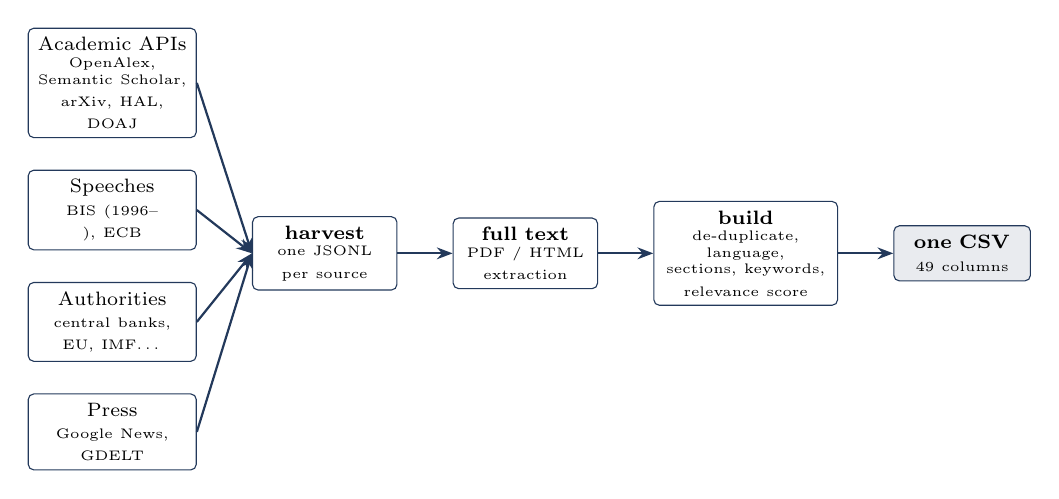
\begin{tikzpicture}[node distance=4mm and 7mm]
\node[box] (s1) {Academic APIs\\\tiny OpenAlex, Semantic Scholar,\\\tiny arXiv, HAL, DOAJ};
\node[box, below=of s1] (s2) {Speeches\\\tiny BIS (1996--), ECB};
\node[box, below=of s2] (s3) {Authorities\\\tiny central banks, EU, IMF\dots};
\node[box, below=of s3] (s4) {Press\\\tiny Google News, GDELT};
\node[box, right=of s2, yshift=-5.5mm, text width=16mm] (raw) {\textbf{harvest}\\\tiny one JSONL\\\tiny per source};
\node[box, right=of raw, text width=16mm] (ft) {\textbf{full text}\\\tiny PDF / HTML\\\tiny extraction};
\node[box, right=of ft, text width=21mm] (bd) {\textbf{build}\\\tiny de-duplicate, language,\\\tiny sections, keywords,\\\tiny relevance score};
\node[box, right=of bd, text width=15mm, fill=c1!10] (csv) {\textbf{one CSV}\\\tiny 49 columns};
\foreach \s in {s1,s2,s3,s4} \draw[arr] (\s.east) -- (raw.west);
\draw[arr] (raw) -- (ft); \draw[arr] (ft) -- (bd); \draw[arr] (bd) -- (csv);
\end{tikzpicture}
\end{center}
\small
\begin{itemize}
\item 115 search phrases, 12 languages: \emph{CBDC, digital euro, e-CNY, eNaira, Drex, digital fiat currency, Fedcoin, euro numérique, digitaler Euro, digital ruble\dots}
\item \alert{Recall first}: collect everything, then filter in four steps: homonyms, centrality, labels, \alert{economists}.
\end{itemize}
\note{\textbf{Slide 8} \hfill \textbf{Time: 0:40} \quad clock at the end of the slide: \textbf{5:20} / 25:55\\[3pt]
\textbf{Say:} Four families of sources: academic databases (OpenAlex, Semantic Scholar, arXiv, HAL, DOAJ), central bank speeches (BIS archive since 1996, ECB), central bank and institution websites, and the press.
115 search phrases in 12 languages: CBDC, digital euro, e-CNY, eNaira, euro num\'erique, digitaler Euro, digital ruble...
Principle: \textbf{recall first}. Collect everything, then filter in four steps. The fourth is the one the course asked for: is it written by an economist?}
\end{frame}

% STEP 1, HOMONYMS. Real code on the slide (fragile frame + listings) to show that the filter is
% explicit and reproducible. Term list in config.py.
% Rule: count(t) = n_t * 1[t not ambiguous OR monetary context]. Ambiguous terms (CBDC, DCEP, digital
% pound, digital yen...) count only if the title/keywords/abstract, or the body, contain monetary
% context (currency, payment, central bank, monnaie, Geld...). Records found by a CBDC-specific search
% get the context for free (press headlines are too short to carry it).
% "Digital dollar" and "Sand Dollar" are never scored: too ambiguous (stablecoins, a crypto, a
% beach...). They are reported, so we can see them, but they never make a text relevant.
\begin{frame}[fragile]{Step 1: is it really \emph{Central Bank Digital Currency}?}
\begin{columns}[T]
\begin{column}{0.5\textwidth}
\begin{lstlisting}
TERMS = {
  "CBDC": r"\bCBDCs?\b|\bwCBDCs?\b|\brCBDCs?\b",
  "central bank digital currency":
      r"central[\s-]+banks?(?:['’]s?)?[\s-]+"
      r"digital[\s-]+currenc(?:y|ies)",
  "digital euro": r"digital(?:e[rn]?)?\s+euro\b"
      r"|euro\s+numérique|euro\s+digitale?\b",
  "DCEP (e-CNY)": r"\bDC/?EP\b",
  ...
}
\end{lstlisting}
\end{column}
\begin{column}{0.47\textwidth}\small
\begin{itemize}
\item ``CBDC'' is also a \emph{skin disease}; ``DCEP'' a chemical.
\item Ambiguous terms $t\in\mathcal{A}$ count only with \alert{monetary context}:
\end{itemize}
\[
\text{count}(t) = n_t \cdot \mathbf{1}\big[t \notin \mathcal{A} \,\lor\, \text{context}\big]
\]
\begin{itemize}
\item context = \emph{currency, payment, central bank, monnaie, Geld\dots}
\item \emph{digital dollar}, \emph{Sand Dollar}: reported, never scored.
\end{itemize}
\end{column}
\end{columns}
\note{\textbf{Slide 9} \hfill \textbf{Time: 0:30} \quad clock at the end of the slide: \textbf{5:50} / 25:55\\[3pt]
\textbf{Say:} Step 1 removes homonyms. ``CBDC'' is also a skin disease in medical papers, ``DCEP'' a chemical. Ambiguous terms only count when the text also talks about money: currency, payment, central bank, in several languages.
``Digital dollar'' and ``Sand Dollar'' are recorded but never scored.}
\end{frame}

% STEP 2, THEME SCORE: THE WEIGHTS.
%   Each available field f gets a centrality c_f in [0,1]:
%     title    1 if a CBDC term is in the title (a title is the author's own statement of the topic)
%     keywords 0.4 if CBDC is in the keywords. Weight 0.4, not 1: keywords are partly machine-assigned
%              (OpenAlex, Semantic Scholar), so they are supporting evidence only. Alone, keywords give
%              100*(0.6*0.4 + 0.4*0.4) = 40: "secondary theme", never "main theme".
%     abstract share of its sentences that mention a CBDC (a whole abstract on CBDCs -> close to 1)
%     body     1/2 density + 1/2 spread. Density = mentions per 1,000 words, saturating at 3 (a text
%              devoted to CBDCs easily exceeds 3; saturation stops repetition from being rewarded).
%              Spread = share of the ten equal slices of the text that mention CBDCs: distinguishes a
%              text about CBDCs from start to end from one paragraph that names them ten times.
%              Only for bodies over 300 words.
%   score = 100 * (0.6 * max_f c_f + 0.4 * mean_f c_f), F = fields available.
%     0.6 on the max: one field clearly about CBDCs suffices (a paper with CBDC in its title is about
%     CBDCs even without an abstract). 0.4 on the mean: agreement across fields raises the score, so a
%     title mention contradicted by an abstract that never mentions it scores lower (80 instead of 100).
%     Mean over AVAILABLE fields: a record without abstract or full text is not penalised.
%   Worked examples (backup slide "how the relevance score behaves"): CBDC in title -> 87; one passing
%   mention in a long paper -> about 11 (body 0.1 -> 100*(0.06+0.04)).
%   Thresholds: >= 50 main theme, 25-49 secondary, < 25 mentioned only. 50 = a field clearly about
%   CBDCs; checked on the next slide by reading.
%   Why not a classifier? It would need thousands of labels and would be a black box; the score is
%   transparent, and its labels are validated by reading (next slide).
\begin{frame}{Step 2: how central is CBDC to the text?}
Each available field $f$ gets a centrality $c_f \in [0,1]$:
\begin{align*}
c_{\text{title}} &= \mathbf{1}[\text{CBDC term in title}] &
c_{\text{kw}} &= 0.4\cdot\mathbf{1}[\text{CBDC in keywords}]\\
c_{\text{abs}} &= \frac{\#\{\text{sentences mentioning CBDC}\}}{\#\{\text{sentences}\}} &
c_{\text{body}} &= \tfrac12\min\!\Big(1,\frac{\rho}{3}\Big) + \tfrac12\,\sigma
\end{align*}
$\rho$ = mentions per 1{,}000 words; $\sigma$ = share of the ten slices of the text that mention CBDC.
\[
\boxed{\text{score} = 100\Big(0.6\,\max_{f\in F} c_f + 0.4\,\frac{1}{|F|}\sum_{f\in F} c_f\Big)}
\qquad F = \text{fields available}
\]
\small One field clearly about CBDC suffices; a passing mention stays low; missing fields are not penalised.
\note{\textbf{Slide 10} \hfill \textbf{Time: 0:30} \quad clock at the end of the slide: \textbf{6:20} / 25:55\\[3pt]
\textbf{Say:} Step 2: how central is CBDC to the text, from 0 to 100.
Each field gets a centrality: the title (1 if it names a CBDC), the keywords (only 0.4, because databases assign them partly by machine), the abstract (share of its sentences on CBDCs), the body (how dense and how spread out the mentions are).
The score is 60\% the strongest field and 40\% the average: one field clearly about CBDCs is enough, a passing mention stays low, and missing fields do not count against a text.
\textbf{If asked "why 0.6/0.4?"}: chosen so that a title alone makes a main theme, keywords alone never do, and a passing mention scores about 10; then validated by reading (next slide).}
\end{frame}

% STEP 3, VALIDATION OF THE FILTER. 138 texts read blind to their label, stratified by label (about
% 20-30 per stratum), because a simple random sample would contain almost no "mentioned only" texts.
% Weights: precision and recall are recomputed with each stratum h weighted by its size N_h, so the
% oversampled small strata do not distort the totals:
%   P = sum_{h in T} N_h p_h / sum_{h in T} N_h ; R = sum_{h in T} N_h p_h / sum_h N_h p_h, T = kept labels.
% Wilson intervals because the strata are small and some shares are 0 or 1.
% Result: precision 0.89, recall 0.89. "Secondary theme" is noisy (11/29): hence the robustness check
% on main theme only. Pre-2014 records (32) were all checked false positives: hence 2014 as the start.
\begin{frame}{Step 3: labels, and how good is the filter?}
\begin{columns}[T]
\begin{column}{0.58\textwidth}\scriptsize
\setlength{\tabcolsep}{3pt}
\begin{tabular}{@{}lrrr@{}}\toprule
\textbf{Label (all texts kept)} & \textbf{Texts} & \textbf{Theme} & \textbf{95\% CI}\\\midrule
Main theme ($\geq 50$) & 15,464 & 29/30 & 0.83--0.99 \\
Secondary theme (25--49) & 2,245 & 11/29 & 0.23--0.56 \\
Mentioned only ($<25$) & 489 & 1/30 & 0.01--0.17 \\
Press, text not available & 13,446 & 2/19 & 0.03--0.31 \\
Ambiguous terms only & 1,709 & 3/10 & 0.11--0.60 \\
Off-topic (homonyms, no match) & 14,803 & 0/20 & 0.00--0.16 \\
Dated before 2014 (checked: false) & 32 & -- & -- \\
\bottomrule\end{tabular}\\[3pt]
Theme = share read as having CBDC as a theme, in a stratified sample of 138 texts read blind to the label; Wilson intervals.
\end{column}
\begin{column}{0.4\textwidth}\small
Strata $h$ weighted by size $N_h$; $T$ = theme labels:
\[ \widehat{P} = \frac{\sum_{h\in T} N_h \hat p_h}{\sum_{h\in T} N_h}, \qquad \widehat{R} = \frac{\sum_{h\in T} N_h \hat p_h}{\sum_{h} N_h \hat p_h} \]
\begin{itemize}\setlength\itemsep{1pt}
\item Precision \alert{0.89}, recall \alert{0.89}.
\item Secondary theme is noisy $\Rightarrow$ robustness on main theme only.
\end{itemize}
\end{column}
\end{columns}
\vspace{2pt}
\small Kept: \alert{main + secondary theme} (17,709 texts).
\note{\textbf{Slide 11} \hfill \textbf{Time: 0:40} \quad clock at the end of the slide: \textbf{7:00} / 25:55\\[3pt]
\textbf{Say:} Step 3: we read 138 texts without seeing their label. 29 of 30 ``main theme'' texts really are about CBDCs, none of the off-topic ones are.
Weighted by the size of each group, the filter has a precision and a recall of 0.89.
The ``secondary theme'' group is noisy (11 of 29), so every result is re-run on main-theme texts only (robustness slide).
We keep main and secondary theme: 17,709 texts.}
\end{frame}

% STEP 4, ECONOMISTS (the teacher's requirement). One table, kept and dropped side by side, so the
% audience sees what is excluded and how much.
%   Research kept if (1) OpenAlex primary topic field = "Economics, Econometrics and Finance" (OpenAlex
%   assigns it from title, abstract, venue and citations), or (2) an author is affiliated with a
%   central bank, the IMF or the BIS (regex on OpenAlex institutions), or (3) no OpenAlex record but an
%   economics venue (regex on the venue name). Order of the rules = order of the rows.
%   Speeches and central bank / international institution documents are kept as INSTITUTIONAL voices:
%   speeches are prepared with the bank's economics staff, even when the speaker is a lawyer.
%   Dropped: other fields (largest: computer science 1,769), governments and parliaments (politicians),
%   the press (no author, journalists).
% Why field and affiliation, not training? Authors' degrees are not recorded at scale; field and
% employer are what bibliometrics uses to define a discipline. Limit stated in the conclusion.
\begin{frame}{Step 4: is it written by an economist?}
\slabel{r:econ}
\footnotesize
\begin{tabular}{@{}p{0.62\textwidth}rl@{}}\toprule
\textbf{Texts with CBDC as a theme} & \textbf{Texts} & \\\midrule
Research, classified in economics or finance (OpenAlex) & 3,783 & kept \\
Research, other field but an author at a central bank, IMF or BIS & 148 & kept \\
Research without OpenAlex record, economics venue & 63 & kept \\
Research in other fields & 3,469 & dropped \\
Central bank speeches & 511 & kept \\
Documents of central banks and international institutions & 205 & kept \\
Documents of governments and parliaments & 34 & dropped \\
Press articles (no author) & 9,496 & dropped \\
\bottomrule\end{tabular}\\[4pt]
\scriptsize Field = OpenAlex primary topic (``Economics, Econometrics and Finance''); institutions = authors' affiliations in OpenAlex. Research dropped: Computer Science 1,769, Business, Management and Accounting 663, no OpenAlex record 473, Social Sciences 281.\\[4pt]
\small
\begin{itemize}\setlength\itemsep{1pt}
\item \alert{4,710 texts by economists}: research economists, and central banks and international institutions (staff economists, institutional voice).
\item Press dropped: no author is known, and journalists are not economists.
\end{itemize}
\method{m:econ}
\note{\textbf{Slide 12} \hfill \textbf{Time: 0:50} \quad clock at the end of the slide: \textbf{7:50} / 25:55\\[3pt]
\textbf{Say:} Step 4 answers the course's question: is the text written by an economist?
\begin{itemize}
\item Research is kept if OpenAlex classifies it in economics and finance, or if an author works at a central bank, the IMF or the BIS, or, without an OpenAlex record, if it appears in an economics outlet.
\item Central bank speeches and documents are kept as institutional voices.
\item Dropped: research in other fields (computer science first), governments and parliaments, the press.
\end{itemize}
Result: \textbf{4,710 texts by economists}: about 4,000 research texts, 511 speeches, 205 documents.
\textbf{If asked "a speech by a lawyer governor?"}: kept, as the institution's voice, written with its economists; the robustness slide also shows the results with every discipline.}
\end{frame}

% SOURCES AND COMPLETENESS. Two messages: where texts come from (a text found in two databases counts
% in both, hence a sum above 4,710), and which fields exist. The second table matters for the rest:
% each analysis runs on the texts that have its input (co-citation: reference lists, 32% only; tone:
% English CBDC sentences; motivations: introduction or abstract), so n changes from slide to slide.
\begin{frame}{Sources and completeness (economists' corpus)}
\begin{columns}[T]
\begin{column}{0.46\textwidth}\footnotesize
\begin{tabular}{@{}lr@{}}\toprule
\textbf{Database} & \textbf{Documents}\\\midrule
OpenAlex & 4,043 \\
Semantic Scholar & 2,164 \\
BIS central bankers' speeches & 465 \\
DOAJ & 251 \\
Central banks \& authorities (crawl) & 205 \\
ECB speeches & 108 \\
HAL & 31 \\
arXiv & 24 \\
\bottomrule\end{tabular}\\[2pt]
\scriptsize Merged duplicates count in each database.
\end{column}
\begin{column}{0.5\textwidth}\footnotesize
\begin{tabular}{@{}lr@{}}\toprule
\textbf{Type of text} & \textbf{Documents}\\\midrule
Academic & 3,994 \\
Speeches & 511 \\
Official docs & 205 \\
\midrule Total & 4,710\\\bottomrule\end{tabular}\\[6pt]
\begin{tabular}{@{}lr@{}}\toprule
\textbf{Field available} & \textbf{Share}\\\midrule
Exact day of publication & 71\% \\
Issuer / outlet identified & 97\% \\
Abstract & 68\% \\
Full text & 63\% \\
Keywords & 85\% \\
Reference list & 32\% \\
\bottomrule\end{tabular}
\end{column}
\end{columns}
\note{\textbf{Slide 13} \hfill \textbf{Time: 0:30} \quad clock at the end of the slide: \textbf{8:20} / 25:55\\[3pt]
\textbf{Say:} OpenAlex brings most research, the BIS archive most speeches. A text found in two databases is merged and counted in both.
Completeness: exact day for 71\%, abstract 68\%, full text 63\%, reference lists only 32\%. Each analysis uses the texts that have its input; the number of texts is always on the slide.
\textit{If short of time: one sentence.}}
\end{frame}

% GROWTH. Stacked bars by type, so the total height is the volume and the colours show the mix;
% research (navy, first in the stack) dominates and is kept at the bottom so its growth reads against
% the axis. Legend inside the plot (top left, empty space). 2026 is a partial year (to October): said
% in the footnote rather than shading the bar, to keep the chart clean.
% Growth rate = compound annual rate g = (N_2025/N_2017)^(1/8) - 1 = (839/20)^(1/8) - 1 = 60% (research).
% Turning point 2020: Libra (June 2019), COVID (cash and contactless), the ECB report (October 2020).
\begin{frame}{A literature that took off after 2020}
\slabel{r:growth}
\begin{columns}[c]
\begin{column}{0.66\textwidth}
\begin{tikzpicture}
\begin{axis}[ybar stacked, width=\textwidth, height=0.7\textheight, bar width=11pt,
  cycle list name=corpus, xtick=data, xticklabel style={/pgf/number format/1000 sep=, font=\scriptsize, rotate=45, anchor=north east},
  ymin=0, legend style={at={(0.02,0.98)},anchor=north west,font=\scriptsize,draw=none},
  ylabel={Documents}, tick label style={font=\scriptsize}, axis lines*=left, ymajorgrids]
\addplot coordinates {(2016,3) (2017,20) (2018,36) (2019,77) (2020,161) (2021,284) (2022,315) (2023,572) (2024,623) (2025,839) (2026,898)};
\addlegendentry{Academic}
\addplot coordinates {(2016,3) (2017,8) (2018,30) (2019,24) (2020,41) (2021,66) (2022,77) (2023,67) (2024,67) (2025,72) (2026,56)};
\addlegendentry{Speeches}
\addplot coordinates {(2016,1) (2017,5) (2018,2) (2019,2) (2020,9) (2021,7) (2022,12) (2023,49) (2024,30) (2025,45) (2026,42)};
\addlegendentry{Official docs}
\end{axis}
\end{tikzpicture}
\end{column}
\begin{column}{0.32\textwidth}\small
\begin{itemize}
\item From 103 in 2019 to 956 in 2025.
\item Growth 60\% a year.
\item Turning point 2020: Libra (2019), COVID, the ECB report (Oct.\ 2020).
\end{itemize}
\scriptsize 0 documents before 2016; 2026 runs to October.
\end{column}
\end{columns}
\note{\textbf{Slide 14} \hfill \textbf{Time: 0:30} \quad clock at the end of the slide: \textbf{8:50} / 25:55\\[3pt]
\textbf{Say:} Nothing before 2016; from about 100 texts in 2019 to 956 in 2025; research grows by 60\% a year. 2026 already exceeds 2025 by October.
The turning point is 2020: Libra in 2019, COVID, and the ECB's report on a digital euro in October 2020.}
\end{frame}

% LANGUAGES. Horizontal bars, sorted, values printed: languages are categories with long names, which
% read better on the y axis. English is left out of the chart (3,721 texts) or it would crush the
% others; its share is in the text. Message: Russian is a large second language (422), hence the
% multilingual tools and the Russia-related analysis later.
\begin{frame}{Languages}
\begin{columns}[c]
\begin{column}{0.58\textwidth}
\begin{tikzpicture}
\begin{axis}[xbar, width=\textwidth, height=0.72\textheight, bar width=7pt, xmin=0,
  symbolic y coords={{Arabic},{Turkish},{Japanese},{Italian},{Portuguese},{French},{Spanish},{Ukrainian},{German},{Russian}}, ytick=data, tick label style={font=\scriptsize},
  axis lines*=left, nodes near coords, nodes near coords style={font=\tiny},
  xlabel={Documents}, xlabel style={font=\scriptsize}, enlarge x limits={upper,value=0.12}]
\addplot[fill=c1, draw=c1] coordinates {(12,{Arabic}) (24,{Turkish}) (26,{Japanese}) (28,{Italian}) (31,{Portuguese}) (43,{French}) (74,{Spanish}) (91,{Ukrainian}) (94,{German}) (422,{Russian})};
\end{axis}
\end{tikzpicture}
\end{column}
\begin{column}{0.4\textwidth}\small
\begin{itemize}
\item English dominates: 3,721 texts (79\%); the chart shows the others.
\item Second language: \alert{Russian} (422 texts).
\item Everything kept in its original language: the topic model and the codebook are multilingual.
\end{itemize}
\end{column}
\end{columns}
\note{\textbf{Slide 15} \hfill \textbf{Time: 0:20} \quad clock at the end of the slide: \textbf{9:10} / 25:55\\[3pt]
\textbf{Say:} 79\% English, but Russian is a strong second (422 texts), mostly on the digital ruble. English-only databases would miss about a fifth of what economists write on CBDCs. Everything is kept in its language: the topic model and the codebook are multilingual.
\textit{If short of time: skip.}}
\end{frame}

% =====================================================================
\section{Who writes}

% WHO 1: RESEARCH ECONOMISTS. Left: outlets and laws; right: most cited papers (global citations from
% OpenAlex, not citations within our corpus: those are on the co-citation slide).
% Lotka: share of authors with n papers f(n) = C n^-beta, beta fitted by least squares on log-log
% counts; beta = 3.3 > 2 (mature fields): most authors write once (83%).
% Bradford: sources sorted by output, cut into three zones of 1/3 of the papers each: 21 : 310 : 1,148
% sources: a small core (21) and a very long tail (1,148 sources for the last third): a dispersed field.
% Message: working papers (SSRN, RePEc) weigh as much as journals; a young, open field.
\begin{frame}{Research economists: outlets, most cited, laws}
\slabel{r:research}
\begin{columns}[T]
\begin{column}{0.4\textwidth}\scriptsize\textbf{Main outlets}\\[2pt]
\begin{tabular}{@{}p{0.8\linewidth}r@{}}SSRN Electronic Journal & 461 \\
RePEc: Research Papers in Economics & 164 \\
Zenodo (CERN repository) & 126 \\
CyberLeninka (Russian repository) & 70 \\
Springer eBooks & 68 \\
Routledge eBooks & 56 \\
Ekonomika i Upravlenie & 47 \\\end{tabular}\\[4pt]
\textbf{Bibliometric laws.} Growth 60\%/year (2017--2025). Lotka: $f(n) \propto n^{-3.3}$, 83\% of authors publish once. Bradford: 21 core sources hold \nicefrac{1}{3} of the papers (zones 21 : 310 : 1,148).
\end{column}
\begin{column}{0.58\textwidth}\scriptsize\textbf{Most cited papers} (global citations)\\[2pt]
\begin{tabular}{@{}p{0.2\linewidth}p{0.66\linewidth}r@{}}
Bordo (2017) & Central Bank Digital Currency and the Future of Monetary\dots{} & 517 \\
Auer (2020) & Rise of the Central Bank Digital Currencies: Drivers, App\dots{} & 454 \\
Agur (2019) & Designing Central Bank Digital Currencies & 433 \\
Andolfatto (2020) & Assessing the Impact of Central Bank Digital Currency on\dots{} & 404 \\
Barrdear (2016) & The Macroeconomics of Central Bank Issued Digital Currenc\dots{} & 341 \\
\end{tabular}\\[6pt]
\small Working papers (SSRN, RePEc) weigh as much as journals; a young, open field: most authors write once.
\end{column}
\end{columns}
\method{m:laws}
\note{\textbf{Slide 16} \hfill \textbf{Time: 0:40} \quad clock at the end of the slide: \textbf{9:50} / 25:55\\[3pt]
\textbf{Say:} The biggest outlets are working-paper repositories, SSRN and RePEc, not journals: the debate happens before peer review.
The most cited papers are the classics from central bank and IMF economists: Bordo and Levin, Auer, Agur, Andolfatto, Barrdear and Kumhof.
Lotka: 83\% of authors write only once on CBDCs (exponent 3.3, against about 2 in mature fields). Bradford: 21 sources publish a third of the papers, the last third is spread over 1,148.
A young, open field, around a small core.}
\end{frame}

% WHO 2: VOICES. Three columns, same format, so that institutions are named as they are (the user
% asked to keep institutions "under the correct name"): speeches by central bank (BIS archive
% speaker's bank), documents by issuing institution, research by the authors' institutions (OpenAlex
% affiliations; a paper with authors at two institutions counts for both).
% Message: the ECB is the hub (digital euro); Russian universities are among the most active research
% institutions (digital ruble).
\begin{frame}{Who speaks: central banks, institutions, research centres}
\begin{columns}[T]\begin{column}{0.32\textwidth}\scriptsize\textbf{Speeches, by central bank}\\[2pt]\begin{tabular}{@{}p{0.8\linewidth}r@{}}European Central Bank & 118 \\
Deutsche Bundesbank & 63 \\
Bank of France & 49 \\
Hong Kong Monetary Authority & 23 \\
Federal Reserve Board & 21 \\
Bank of England & 21 \\
Bank of Italy & 19 \\
Bank of Japan & 14 \\\end{tabular}\end{column}\begin{column}{0.32\textwidth}\scriptsize\textbf{Documents, by institution}\\[2pt]\begin{tabular}{@{}p{0.8\linewidth}r@{}}European Central Bank & 98 \\
Bank of Japan & 27 \\
Sveriges Riksbank & 22 \\
Deutsche Bundesbank & 21 \\
Swiss National Bank & 9 \\
Central Bank of The Bahamas & 7 \\
Bank of Jamaica & 6 \\
Bank of Canada & 4 \\\end{tabular}\end{column}\begin{column}{0.32\textwidth}\scriptsize\textbf{Research, by author institution}\\[2pt]\begin{tabular}{@{}p{0.8\linewidth}r@{}}Financial University & 63 \\
European Central Bank & 61 \\
International Monetary Fund & 39 \\
Bank of Canada & 38 \\
The Russian Presidential Acad\dots{} & 33 \\
Bank for International Settle\dots{} & 32 \\
Moscow State Institute of Int\dots{} & 29 \\
Lomonosov Moscow State Univer\dots{} & 29 \\\end{tabular}\end{column}\end{columns}
\vspace{3pt}
\small \alert{European Central Bank} is the most vocal central bank: the digital euro makes it the hub of the debate.
\note{\textbf{Slide 17} \hfill \textbf{Time: 0:35} \quad clock at the end of the slide: \textbf{10:25} / 25:55\\[3pt]
\textbf{Say:} On the institutional side, the European Central Bank dominates: 118 speeches and 98 documents, because of the digital euro. Then the Bundesbank, the Banque de France, Hong Kong, the Fed, the Bank of England.
In research, the ECB, the IMF, the Bank of Canada and the BIS are among the top institutions, next to Russian universities (Financial University, Moscow State).}
\end{frame}

% CO-CITATION NETWORK. Two references are linked when the same paper cites both.
% Data: the 1,493 research texts with a reference list; references identified by normalised title (so
% that variants of the same work merge), 13,810 distinct references.
% Selection: the 40 most cited references; a link needs >= 2 co-citations (one co-citation is noise);
% references with fewer than 3 links are dropped (loosely attached, they blur the map); only the main
% connected component is drawn (one intellectual base).
% WEIGHT of a link: association strength s_ij = c_ij / (c_i c_j), proportional to observed / expected
% co-citations. Raw counts would link the most cited classics to everything; this weight removes
% popularity (van Eck & Waltman 2009, VOSviewer's default).
% Clusters: Louvain, maximising modularity Q with the same weights (seed fixed at 7, nodes sorted, so
% the result is identical at every run). Q = 0.10 is low: the clusters overlap, there are no schools.
% DRAWING: force-directed layout (Fruchterman-Reingold, 300 iterations, seed 3), pulled by the
% association strength, so co-cited works sit close; outliers pulled back to the edge of the cloud.
% Node radius = 0.6 + 2.6 sqrt(c_i / c_max) mm: AREA proportional to citations (the eye reads area,
% not radius). Edge opacity = 0.12 + 0.55 s_ij / s_max: strong links dark, weak links faint, so the
% structure shows without a hairball. Node colour = Louvain cluster.
% Right: the most cited works within the corpus (local citations), which differ from global ones.
\begin{frame}{Co-citation: the intellectual base}
\slabel{r:cocit}
\begin{columns}[T]
\begin{column}{0.7\textwidth}
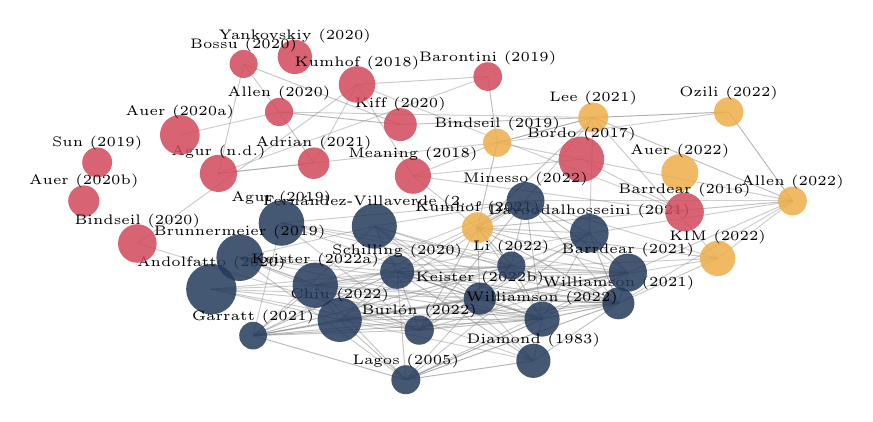
\begin{tikzpicture}
\draw[gray, opacity=0.67, line width=0.35pt] (6.47,3.33) -- (5.25,3.01);
\draw[gray, opacity=0.66, line width=0.35pt] (6.79,0.97) -- (5.03,1.03);
\draw[gray, opacity=0.66, line width=0.35pt] (4.09,0.00) -- (5.82,0.77);
\draw[gray, opacity=0.63, line width=0.35pt] (6.47,3.33) -- (8.19,3.40);
\draw[gray, opacity=0.63, line width=0.35pt] (6.79,0.97) -- (5.82,0.77);
\draw[gray, opacity=0.62, line width=0.35pt] (4.09,0.00) -- (6.79,0.97);
\draw[gray, opacity=0.60, line width=0.35pt] (5.82,0.77) -- (3.98,1.37);
\draw[gray, opacity=0.59, line width=0.35pt] (5.00,1.93) -- (5.43,1.45);
\draw[gray, opacity=0.58, line width=0.35pt] (5.43,1.45) -- (4.26,0.63);
\draw[gray, opacity=0.58, line width=0.35pt] (4.02,3.24) -- (2.48,3.40);
\draw[gray, opacity=0.58, line width=0.35pt] (4.09,0.00) -- (5.71,0.24);
\draw[gray, opacity=0.57, line width=0.35pt] (9.00,2.27) -- (8.19,3.40);
\draw[gray, opacity=0.56, line width=0.35pt] (6.79,0.97) -- (3.98,1.37);
\draw[gray, opacity=0.55, line width=0.35pt] (5.00,1.93) -- (6.79,0.97);
\draw[gray, opacity=0.55, line width=0.35pt] (5.03,1.03) -- (3.98,1.37);
\draw[gray, opacity=0.55, line width=0.35pt] (5.03,1.03) -- (5.82,0.77);
\draw[gray, opacity=0.55, line width=0.35pt] (4.09,0.00) -- (2.15,0.56);
\draw[gray, opacity=0.54, line width=0.35pt] (5.82,0.77) -- (5.43,1.45);
\draw[gray, opacity=0.54, line width=0.35pt] (6.79,0.97) -- (6.42,1.86);
\draw[gray, opacity=0.54, line width=0.35pt] (5.00,1.93) -- (5.03,1.03);
\draw[gray, opacity=0.54, line width=0.35pt] (5.82,0.77) -- (2.15,0.56);
\draw[gray, opacity=0.54, line width=0.35pt] (3.98,1.37) -- (2.15,0.56);
\draw[gray, opacity=0.52, line width=0.35pt] (5.61,2.27) -- (6.91,1.36);
\draw[gray, opacity=0.52, line width=0.35pt] (5.43,1.45) -- (2.15,0.56);
\draw[gray, opacity=0.52, line width=0.35pt] (5.25,3.01) -- (5.13,3.85);
\draw[gray, opacity=0.51, line width=0.35pt] (5.00,1.93) -- (5.25,3.01);
\draw[gray, opacity=0.51, line width=0.35pt] (6.42,1.86) -- (6.91,1.36);
\draw[gray, opacity=0.51, line width=0.35pt] (3.98,1.37) -- (5.71,0.24);
\draw[gray, opacity=0.51, line width=0.35pt] (5.82,0.77) -- (4.26,0.63);
\draw[gray, opacity=0.50, line width=0.35pt] (6.47,3.33) -- (4.02,3.24);
\draw[gray, opacity=0.50, line width=0.35pt] (6.79,0.97) -- (6.91,1.36);
\draw[gray, opacity=0.50, line width=0.35pt] (6.79,0.97) -- (5.43,1.45);
\draw[gray, opacity=0.50, line width=0.35pt] (6.47,3.33) -- (9.00,2.27);
\draw[gray, opacity=0.49, line width=0.35pt] (3.25,0.76) -- (2.15,0.56);
\draw[gray, opacity=0.49, line width=0.35pt] (5.82,0.77) -- (2.94,1.20);
\draw[gray, opacity=0.49, line width=0.35pt] (6.79,0.97) -- (2.15,0.56);
\draw[gray, opacity=0.49, line width=0.35pt] (5.00,1.93) -- (4.26,0.63);
\draw[gray, opacity=0.49, line width=0.35pt] (6.47,3.33) -- (5.00,1.93);
\draw[gray, opacity=0.49, line width=0.35pt] (5.61,2.27) -- (4.26,0.63);
\draw[gray, opacity=0.49, line width=0.35pt] (4.09,0.00) -- (3.25,0.76);
\draw[gray, opacity=0.49, line width=0.35pt] (9.00,2.27) -- (5.00,1.93);
\draw[gray, opacity=0.49, line width=0.35pt] (3.25,0.76) -- (5.82,0.77);
\draw[gray, opacity=0.48, line width=0.35pt] (3.98,1.37) -- (4.26,0.63);
\draw[gray, opacity=0.48, line width=0.35pt] (5.00,1.93) -- (8.05,1.54);
\draw[gray, opacity=0.48, line width=0.35pt] (6.79,0.97) -- (5.71,0.24);
\draw[gray, opacity=0.48, line width=0.35pt] (6.42,1.86) -- (5.61,2.27);
\draw[gray, opacity=0.47, line width=0.35pt] (4.09,0.00) -- (3.98,1.37);
\draw[gray, opacity=0.47, line width=0.35pt] (5.82,0.77) -- (6.91,1.36);
\draw[gray, opacity=0.47, line width=0.35pt] (5.03,1.03) -- (5.43,1.45);
\draw[gray, opacity=0.47, line width=0.35pt] (5.00,1.93) -- (5.61,2.27);
\draw[gray, opacity=0.47, line width=0.35pt] (3.69,1.95) -- (5.03,1.03);
\draw[gray, opacity=0.47, line width=0.35pt] (3.25,0.76) -- (3.98,1.37);
\draw[gray, opacity=0.47, line width=0.35pt] (5.61,2.27) -- (5.82,0.77);
\draw[gray, opacity=0.47, line width=0.35pt] (5.82,0.77) -- (5.71,0.24);
\draw[gray, opacity=0.46, line width=0.35pt] (3.69,1.95) -- (3.98,1.37);
\draw[gray, opacity=0.46, line width=0.35pt] (3.25,0.76) -- (2.94,1.20);
\draw[gray, opacity=0.46, line width=0.35pt] (5.61,2.27) -- (5.43,1.45);
\draw[gray, opacity=0.46, line width=0.35pt] (6.79,0.97) -- (3.69,1.95);
\draw[gray, opacity=0.46, line width=0.35pt] (2.15,0.56) -- (2.94,1.20);
\draw[gray, opacity=0.46, line width=0.35pt] (6.91,1.36) -- (4.26,0.63);
\draw[gray, opacity=0.46, line width=0.35pt] (3.25,0.76) -- (4.26,0.63);
\draw[gray, opacity=0.46, line width=0.35pt] (2.15,0.56) -- (6.91,1.36);
\draw[gray, opacity=0.46, line width=0.35pt] (4.02,3.24) -- (2.03,4.01);
\draw[gray, opacity=0.45, line width=0.35pt] (2.94,1.20) -- (4.26,0.63);
\draw[gray, opacity=0.45, line width=0.35pt] (5.61,2.27) -- (3.98,1.37);
\draw[gray, opacity=0.45, line width=0.35pt] (4.09,0.00) -- (2.94,1.20);
\draw[gray, opacity=0.45, line width=0.35pt] (2.48,3.40) -- (2.92,2.75);
\draw[gray, opacity=0.44, line width=0.35pt] (6.42,1.86) -- (5.82,0.77);
\draw[gray, opacity=0.44, line width=0.35pt] (4.09,0.00) -- (1.98,1.55);
\draw[gray, opacity=0.44, line width=0.35pt] (5.00,1.93) -- (6.91,1.36);
\draw[gray, opacity=0.44, line width=0.35pt] (2.15,0.56) -- (4.26,0.63);
\draw[gray, opacity=0.44, line width=0.35pt] (6.79,0.97) -- (5.61,2.27);
\draw[gray, opacity=0.43, line width=0.35pt] (5.03,1.03) -- (2.15,0.56);
\draw[gray, opacity=0.43, line width=0.35pt] (8.05,1.54) -- (6.79,0.97);
\draw[gray, opacity=0.43, line width=0.35pt] (1.62,1.15) -- (3.25,0.76);
\draw[gray, opacity=0.43, line width=0.35pt] (3.47,3.75) -- (5.13,3.85);
\draw[gray, opacity=0.43, line width=0.35pt] (5.00,1.93) -- (6.42,1.86);
\draw[gray, opacity=0.43, line width=0.35pt] (3.25,0.76) -- (5.43,1.45);
\draw[gray, opacity=0.43, line width=0.35pt] (5.03,1.03) -- (4.26,0.63);
\draw[gray, opacity=0.43, line width=0.35pt] (4.09,0.00) -- (6.91,1.36);
\draw[gray, opacity=0.43, line width=0.35pt] (3.25,0.76) -- (6.79,0.97);
\draw[gray, opacity=0.43, line width=0.35pt] (3.25,0.76) -- (5.03,1.03);
\draw[gray, opacity=0.43, line width=0.35pt] (3.98,1.37) -- (6.91,1.36);
\draw[gray, opacity=0.43, line width=0.35pt] (1.62,1.15) -- (5.82,0.77);
\draw[gray, opacity=0.43, line width=0.35pt] (5.03,1.03) -- (6.91,1.36);
\draw[gray, opacity=0.43, line width=0.35pt] (1.71,2.62) -- (2.03,4.01);
\draw[gray, opacity=0.43, line width=0.35pt] (3.98,1.37) -- (2.94,1.20);
\draw[gray, opacity=0.42, line width=0.35pt] (3.98,1.37) -- (1.98,1.55);
\draw[gray, opacity=0.42, line width=0.35pt] (5.43,1.45) -- (2.94,1.20);
\draw[gray, opacity=0.42, line width=0.35pt] (4.09,0.00) -- (6.42,1.86);
\draw[gray, opacity=0.42, line width=0.35pt] (3.47,3.75) -- (0.68,1.73);
\draw[gray, opacity=0.42, line width=0.35pt] (4.18,2.59) -- (3.47,3.75);
\draw[gray, opacity=0.42, line width=0.35pt] (4.09,0.00) -- (5.03,1.03);
\draw[gray, opacity=0.42, line width=0.35pt] (3.69,1.95) -- (2.15,0.56);
\draw[gray, opacity=0.42, line width=0.35pt] (6.79,0.97) -- (2.94,1.20);
\draw[gray, opacity=0.42, line width=0.35pt] (1.71,2.62) -- (2.92,2.75);
\draw[gray, opacity=0.42, line width=0.35pt] (5.82,0.77) -- (1.98,1.55);
\draw[gray, opacity=0.42, line width=0.35pt] (6.79,0.97) -- (4.26,0.63);
\draw[gray, opacity=0.42, line width=0.35pt] (6.42,1.86) -- (5.03,1.03);
\draw[gray, opacity=0.42, line width=0.35pt] (6.32,2.80) -- (7.63,2.13);
\draw[gray, opacity=0.42, line width=0.35pt] (1.62,1.15) -- (4.26,0.63);
\draw[gray, opacity=0.41, line width=0.35pt] (2.94,1.20) -- (6.91,1.36);
\draw[gray, opacity=0.41, line width=0.35pt] (4.18,2.59) -- (7.63,2.13);
\draw[gray, opacity=0.41, line width=0.35pt] (5.43,1.45) -- (6.91,1.36);
\draw[gray, opacity=0.41, line width=0.35pt] (5.61,2.27) -- (2.51,1.99);
\draw[gray, opacity=0.41, line width=0.35pt] (9.00,2.27) -- (6.42,1.86);
\draw[gray, opacity=0.41, line width=0.35pt] (9.00,2.27) -- (5.25,3.01);
\draw[gray, opacity=0.41, line width=0.35pt] (4.18,2.59) -- (5.25,3.01);
\draw[gray, opacity=0.41, line width=0.35pt] (6.47,3.33) -- (2.48,3.40);
\draw[gray, opacity=0.41, line width=0.35pt] (1.62,1.15) -- (3.98,1.37);
\draw[gray, opacity=0.41, line width=0.35pt] (6.47,3.33) -- (8.05,1.54);
\draw[gray, opacity=0.41, line width=0.35pt] (9.00,2.27) -- (6.91,1.36);
\draw[gray, opacity=0.41, line width=0.35pt] (1.98,1.55) -- (4.26,0.63);
\draw[gray, opacity=0.41, line width=0.35pt] (2.51,1.99) -- (6.91,1.36);
\draw[gray, opacity=0.41, line width=0.35pt] (6.47,3.33) -- (6.42,1.86);
\draw[gray, opacity=0.40, line width=0.35pt] (5.03,1.03) -- (2.94,1.20);
\draw[gray, opacity=0.40, line width=0.35pt] (3.25,0.76) -- (6.91,1.36);
\draw[gray, opacity=0.40, line width=0.35pt] (2.48,3.40) -- (2.03,4.01);
\draw[gray, opacity=0.40, line width=0.35pt] (4.18,2.59) -- (5.00,1.93);
\draw[gray, opacity=0.40, line width=0.35pt] (5.71,0.24) -- (1.98,1.55);
\draw[gray, opacity=0.40, line width=0.35pt] (4.26,0.63) -- (0.68,1.73);
\draw[gray, opacity=0.40, line width=0.35pt] (5.03,1.03) -- (5.71,0.24);
\draw[gray, opacity=0.40, line width=0.35pt] (6.79,0.97) -- (1.98,1.55);
\draw[gray, opacity=0.40, line width=0.35pt] (6.79,0.97) -- (2.51,1.99);
\draw[gray, opacity=0.40, line width=0.35pt] (5.00,1.93) -- (5.82,0.77);
\draw[gray, opacity=0.40, line width=0.35pt] (1.62,1.15) -- (2.94,1.20);
\draw[gray, opacity=0.40, line width=0.35pt] (3.69,1.95) -- (5.71,0.24);
\draw[gray, opacity=0.39, line width=0.35pt] (5.61,2.27) -- (2.94,1.20);
\draw[gray, opacity=0.39, line width=0.35pt] (3.69,1.95) -- (5.82,0.77);
\draw[gray, opacity=0.39, line width=0.35pt] (2.51,1.99) -- (4.26,0.63);
\draw[gray, opacity=0.39, line width=0.35pt] (8.05,1.54) -- (3.98,1.37);
\draw[gray, opacity=0.39, line width=0.35pt] (8.05,1.54) -- (5.61,2.27);
\draw[gray, opacity=0.39, line width=0.35pt] (5.25,3.01) -- (8.19,3.40);
\draw[gray, opacity=0.39, line width=0.35pt] (5.82,0.77) -- (2.51,1.99);
\draw[gray, opacity=0.39, line width=0.35pt] (3.69,1.95) -- (5.61,2.27);
\draw[gray, opacity=0.39, line width=0.35pt] (2.51,1.99) -- (2.15,0.56);
\draw[gray, opacity=0.39, line width=0.35pt] (9.00,2.27) -- (8.05,1.54);
\draw[gray, opacity=0.39, line width=0.35pt] (6.42,1.86) -- (5.43,1.45);
\draw[gray, opacity=0.39, line width=0.35pt] (3.47,3.75) -- (7.63,2.13);
\draw[gray, opacity=0.39, line width=0.35pt] (1.71,2.62) -- (5.13,3.85);
\draw[gray, opacity=0.39, line width=0.35pt] (3.69,1.95) -- (5.43,1.45);
\draw[gray, opacity=0.39, line width=0.35pt] (8.05,1.54) -- (5.03,1.03);
\draw[gray, opacity=0.39, line width=0.35pt] (1.71,2.62) -- (5.25,3.01);
\draw[gray, opacity=0.39, line width=0.35pt] (9.00,2.27) -- (6.79,0.97);
\draw[gray, opacity=0.39, line width=0.35pt] (3.25,0.76) -- (5.61,2.27);
\draw[gray, opacity=0.39, line width=0.35pt] (3.69,1.95) -- (1.98,1.55);
\draw[gray, opacity=0.39, line width=0.35pt] (1.98,1.55) -- (2.94,1.20);
\draw[gray, opacity=0.39, line width=0.35pt] (6.42,1.86) -- (4.26,0.63);
\draw[gray, opacity=0.39, line width=0.35pt] (2.48,3.40) -- (1.22,3.11);
\draw[gray, opacity=0.38, line width=0.35pt] (9.00,2.27) -- (5.61,2.27);
\draw[gray, opacity=0.38, line width=0.35pt] (1.62,1.15) -- (6.79,0.97);
\draw[gray, opacity=0.38, line width=0.35pt] (3.25,0.76) -- (5.71,0.24);
\draw[gray, opacity=0.38, line width=0.35pt] (5.61,2.27) -- (2.15,0.56);
\draw[gray, opacity=0.38, line width=0.35pt] (1.98,1.55) -- (6.91,1.36);
\draw[gray, opacity=0.38, line width=0.35pt] (6.42,1.86) -- (2.94,1.20);
\draw[gray, opacity=0.38, line width=0.35pt] (2.51,1.99) -- (5.43,1.45);
\draw[gray, opacity=0.38, line width=0.35pt] (3.47,3.75) -- (2.92,2.75);
\draw[gray, opacity=0.38, line width=0.35pt] (4.18,2.59) -- (6.32,2.80);
\draw[gray, opacity=0.38, line width=0.35pt] (3.98,1.37) -- (5.43,1.45);
\draw[gray, opacity=0.38, line width=0.35pt] (6.47,3.33) -- (5.61,2.27);
\fill[c2, opacity=0.85] (2.68,4.10) circle (2.18mm);
\node[font=\fontsize{4.6}{5}\selectfont, above=1.53mm, inner sep=0.5pt] at (2.68,4.10) {Yankovskiy (2020)};
\fill[c3, opacity=0.85] (6.47,3.33) circle (1.90mm);
\node[font=\fontsize{4.6}{5}\selectfont, above=1.33mm, inner sep=0.5pt] at (6.47,3.33) {Lee (2021)};
\fill[c3, opacity=0.85] (9.00,2.27) circle (1.83mm);
\node[font=\fontsize{4.6}{5}\selectfont, above=1.28mm, inner sep=0.5pt] at (9.00,2.27) {Allen (2022)};
\fill[c1, opacity=0.85] (1.62,1.15) circle (3.20mm);
\node[font=\fontsize{4.6}{5}\selectfont, above=2.24mm, inner sep=0.5pt] at (1.62,1.15) {Andolfatto (2020)};
\fill[c2, opacity=0.85] (4.02,3.24) circle (2.09mm);
\node[font=\fontsize{4.6}{5}\selectfont, above=1.46mm, inner sep=0.5pt] at (4.02,3.24) {Kiff (2020)};
\fill[c1, opacity=0.85] (4.09,0.00) circle (1.84mm);
\node[font=\fontsize{4.6}{5}\selectfont, above=1.29mm, inner sep=0.5pt] at (4.09,0.00) {Lagos (2005)};
\fill[c1, opacity=0.85] (3.25,0.76) circle (2.81mm);
\node[font=\fontsize{4.6}{5}\selectfont, above=1.97mm, inner sep=0.5pt] at (3.25,0.76) {Chiu (2022)};
\fill[c2, opacity=0.85] (4.18,2.59) circle (2.29mm);
\node[font=\fontsize{4.6}{5}\selectfont, above=1.61mm, inner sep=0.5pt] at (4.18,2.59) {Meaning (2018)};
\fill[c2, opacity=0.85] (1.71,2.62) circle (2.36mm);
\node[font=\fontsize{4.6}{5}\selectfont, above=1.65mm, inner sep=0.5pt] at (1.71,2.62) {Agur (n.d.)};
\fill[c2, opacity=0.85] (0.17,2.76) circle (1.90mm);
\node[font=\fontsize{4.6}{5}\selectfont, above=1.33mm, inner sep=0.5pt] at (0.17,2.76) {Sun (2019)};
\fill[c2, opacity=0.85] (3.47,3.75) circle (2.32mm);
\node[font=\fontsize{4.6}{5}\selectfont, above=1.63mm, inner sep=0.5pt] at (3.47,3.75) {Kumhof (2018)};
\fill[c3, opacity=0.85] (5.00,1.93) circle (1.97mm);
\node[font=\fontsize{4.6}{5}\selectfont, above=1.38mm, inner sep=0.5pt] at (5.00,1.93) {Kumhof (2021)};
\fill[c3, opacity=0.85] (7.57,2.63) circle (2.35mm);
\node[font=\fontsize{4.6}{5}\selectfont, above=1.64mm, inner sep=0.5pt] at (7.57,2.63) {Auer (2022)};
\fill[c3, opacity=0.85] (8.05,1.54) circle (2.24mm);
\node[font=\fontsize{4.6}{5}\selectfont, above=1.57mm, inner sep=0.5pt] at (8.05,1.54) {KIM (2022)};
\fill[c1, opacity=0.85] (6.79,0.97) circle (2.03mm);
\node[font=\fontsize{4.6}{5}\selectfont, above=1.42mm, inner sep=0.5pt] at (6.79,0.97) {Williamson (2021)};
\fill[c1, opacity=0.85] (6.42,1.86) circle (2.45mm);
\node[font=\fontsize{4.6}{5}\selectfont, above=1.72mm, inner sep=0.5pt] at (6.42,1.86) {Davoodalhosseini (2021)};
\fill[c2, opacity=0.85] (6.32,2.80) circle (2.89mm);
\node[font=\fontsize{4.6}{5}\selectfont, above=2.02mm, inner sep=0.5pt] at (6.32,2.80) {Bordo (2017)};
\fill[c1, opacity=0.85] (3.69,1.95) circle (2.86mm);
\node[font=\fontsize{4.6}{5}\selectfont, above=2.00mm, inner sep=0.5pt] at (3.69,1.95) {Fernández-Villaverde (2\dots{}};
\fill[c3, opacity=0.85] (5.25,3.01) circle (1.79mm);
\node[font=\fontsize{4.6}{5}\selectfont, above=1.25mm, inner sep=0.5pt] at (5.25,3.01) {Bindseil (2019)};
\fill[c1, opacity=0.85] (5.61,2.27) circle (2.41mm);
\node[font=\fontsize{4.6}{5}\selectfont, above=1.69mm, inner sep=0.5pt] at (5.61,2.27) {Minesso (2022)};
\fill[c3, opacity=0.85] (8.19,3.40) circle (1.87mm);
\node[font=\fontsize{4.6}{5}\selectfont, above=1.31mm, inner sep=0.5pt] at (8.19,3.40) {Ozili (2022)};
\fill[c1, opacity=0.85] (5.03,1.03) circle (2.05mm);
\node[font=\fontsize{4.6}{5}\selectfont, above=1.43mm, inner sep=0.5pt] at (5.03,1.03) {Keister (2022b)};
\fill[c1, opacity=0.85] (5.82,0.77) circle (2.23mm);
\node[font=\fontsize{4.6}{5}\selectfont, above=1.56mm, inner sep=0.5pt] at (5.82,0.77) {Williamson (2022)};
\fill[c1, opacity=0.85] (3.98,1.37) circle (2.16mm);
\node[font=\fontsize{4.6}{5}\selectfont, above=1.51mm, inner sep=0.5pt] at (3.98,1.37) {Schilling (2020)};
\fill[c2, opacity=0.85] (2.48,3.40) circle (1.79mm);
\node[font=\fontsize{4.6}{5}\selectfont, above=1.25mm, inner sep=0.5pt] at (2.48,3.40) {Allen (2020)};
\fill[c1, opacity=0.85] (2.51,1.99) circle (2.89mm);
\node[font=\fontsize{4.6}{5}\selectfont, above=2.02mm, inner sep=0.5pt] at (2.51,1.99) {Agur (2019)};
\fill[c1, opacity=0.85] (5.71,0.24) circle (2.17mm);
\node[font=\fontsize{4.6}{5}\selectfont, above=1.52mm, inner sep=0.5pt] at (5.71,0.24) {Diamond (1983)};
\fill[c2, opacity=0.85] (2.03,4.01) circle (1.78mm);
\node[font=\fontsize{4.6}{5}\selectfont, above=1.24mm, inner sep=0.5pt] at (2.03,4.01) {Bossu (2020)};
\fill[c1, opacity=0.85] (1.98,1.55) circle (2.96mm);
\node[font=\fontsize{4.6}{5}\selectfont, above=2.07mm, inner sep=0.5pt] at (1.98,1.55) {Brunnermeier (2019)};
\fill[c1, opacity=0.85] (5.43,1.45) circle (1.79mm);
\node[font=\fontsize{4.6}{5}\selectfont, above=1.25mm, inner sep=0.5pt] at (5.43,1.45) {Li (2022)};
\fill[c1, opacity=0.85] (2.15,0.56) circle (1.76mm);
\node[font=\fontsize{4.6}{5}\selectfont, above=1.24mm, inner sep=0.5pt] at (2.15,0.56) {Garratt (2021)};
\fill[c2, opacity=0.85] (5.13,3.85) circle (1.82mm);
\node[font=\fontsize{4.6}{5}\selectfont, above=1.27mm, inner sep=0.5pt] at (5.13,3.85) {Barontini (2019)};
\fill[c2, opacity=0.85] (1.22,3.11) circle (2.52mm);
\node[font=\fontsize{4.6}{5}\selectfont, above=1.76mm, inner sep=0.5pt] at (1.22,3.11) {Auer (2020a)};
\fill[c1, opacity=0.85] (2.94,1.20) circle (2.88mm);
\node[font=\fontsize{4.6}{5}\selectfont, above=2.02mm, inner sep=0.5pt] at (2.94,1.20) {Keister (2022a)};
\fill[c1, opacity=0.85] (6.91,1.36) circle (2.42mm);
\node[font=\fontsize{4.6}{5}\selectfont, above=1.70mm, inner sep=0.5pt] at (6.91,1.36) {Barrdear (2021)};
\fill[c2, opacity=0.85] (7.63,2.13) circle (2.45mm);
\node[font=\fontsize{4.6}{5}\selectfont, above=1.72mm, inner sep=0.5pt] at (7.63,2.13) {Barrdear (2016)};
\fill[c1, opacity=0.85] (4.26,0.63) circle (1.86mm);
\node[font=\fontsize{4.6}{5}\selectfont, above=1.30mm, inner sep=0.5pt] at (4.26,0.63) {Burlón (2022)};
\fill[c2, opacity=0.85] (2.92,2.75) circle (2.00mm);
\node[font=\fontsize{4.6}{5}\selectfont, above=1.40mm, inner sep=0.5pt] at (2.92,2.75) {Adrian (2021)};
\fill[c2, opacity=0.85] (0.00,2.27) circle (1.98mm);
\node[font=\fontsize{4.6}{5}\selectfont, above=1.38mm, inner sep=0.5pt] at (0.00,2.27) {Auer (2020b)};
\fill[c2, opacity=0.85] (0.68,1.73) circle (2.45mm);
\node[font=\fontsize{4.6}{5}\selectfont, above=1.71mm, inner sep=0.5pt] at (0.68,1.73) {Bindseil (2020)};
\end{tikzpicture}
\end{column}
\begin{column}{0.28\textwidth}\scriptsize
\textbf{Most cited within the corpus}\\[2pt]
\begin{tabular}{@{}lr@{}}Andolfatto (2020) & 264 \\
Brunnermeier (2019) & 218 \\
Bordo (2017) & 204 \\
Agur (2019) & 204 \\
Keister (2022) & 203 \\
Fernández-Villaverde (2020) & 199 \\
Chiu (2022) & 191 \\
Auer (2020) & 144 \\\end{tabular}
\end{column}
\end{columns}
\vspace{2pt}
\scriptsize\textbf{Clusters} (largest members):
\begin{itemize}\setlength\itemsep{0pt}
\item[\textcolor{c1}{$\bullet$}] Andolfatto (2020), Brunnermeier (2019), Agur (2019), Keister (2022a)
\item[\textcolor{c2}{$\bullet$}] Bordo (2017), Auer (2020a), Barrdear (2016), Bindseil (2020)
\item[\textcolor{c3}{$\bullet$}] Auer (2022), KIM (2022), Kumhof (2021), Lee (2021)
\end{itemize}
1,493 papers with reference lists, 13,810 distinct references; 40 most co-cited shown, 3 clusters, $Q=0.10$. \method{m:net}
\note{\textbf{Slide 18} \hfill \textbf{Time: 0:50} \quad clock at the end of the slide: \textbf{11:15} / 25:55\\[3pt]
\textbf{Say:} Two references are linked when the same paper cites them both; links are weighted so that popular classics are not linked to everything.
Three groups: Andolfatto, Brunnermeier, Agur, Keister (banking and design); Bordo, Auer, Barrdear, Bindseil (monetary policy and the first central bank studies); Auer 2022 and the recent Asian and design work.
But modularity is only 0.10: the groups overlap. \textbf{There are no separate schools}: everyone builds on the same core.
\textbf{If asked}: node area = citations; darker link = more often co-cited than expected.}
\end{frame}

% CO-AUTHORSHIP NETWORK. Authors linked when they sign a paper together.
% Identity: full name normalised (case, punctuation), NOT surname + initial, which would merge distinct
% people (every "Wang Y."). Papers with more than 25 authors (consortia) and institutional authors are
% excluded. The 80 most productive authors; a link from one joint paper; components of >= 3 authors.
% Weight and clusters: association strength + Louvain, as for co-citation.
% LAYOUT: the network is fragmented (teams), so each connected component is laid out in its own cell
% of a grid, largest first; otherwise small teams drift to the corners and the picture is unreadable.
% Same size / opacity encoding as co-citation.
% Right column: the numbers that the picture cannot show (share co-authored, team size, international
% share, countries) and the key fact of the section: central bank, BIS, IMF and World Bank authors
% write 10% of the papers but receive 48% of the citations (their share fell from 23% to 7%).
\begin{frame}{Co-authorship: research communities}
\slabel{r:coauth}
\begin{columns}[T]
\begin{column}{0.62\textwidth}
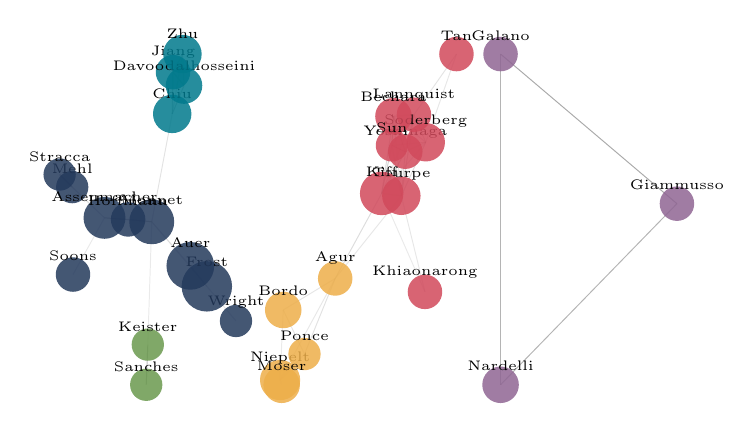
\begin{tikzpicture}
\draw[gray, opacity=0.67, line width=0.35pt] (5.60,4.20) -- (7.84,2.30);
\draw[gray, opacity=0.59, line width=0.35pt] (5.60,4.20) -- (5.60,0.00);
\draw[gray, opacity=0.59, line width=0.35pt] (5.60,0.00) -- (7.84,2.30);
\draw[gray, opacity=0.56, line width=0.35pt] (4.39,2.96) -- (4.22,3.04);
\draw[gray, opacity=0.52, line width=0.35pt] (0.16,2.51) -- (0.00,2.67);
\draw[gray, opacity=0.52, line width=0.35pt] (1.10,0.00) -- (1.12,0.51);
\draw[gray, opacity=0.51, line width=0.35pt] (4.39,2.96) -- (4.24,3.41);
\draw[gray, opacity=0.50, line width=0.35pt] (4.24,3.41) -- (4.22,3.04);
\draw[gray, opacity=0.43, line width=0.35pt] (1.44,3.97) -- (1.58,3.80);
\draw[gray, opacity=0.41, line width=0.35pt] (1.43,3.44) -- (1.58,3.80);
\draw[gray, opacity=0.40, line width=0.35pt] (1.44,3.97) -- (1.43,3.44);
\draw[gray, opacity=0.40, line width=0.35pt] (1.44,3.97) -- (1.56,4.20);
\draw[gray, opacity=0.36, line width=0.35pt] (4.09,2.43) -- (4.22,3.04);
\draw[gray, opacity=0.36, line width=0.35pt] (4.50,3.43) -- (4.24,3.41);
\draw[gray, opacity=0.34, line width=0.35pt] (4.50,3.43) -- (4.22,3.04);
\draw[gray, opacity=0.33, line width=0.35pt] (4.50,3.43) -- (4.34,2.40);
\draw[gray, opacity=0.32, line width=0.35pt] (4.39,2.96) -- (4.09,2.43);
\draw[gray, opacity=0.30, line width=0.35pt] (4.39,2.96) -- (4.50,3.43);
\draw[gray, opacity=0.30, line width=0.35pt] (1.17,2.07) -- (0.87,2.10);
\draw[gray, opacity=0.30, line width=0.35pt] (1.58,3.80) -- (1.56,4.20);
\draw[gray, opacity=0.29, line width=0.35pt] (4.09,2.43) -- (4.24,3.41);
\draw[gray, opacity=0.29, line width=0.35pt] (4.65,3.08) -- (4.22,3.04);
\draw[gray, opacity=0.29, line width=0.35pt] (4.34,2.40) -- (4.22,3.04);
\draw[gray, opacity=0.29, line width=0.35pt] (0.57,2.12) -- (0.87,2.10);
\draw[gray, opacity=0.27, line width=0.35pt] (4.65,3.08) -- (4.34,2.40);
\draw[gray, opacity=0.27, line width=0.35pt] (1.43,3.44) -- (1.56,4.20);
\draw[gray, opacity=0.27, line width=0.35pt] (4.34,2.40) -- (4.09,2.43);
\draw[gray, opacity=0.27, line width=0.35pt] (3.50,1.35) -- (4.09,2.43);
\draw[gray, opacity=0.26, line width=0.35pt] (4.39,2.96) -- (4.65,3.08);
\draw[gray, opacity=0.26, line width=0.35pt] (4.39,2.96) -- (4.34,2.40);
\draw[gray, opacity=0.26, line width=0.35pt] (4.50,3.43) -- (4.65,3.08);
\draw[gray, opacity=0.25, line width=0.35pt] (1.87,1.25) -- (1.66,1.51);
\draw[gray, opacity=0.25, line width=0.35pt] (0.16,2.51) -- (0.57,2.12);
\draw[gray, opacity=0.24, line width=0.35pt] (4.65,3.08) -- (4.24,3.41);
\draw[gray, opacity=0.24, line width=0.35pt] (4.34,2.40) -- (4.24,3.41);
\draw[gray, opacity=0.23, line width=0.35pt] (3.50,1.35) -- (3.11,0.39);
\draw[gray, opacity=0.22, line width=0.35pt] (1.17,2.07) -- (1.43,3.44);
\draw[gray, opacity=0.22, line width=0.35pt] (4.50,3.43) -- (4.09,2.43);
\draw[gray, opacity=0.21, line width=0.35pt] (3.11,0.39) -- (2.84,0.95);
\draw[gray, opacity=0.21, line width=0.35pt] (4.50,3.43) -- (5.04,4.20);
\draw[gray, opacity=0.20, line width=0.35pt] (2.24,0.81) -- (1.87,1.25);
\draw[gray, opacity=0.20, line width=0.35pt] (1.17,2.07) -- (0.57,2.12);
\draw[gray, opacity=0.20, line width=0.35pt] (3.50,1.35) -- (2.84,0.95);
\draw[gray, opacity=0.20, line width=0.35pt] (4.65,3.08) -- (4.09,2.43);
\draw[gray, opacity=0.19, line width=0.35pt] (2.80,0.06) -- (3.11,0.39);
\draw[gray, opacity=0.19, line width=0.35pt] (5.04,4.20) -- (4.65,3.08);
\draw[gray, opacity=0.19, line width=0.35pt] (4.34,2.40) -- (3.50,1.35);
\draw[gray, opacity=0.19, line width=0.35pt] (4.34,2.40) -- (4.64,1.18);
\draw[gray, opacity=0.18, line width=0.35pt] (2.80,0.06) -- (3.50,1.35);
\draw[gray, opacity=0.17, line width=0.35pt] (1.17,2.07) -- (1.12,0.51);
\draw[gray, opacity=0.17, line width=0.35pt] (0.57,2.12) -- (0.17,1.40);
\draw[gray, opacity=0.17, line width=0.35pt] (2.80,0.06) -- (2.84,0.95);
\draw[gray, opacity=0.17, line width=0.35pt] (2.80,0.06) -- (2.82,0.00);
\draw[gray, opacity=0.17, line width=0.35pt] (4.09,2.43) -- (4.64,1.18);
\draw[gray, opacity=0.16, line width=0.35pt] (1.17,2.07) -- (1.66,1.51);
\draw[gray, opacity=0.15, line width=0.35pt] (1.17,2.07) -- (1.87,1.25);
\fill[c2, opacity=0.85] (4.39,2.96) circle (2.19mm);
\node[font=\fontsize{4.6}{5}\selectfont, above=1.53mm, inner sep=0.5pt] at (4.39,2.96) {Yoshinaga};
\fill[c1, opacity=0.85] (2.24,0.81) circle (2.05mm);
\node[font=\fontsize{4.6}{5}\selectfont, above=1.44mm, inner sep=0.5pt] at (2.24,0.81) {Wright};
\fill[c1, opacity=0.85] (0.16,2.51) circle (2.05mm);
\node[font=\fontsize{4.6}{5}\selectfont, above=1.44mm, inner sep=0.5pt] at (0.16,2.51) {Mehl};
\fill[c2, opacity=0.85] (4.50,3.43) circle (2.19mm);
\node[font=\fontsize{4.6}{5}\selectfont, above=1.53mm, inner sep=0.5pt] at (4.50,3.43) {Lannquist};
\fill[c2, opacity=0.85] (5.04,4.20) circle (2.19mm);
\node[font=\fontsize{4.6}{5}\selectfont, above=1.53mm, inner sep=0.5pt] at (5.04,4.20) {Tan};
\fill[c1, opacity=0.85] (1.17,2.07) circle (2.85mm);
\node[font=\fontsize{4.6}{5}\selectfont, above=2.00mm, inner sep=0.5pt] at (1.17,2.07) {Monnet};
\fill[c6, opacity=0.85] (1.10,0.00) circle (2.05mm);
\node[font=\fontsize{4.6}{5}\selectfont, above=1.44mm, inner sep=0.5pt] at (1.10,0.00) {Sanches};
\fill[c3, opacity=0.85] (2.80,0.06) circle (2.55mm);
\node[font=\fontsize{4.6}{5}\selectfont, above=1.79mm, inner sep=0.5pt] at (2.80,0.06) {Niepelt};
\fill[c2, opacity=0.85] (4.65,3.08) circle (2.44mm);
\node[font=\fontsize{4.6}{5}\selectfont, above=1.71mm, inner sep=0.5pt] at (4.65,3.08) {Soderberg};
\fill[c5, opacity=0.85] (5.60,4.20) circle (2.19mm);
\node[font=\fontsize{4.6}{5}\selectfont, above=1.53mm, inner sep=0.5pt] at (5.60,4.20) {Galano};
\fill[c2, opacity=0.85] (4.34,2.40) circle (2.44mm);
\node[font=\fontsize{4.6}{5}\selectfont, above=1.71mm, inner sep=0.5pt] at (4.34,2.40) {Tourpe};
\fill[c3, opacity=0.85] (3.50,1.35) circle (2.19mm);
\node[font=\fontsize{4.6}{5}\selectfont, above=1.53mm, inner sep=0.5pt] at (3.50,1.35) {Agur};
\fill[c4, opacity=0.85] (1.44,3.97) circle (2.19mm);
\node[font=\fontsize{4.6}{5}\selectfont, above=1.53mm, inner sep=0.5pt] at (1.44,3.97) {Jiang};
\fill[c2, opacity=0.85] (4.09,2.43) circle (2.76mm);
\node[font=\fontsize{4.6}{5}\selectfont, above=1.93mm, inner sep=0.5pt] at (4.09,2.43) {Kiff};
\fill[c1, opacity=0.85] (1.87,1.25) circle (3.20mm);
\node[font=\fontsize{4.6}{5}\selectfont, above=2.24mm, inner sep=0.5pt] at (1.87,1.25) {Frost};
\fill[c4, opacity=0.85] (1.43,3.44) circle (2.44mm);
\node[font=\fontsize{4.6}{5}\selectfont, above=1.71mm, inner sep=0.5pt] at (1.43,3.44) {Chiu};
\fill[c3, opacity=0.85] (3.11,0.39) circle (2.05mm);
\node[font=\fontsize{4.6}{5}\selectfont, above=1.44mm, inner sep=0.5pt] at (3.11,0.39) {Ponce};
\fill[c1, opacity=0.85] (0.57,2.12) circle (2.66mm);
\node[font=\fontsize{4.6}{5}\selectfont, above=1.86mm, inner sep=0.5pt] at (0.57,2.12) {Assenmacher};
\fill[c1, opacity=0.85] (0.00,2.67) circle (2.05mm);
\node[font=\fontsize{4.6}{5}\selectfont, above=1.44mm, inner sep=0.5pt] at (0.00,2.67) {Stracca};
\fill[c2, opacity=0.85] (4.24,3.41) circle (2.32mm);
\node[font=\fontsize{4.6}{5}\selectfont, above=1.62mm, inner sep=0.5pt] at (4.24,3.41) {Bechara};
\fill[c5, opacity=0.85] (5.60,0.00) circle (2.32mm);
\node[font=\fontsize{4.6}{5}\selectfont, above=1.62mm, inner sep=0.5pt] at (5.60,0.00) {Nardelli};
\fill[c3, opacity=0.85] (2.84,0.95) circle (2.32mm);
\node[font=\fontsize{4.6}{5}\selectfont, above=1.62mm, inner sep=0.5pt] at (2.84,0.95) {Bordo};
\fill[c1, opacity=0.85] (0.17,1.40) circle (2.19mm);
\node[font=\fontsize{4.6}{5}\selectfont, above=1.53mm, inner sep=0.5pt] at (0.17,1.40) {Soons};
\fill[c1, opacity=0.85] (0.87,2.10) circle (2.19mm);
\node[font=\fontsize{4.6}{5}\selectfont, above=1.53mm, inner sep=0.5pt] at (0.87,2.10) {Hoffmann};
\fill[c1, opacity=0.85] (1.66,1.51) circle (3.03mm);
\node[font=\fontsize{4.6}{5}\selectfont, above=2.12mm, inner sep=0.5pt] at (1.66,1.51) {Auer};
\fill[c5, opacity=0.85] (7.84,2.30) circle (2.19mm);
\node[font=\fontsize{4.6}{5}\selectfont, above=1.53mm, inner sep=0.5pt] at (7.84,2.30) {Giammusso};
\fill[c4, opacity=0.85] (1.58,3.80) circle (2.32mm);
\node[font=\fontsize{4.6}{5}\selectfont, above=1.62mm, inner sep=0.5pt] at (1.58,3.80) {Davoodalhosseini};
\fill[c2, opacity=0.85] (4.64,1.18) circle (2.19mm);
\node[font=\fontsize{4.6}{5}\selectfont, above=1.53mm, inner sep=0.5pt] at (4.64,1.18) {Khiaonarong};
\fill[c2, opacity=0.85] (4.22,3.04) circle (2.05mm);
\node[font=\fontsize{4.6}{5}\selectfont, above=1.44mm, inner sep=0.5pt] at (4.22,3.04) {Sun};
\fill[c3, opacity=0.85] (2.82,0.00) circle (2.32mm);
\node[font=\fontsize{4.6}{5}\selectfont, above=1.62mm, inner sep=0.5pt] at (2.82,0.00) {Moser};
\fill[c6, opacity=0.85] (1.12,0.51) circle (2.05mm);
\node[font=\fontsize{4.6}{5}\selectfont, above=1.44mm, inner sep=0.5pt] at (1.12,0.51) {Keister};
\fill[c4, opacity=0.85] (1.56,4.20) circle (2.44mm);
\node[font=\fontsize{4.6}{5}\selectfont, above=1.71mm, inner sep=0.5pt] at (1.56,4.20) {Zhu};
\end{tikzpicture}
\end{column}
\begin{column}{0.36\textwidth}\scriptsize
\textbf{Most productive authors}\\[2pt]
\begin{tabular}{@{}lr@{}}Ulrich Bindseil & 20 \\
Peterson K Ozili & 20 \\
Jon Frost & 16 \\
Annelieke Mooij & 16 \\
Raphael Auer & 14 \\
Cyril Monnet & 12 \\
John Kiff & 11 \\
Katrin Assenmacher & 10 \\\end{tabular}\\[6pt]
5,716 authors; 48\% of papers co-authored (mean team 1.9); 15\% international. Top countries: RU 473, US 248, DE 167, CN 166, GB 153.\\[4pt]
Papers with a central bank, BIS, IMF or World Bank author: \alert{10\%} (23\% in 2014--2019, 7\% in 2023--2026), but \alert{48\% of citations}.
\end{column}
\end{columns}
\method{m:net}
\note{\textbf{Slide 19} \hfill \textbf{Time: 0:45} \quad clock at the end of the slide: \textbf{12:00} / 25:55\\[3pt]
\textbf{Say:} Teams are small: half the papers have one author, a team averages 1.9 people, 15\% are international. Each island on the map is a team: Bindseil's at the ECB, Auer and Frost at the BIS, Ozili alone but very productive.
Key fact: papers with a central bank, BIS, IMF or World Bank author are 10\% of papers but get \textbf{48\% of citations}. Their share fell from 23\% to 7\%: new papers come from outside these institutions, but the field still cites the institutions.}
\end{frame}

% LOG-ODDS. Words over-used by each group compared with the other.
% Weights: log-odds ratio with an informative Dirichlet prior (Monroe, Colaresi & Quinn 2008):
%   alpha_w = alpha_0 * (corpus frequency of w), alpha_0 = 500: each word gets 500 pseudo-occurrences
%   spread in proportion to its overall frequency. This shrinks rare words towards zero (a word used
%   twice by one group and never by the other does not come first) and the z-score divides by the
%   uncertainty. Vocabulary: words used at least 20 times; topic words (CBDC, digital, currency...)
%   and stop words removed, otherwise they would dominate both lists.
% Inputs: English only (the method compares word counts, so one language); research = title +
% abstract; central bankers = speeches (first 6,000 characters). Word totals shown under each header,
% so the audience sees the two corpora are of similar size (259k vs 232k words).
% Two columns, same length, z-scores right-aligned: a mirror, to read across.
\begin{frame}{Who says what: research economists vs central bankers}
\slabel{r:logodds}
\footnotesize
Words most over-used by each group compared with the other ($z$-scores):\\[4pt]
\begin{tabular}{@{}p{0.42\textwidth}p{0.42\textwidth}@{}}\toprule
\textbf{Research economists} \scriptsize(259,105 words) & \textbf{Central bankers} \scriptsize(232,446 words)\\\midrule
legal \hfill 23 & payments \hfill 28 \\
analysis \hfill 21 & euro \hfill 22 \\
development \hfill 21 & european \hfill 18 \\
research \hfill 20 & europe \hfill 18 \\
monetary \hfill 20 & area \hfill 18 \\
impact \hfill 19 & services \hfill 15 \\
model \hfill 18 & innovation \hfill 14 \\
implementation \hfill 17 & conference \hfill 14 \\
\bottomrule\end{tabular}\\[4pt]
\scriptsize English texts; research: title + abstract; central bankers: speeches; topic words (\emph{CBDC, digital, currency\dots}) removed.\\[3pt]
\small \alert{Reading}: research economists: \emph{legal, analysis, development}; central bankers: \emph{payments, euro, european}.
\method{m:logodds}
\note{\textbf{Slide 20} \hfill \textbf{Time: 0:40} \quad clock at the end of the slide: \textbf{12:40} / 25:55\\[3pt]
\textbf{Say:} Which words does each group use more than the other, once chance is accounted for?
Research economists: legal, analysis, development, model, impact: they \emph{analyse} CBDCs. Central bankers: payments, euro, Europe, services, innovation: they talk about \emph{their} project, the digital euro, as a payment instrument.
\textbf{If asked}: the method shrinks rare words, so a word used twice by one group cannot top the list.}
\end{frame}

% =====================================================================
\section{What is written}

% THEMATIC MAP (Callon; Cobo et al. 2011; as in bibliometrix).
% Keywords: author + indexed keywords, cleaned (plurals, generic and discipline words removed, a known
% mis-tag dropped); the 80 most frequent; a link needs >= 2 papers; clusters by Louvain on association
% strength.
% Axes: centrality(C) = 10 * sum_{i in C, j not in C} e_ij (links to other themes);
%       density(C) = 100/|C| * sum_{i,j in C} e_ij (internal cohesion), with the equivalence index
%       e_ij = c_ij^2 / (c_i c_j). The factors 10 and 100 are Callon's conventions, they only rescale.
% Quadrants split at the MEDIANS of the clusters (not at fixed values): positions are relative, which
% is all the map can say. Bubble radius = 2 + 4.5 sqrt(size / max) mm: area ~ number of keywords.
% Each cluster is named by its most frequent keywords; numbered so the table on the right can be read
% with the picture.
\begin{frame}{Thematic map: which themes drive the field?}
\slabel{r:thematic}
\begin{columns}[c]
\begin{column}{0.47\textwidth}
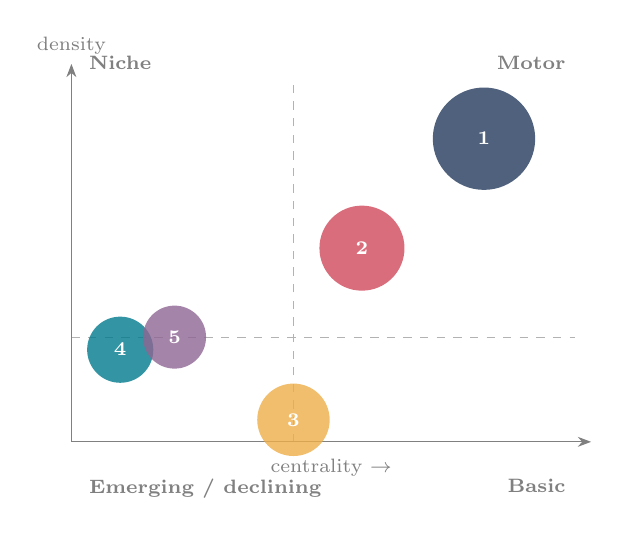
\begin{tikzpicture}[font=\scriptsize]
\draw[gray!60, dashed] (2.82,0) -- (2.82,4.6);
\draw[gray!60, dashed] (0,1.33) -- (6.4,1.33);
\draw[-{Stealth}, gray] (0,0) -- (6.6000000000000005,0) node[below, text=gray, pos=0.5, yshift=-1mm] {centrality $\to$};
\draw[-{Stealth}, gray] (0,0) -- (0,4.8) node[above, text=gray] {density};
\node[gray, anchor=south east, font=\scriptsize\bfseries] at (6.4,4.6) {Motor};
\node[gray, anchor=south west, font=\scriptsize\bfseries] at (0.1,4.6) {Niche};
\node[gray, anchor=north west, font=\scriptsize\bfseries] at (0.1,-0.35) {Emerging / declining};
\node[gray, anchor=north east, font=\scriptsize\bfseries] at (6.4,-0.35) {Basic};
\fill[c1, opacity=0.8] (5.24,3.85) circle (6.5mm);
\node[font=\scriptsize, text=white] at (5.24,3.85) {\textbf{1}};
\fill[c2, opacity=0.8] (3.69,2.46) circle (5.4mm);
\node[font=\scriptsize, text=white] at (3.69,2.46) {\textbf{2}};
\fill[c3, opacity=0.8] (2.82,0.28) circle (4.6mm);
\node[font=\scriptsize, text=white] at (2.82,0.28) {\textbf{3}};
\fill[c4, opacity=0.8] (0.62,1.17) circle (4.2mm);
\node[font=\scriptsize, text=white] at (0.62,1.17) {\textbf{4}};
\fill[c5, opacity=0.8] (1.31,1.33) circle (4.0mm);
\node[font=\scriptsize, text=white] at (1.31,1.33) {\textbf{5}};
\end{tikzpicture}
\end{column}
\begin{column}{0.51\textwidth}\scriptsize
Keyword clusters placed by \alert{centrality} (links to other themes) and \alert{density} (internal cohesion).\\[3pt]
\begin{tabular}{@{}lp{0.62\linewidth}l@{}}\toprule
 & \textbf{Theme} (top keywords) & \textbf{Quadrant}\\\midrule
\textcolor{c1}{\textbf{1}} & digital transformation in financial services, monetary policy, moneta\dots{} & motor \\
\textcolor{c2}{\textbf{2}} & blockchain technology applications and security, digital transformati\dots{} & motor \\
\textcolor{c3}{\textbf{3}} & fintech, crowdfunding, digital finance, blockchain, fintech & basic \\
\textcolor{c4}{\textbf{4}} & global financial crisis and policies, international payments, stablec\dots{} & emerging or declining \\
\textcolor{c5}{\textbf{5}} & financial inclusion, digital payments, india & niche \\
\bottomrule\end{tabular}\\[3pt]
\small Motor themes: digital transformation in financial services; blockchain technology applications and security.
\end{column}
\end{columns}
\method{m:callon}
\note{\textbf{Slide 21} \hfill \textbf{Time: 0:45} \quad clock at the end of the slide: \textbf{13:25} / 25:55\\[3pt]
\textbf{Say:} Each bubble is a group of keywords that appear together. Horizontal: how linked the theme is to the rest of the field; vertical: how developed it is inside.
Motor themes (top right): digital transformation of finance with monetary policy, and blockchain technology. Fintech is a basic theme. Financial inclusion with India and digital payments is a niche. Global financial crisis and stablecoins sits in emerging or declining.
\textbf{If asked}: quadrants are split at the medians, so positions are relative.}
\end{frame}

% EVOLUTION OF KEYWORDS. Share of each period's research papers carrying the keyword (not raw counts,
% which would all rise with the field). The 16 most frequent keywords; three periods chosen before
% looking at the data: 2014-19 (before the ECB report), 2020-22 (reports and pilots), 2023-26
% (legislation and launches). Sorted by the change between the last two periods; heat shading;
% teal = up, red = down. The number of papers per period is printed (136 / 755 / 2,919) because the
% first period is small. Last line: c-TF-IDF with each period as a class (what is NEW in each period).
\begin{frame}{How the themes evolve}
\slabel{r:evo}
\scriptsize
\begin{tabular}{@{}p{0.42\textwidth}rrrr@{}}\toprule
\textbf{Keyword} (\% of the period's papers) & \textbf{2014--2019} & \textbf{2020--2022} & \textbf{2023--2026} & \textbf{Change}\\
\textit{papers in period} & \textit{136} & \textit{755} & \textit{2,919} &\\\midrule
financial inclusion & \cellcolor{c1!5}5.9 & \cellcolor{c1!8}8.2 & \cellcolor{c1!15}15.8 & \textcolor{c4}{$+7.6$} \\
digital euro & \cellcolor{c1!2}2.9 & \cellcolor{c1!7}7.8 & \cellcolor{c1!11}11.4 & \textcolor{c4}{$+3.6$} \\
global financial crisis and policies & \cellcolor{c1!2}2.2 & \cellcolor{c1!8}8.7 & \cellcolor{c1!11}11.8 & \textcolor{c4}{$+3.0$} \\
financial stability & \cellcolor{c1!24}24.3 & \cellcolor{c1!12}12.6 & \cellcolor{c1!15}15.6 & \textcolor{c4}{$+3.0$} \\
fintech, crowdfunding, digital finance & \cellcolor{c1!48}48.5 & \cellcolor{c1!48}48.7 & \cellcolor{c1!49}49.8 & \textcolor{c4}{$+1.0$} \\
digital ruble & \cellcolor{c1!0}0.0 & \cellcolor{c1!13}13.9 & \cellcolor{c1!14}14.8 & \textcolor{c4}{$+0.9$} \\
european monetary and fiscal policies & \cellcolor{c1!16}16.9 & \cellcolor{c1!10}10.3 & \cellcolor{c1!10}10.3 & \textcolor{c2}{$-0.1$} \\
digital transformation in financial ser\dots{} & \cellcolor{c1!60}72.1 & \cellcolor{c1!60}74.7 & \cellcolor{c1!60}74.2 & \textcolor{c2}{$-0.5$} \\
digital transformation in law & \cellcolor{c1!10}10.3 & \cellcolor{c1!17}17.9 & \cellcolor{c1!17}17.3 & \textcolor{c2}{$-0.6$} \\
banking stability, regulation, efficien\dots{} & \cellcolor{c1!22}22.1 & \cellcolor{c1!16}16.4 & \cellcolor{c1!15}15.5 & \textcolor{c2}{$-0.9$} \\
monetary policy and economic impact & \cellcolor{c1!51}51.5 & \cellcolor{c1!23}23.0 & \cellcolor{c1!20}20.7 & \textcolor{c2}{$-2.4$} \\
digital payments & \cellcolor{c1!8}8.8 & \cellcolor{c1!12}12.6 & \cellcolor{c1!10}10.2 & \textcolor{c2}{$-2.4$} \\
\bottomrule\end{tabular}\\[4pt]
Sorted by change between the last two periods. Darker = more frequent.\\[3pt]
\textbf{New in each period} (c-TF-IDF, periods as classes): \textbf{2014--2019}: \emph{e-krona, riksbank, issue, legal, innovation, services}; \textbf{2020--2022}: \emph{euro, ruble, china, legal, interest, national}; \textbf{2023--2026}: \emph{euro, legal, ruble, regulatory, india, data}.\\[2pt]
\small Rising fastest: \alert{financial inclusion}; falling most: \alert{digital payments}.
\method{m:ctfidf}
\note{\textbf{Slide 22} \hfill \textbf{Time: 0:35} \quad clock at the end of the slide: \textbf{14:00} / 25:55\\[3pt]
\textbf{Say:} Share of each period's papers carrying each keyword. Financial inclusion rises fastest, from 6\% to 16\%; the digital euro and the digital ruble appear; monetary policy falls from 52\% to 21\%.
The vocabulary specific to each period goes from the Swedish e-krona, to the euro, ruble and China, to India and regulation.}
\end{frame}

% TOPIC MODEL. Why BERTopic and not LDA: LDA counts words in one language and needs the number of
% topics; here texts are in 39 languages, and SBERT embeddings put a Russian and an English text on
% the digital ruble side by side.
% Parameters: SBERT paraphrase-multilingual-MiniLM-L12-v2 (384 dimensions, 50+ languages) on title +
% abstract (or opening). UMAP: 15 neighbours, 5 dimensions, min_dist 0, cosine, seed 42 (min_dist 0
% packs similar texts tightly, which helps the clustering). HDBSCAN: minimum topic size 40, min_samples
% 10, LEAF selection: the default ("eom") merged half the corpus into one blob; leaf favours finer
% topics. 50% of texts are outliers (no dense region) and are reassigned to the nearest topic by
% embedding similarity, so every text has a topic. Labels: c-TF-IDF terms computed on English texts.
% Table: the 12 largest of 24 topics; shares by period (heat shading); "Adjusted" columns = average
% marginal effects from the logit on period, actor and English (2023-26 vs 2014-19; central banks vs
% research), bold if the 95% CI excludes 0.
% NOTE: the reading line has a gap in the generated text ("but the mix shifts:  fall"): say it orally.
\begin{frame}{Topics found by meaning (SBERT + BERTopic)}
\slabel{r:topics}
\scriptsize
\setlength{\tabcolsep}{4pt}
\begin{tabular}{@{}rp{0.4\textwidth}rrrrrr@{}}\toprule
 & \textbf{Topic} (top c-TF-IDF terms) & \textbf{Texts} & \multicolumn{3}{c}{\textbf{\% of the period's texts}} & \multicolumn{2}{c}{\textbf{Adjusted, points}}\\
 & & & \textbf{2014--2019} & \textbf{2020--2022} & \textbf{2023--2026} & \textbf{change} & \textbf{CB}\\\midrule
1 & cryptocurrencies, implementation, private, tr\dots{} & 470 & \cellcolor{c1!55}18.5 & \cellcolor{c1!40}13.5 & \cellcolor{c1!25}8.5 & \textbf{-13.2} & \textbf{-8.6} \\
2 & design, retail, legal, private & 439 & \cellcolor{c1!31}10.4 & \cellcolor{c1!33}11.2 & \cellcolor{c1!25}8.6 & {-4.0} & \textbf{-9.4} \\
3 & uncertainty, rates, design, rate & 349 & \cellcolor{c1!42}14.2 & \cellcolor{c1!26}8.7 & \cellcolor{c1!20}6.7 & \textbf{-9.6} & \textbf{-5.9} \\
4 & dollar, trade, debt, reserve & 326 & \cellcolor{c1!17}5.7 & \cellcolor{c1!17}5.8 & \cellcolor{c1!22}7.5 & {+0.8} & \textbf{-5.0} \\
5 & deposits, interest, deposit, rate & 319 & \cellcolor{c1!8}2.8 & \cellcolor{c1!15}5.0 & \cellcolor{c1!21}7.3 & {+3.6} & \textbf{-7.7} \\
6 & governor, innovation, fintech, kong & 306 & \cellcolor{c1!52}17.5 & \cellcolor{c1!33}11.2 & \cellcolor{c1!14}4.7 & {-1.2} & \textbf{+35.7} \\
7 & russian, russia, ruble, federation & 238 & \cellcolor{c1!0}0.0 & \cellcolor{c1!15}5.1 & \cellcolor{c1!14}4.9 & \textbf{+4.7} & \textbf{-5.2} \\
8 & china, rmb, e-cny, yuan & 213 & \cellcolor{c1!4}1.4 & \cellcolor{c1!16}5.3 & \cellcolor{c1!13}4.6 & {+2.7} & \textbf{-5.2} \\
9 & cashless, evolution, riksbank, forms & 204 & \cellcolor{c1!19}6.6 & \cellcolor{c1!14}4.9 & \cellcolor{c1!12}4.1 & \textbf{-3.8} & \textbf{-1.8} \\
10 & fintech, technologies, services, innovation & 199 & \cellcolor{c1!21}7.1 & \cellcolor{c1!8}2.9 & \cellcolor{c1!13}4.4 & \textbf{-3.0} & {-0.5} \\
11 & euro, european, ecb, area & 186 & \cellcolor{c1!1}0.5 & \cellcolor{c1!10}3.6 & \cellcolor{c1!12}4.2 & \textbf{+3.7} & \textbf{+5.6} \\
12 & cryptocurrencies, crypto, bitcoin, cryptocurr\dots{} & 186 & \cellcolor{c1!27}9.0 & \cellcolor{c1!12}4.0 & \cellcolor{c1!10}3.6 & \textbf{-5.8} & {-1.1} \\
\bottomrule\end{tabular}\\[3pt]
4,710 texts; 24 topics (50\% outliers reassigned). Adjusted: logit on period, actor, English; change = 2023--26 vs 2014--19; CB = central banks vs research; \textbf{bold}: 95\% CI excludes 0.\\[2pt]
\small Topics tied to \alert{one jurisdiction}: 6--34\% of texts in every period, but the mix shifts:  fall; \emph{russian}, \emph{euro}, \emph{india} rise.
\method{m:bertopic}
\note{\textbf{Slide 23} \hfill \textbf{Time: 1:00} \quad clock at the end of the slide: \textbf{15:00} / 25:55\\[3pt]
\textbf{Say:} Here texts are grouped by meaning, not by keywords, so a Russian and an English paper on the digital ruble land in the same topic. 24 topics; the 12 largest are shown.
Falling: cryptocurrencies and private money ($-13$ points), uncertainty and rates ($-10$), crypto and bitcoin ($-6$). Rising: Russia and the ruble ($+5$), the euro and the ECB ($+4$).
Topics tied to one jurisdiction (China, Russia, euro, India) are a stable share, but the mix shifts: China and Sweden fall, Russia, the euro and India rise. The literature follows national projects.
The ``adjusted'' columns compare like with like: same type of author and language.}
\end{frame}

% =====================================================================
\section{How: tone and stance}

% TONE. Only English sentences that name a CBDC (same term list as the filter), at most 30 per
% document: we measure the tone ABOUT CBDCs, not about the economy in general. Research: sentences of
% the abstract; speeches and documents: of the full text.
% Model: FinBERT (ProsusAI/finbert), trained on financial news; probabilities P(+), P(0), P(-).
% Sentence tone = P(+) - P(-), in [-1, 1]: uses the probabilities, not only the winning label, so a
% hesitant sentence counts less than a clearly positive one.
% WEIGHTS: averaged per text first, then per group and year: each TEXT has the same weight. Otherwise a
% long speech with 30 CBDC sentences would weigh 15 times an abstract with 2.
% Chart: one line per group, same colours as everywhere (navy research, red central banks); legend
% under the plot. Table: texts, sentences, % positive / negative, mean net tone +/- 95% CI.
% Validation (backup slide): 90 sentences from economists' texts read blind, kappa 0.52.
\begin{frame}{Tone: how positive is what economists say about CBDCs?}
\slabel{r:tone}
\begin{columns}[T]
\begin{column}{0.46\textwidth}
\begin{tikzpicture}
\begin{axis}[width=\textwidth, height=0.62\textheight, xtick={2019,2020,2021,2022,2023,2024,2025,2026}, xticklabel style={/pgf/number format/1000 sep=, font=\tiny, rotate=45, anchor=north east, inner sep=1pt},
  yticklabel style={font=\scriptsize, /pgf/number format/fixed}, ylabel={net tone}, ylabel style={font=\scriptsize},
  legend style={at={(0.5,-0.18)}, anchor=north, font=\tiny, draw=none, legend columns=2}, axis lines*=left, ymajorgrids]
\addplot[c1, thick, mark=*, mark size=1.2pt] coordinates {(2019,0.071) (2020,0.117) (2021,0.141) (2022,0.167) (2023,0.144) (2024,0.208) (2025,0.247) (2026,0.205)};
\addlegendentry{Research economists}
\addplot[c2, thick, mark=*, mark size=1.2pt] coordinates {(2019,0.075) (2020,0.174) (2021,0.218) (2022,0.236) (2023,0.183) (2024,0.253) (2025,0.297) (2026,0.244)};
\addlegendentry{Central banks \& institutions}
\end{axis}
\end{tikzpicture}
\end{column}
\begin{column}{0.52\textwidth}\scriptsize
\setlength{\tabcolsep}{3pt}
\begin{tabular}{@{}p{0.3\linewidth}rrrrr@{}}\toprule
 & \textbf{Texts} & \textbf{Sent.} & \textbf{\%+} & \textbf{\%--} & \textbf{Net tone}\\\midrule
Research economists & 2,306 & 7,519 & 21 & 5 & $0.19 \pm 0.01$ \\
Central banks \& institutions & 630 & 7,576 & 18 & 3 & $0.22 \pm 0.01$ \\
\bottomrule\end{tabular}\\[4pt]
FinBERT on the 15,095 English sentences that name a CBDC. Sentence tone $= P(+) - P(-)$, averaged per text, then per group ($\pm$ 95\% CI). 90 sentences from economists' texts read blind (of 136): agreement 68\%, $\kappa = 0.52$; positive and negative confused 3 times.\\[4pt]
\small \alert{Reading}: tone rises steadily in both groups; research economists from 0.07 in 2019 to 0.25 in 2025; central banks stay slightly more positive.
\end{column}
\end{columns}
\method{m:finbert}
\note{\textbf{Slide 24} \hfill \textbf{Time: 1:00} \quad clock at the end of the slide: \textbf{16:00} / 25:55\\[3pt]
\textbf{Say:} Tone is how positive the language is. We keep only the sentences that name a CBDC and score them with FinBERT, a model trained on financial text: tone = probability positive minus probability negative, averaged per text, so that every text counts the same.
Result: tone rises steadily in both groups. Research economists go from 0.07 in 2019 to 0.25 in 2025; central banks are slightly more positive throughout (0.22 against 0.19 on average).
Checked by reading 90 sentences: kappa 0.52, and positive and negative are confused only 3 times.
\textbf{If asked "why only English?"}: FinBERT is English; the other languages are covered by stance and motivations.}
\end{frame}

% TONE AROUND EVENTS. 12 events chosen before looking at the data: the main announcements, reports,
% launches and laws, worldwide. For each: mean tone of texts dated to the day in the 180 days after,
% minus the 180 days before. 180 days: enough texts on each side (23 to 230).
% PLACEBO: the same difference around 500 random dates (June 2019 - June 2025, seed 7); p = share of
% random dates with an |difference| at least as large (two-sided). Random dates carry the same upward
% trend, so only a jump beyond the trend counts. The 95th percentile of random differences (0.084) is
% printed so the audience can compare it with the event differences (all below 0.05 in absolute value).
% A negative result, shown in full because it is informative: the rise is a drift, not jumps.
\begin{frame}{Do policy events move the tone?}
\slabel{r:tev}
\begin{columns}[T]
\begin{column}{0.6\textwidth}\scriptsize
\setlength{\tabcolsep}{3pt}
\begin{tabular}{@{}llrrrr@{}}\toprule
\textbf{Date} & \textbf{Event} & \textbf{Before} & \textbf{After} & $\Delta$\textbf{tone} & $p$\\\midrule
Jun 2019 & Facebook announces Libra & 23 & 42 & -0.041 & 0.33 \\
Oct 2020 & ECB digital euro report & 46 & 113 & +0.003 & 0.89 \\
Oct 2020 & Bahamas launches Sand Dollar & 57 & 111 & -0.020 & 0.55 \\
Jul 2021 & ECB investigation phase & 110 & 102 & +0.020 & 0.56 \\
Oct 2021 & Nigeria launches eNaira & 115 & 103 & +0.050 & 0.24 \\
Jan 2022 & Fed CBDC discussion paper & 102 & 122 & +0.022 & 0.51 \\
Mar 2022 & US order on digital assets & 108 & 129 & +0.004 & 0.87 \\
Nov 2022 & India e-rupee pilot & 130 & 128 & +0.011 & 0.71 \\
Feb 2023 & UK digital pound consultation & 132 & 148 & -0.008 & 0.77 \\
Jun 2023 & EU digital euro bill & 145 & 211 & -0.043 & 0.30 \\
Oct 2023 & ECB preparation phase & 169 & 217 & -0.025 & 0.48 \\
Jan 2025 & US order banning a US CBDC & 193 & 230 & +0.018 & 0.60 \\
\bottomrule\end{tabular}
\end{column}
\begin{column}{0.38\textwidth}\small
For each event: mean tone of the texts in the 180 days \emph{after} minus the 180 days \emph{before}. Compared with 500 random dates: $p$ = share of random dates with a larger $|\Delta|$ (95th percentile: 0.084).\\[6pt]
\alert{Result}: 0 of 12 events move the tone (smallest $p$ = 0.24).\\[4pt]
Tone \alert{drifts}, it does not \alert{jump}: no single event explains the rise.
\end{column}
\end{columns}
\method{m:tev}
\note{\textbf{Slide 25} \hfill \textbf{Time: 0:50} \quad clock at the end of the slide: \textbf{16:50} / 25:55\\[3pt]
\textbf{Say:} Could one big event explain the rise in tone? For each of 12 events, we compare the tone 6 months after with 6 months before, and we compare that change with the same change around 500 random dates.
Result: \textbf{none of the 12 events moves the tone}; the smallest $p$-value is 0.24. Libra: $-0.04$; eNaira: $+0.05$; ordinary dates move that much.
So tone \emph{drifts}, it does not \emph{jump}: the change is gradual.}
\end{frame}

% STANCE. Tone = words; stance = the author's position (favourable, neutral, critical) on issuing a CBDC.
% LEVELS by reading: 50 texts per actor, read by hand; Wilson 95% intervals (small samples, shares near 0).
% CHANGES by a local LLM: Qwen2.5-7B-Instruct (4-bit, run locally with mlx: free, reproducible, no text
% sent to an external service), one-word answer (max 5 tokens), fixed instruction (in nlp.py). It reads
% title + abstract (research) or title + first five CBDC sentences (speeches), at most 1,200 characters.
% Sample: up to 100 random texts per actor x period cell, total 575 (the slide says "575 texts sampled
% per actor x period": it means 575 in total).
% WHY two tools: the LLM is the best of four coders (kappa 0.45) but calls 46% of texts favourable
% against 30% by reading. A constant bias cancels in a difference: the LLM gives the CHANGE, reading
% gives the LEVEL. Change = p_late - p_early, CI +/- 1.96 sqrt(sum p(1-p)/n).
\begin{frame}{Stance: for or against CBDCs?}
\slabel{r:stance}
\begin{columns}[T]
\begin{column}{0.44\textwidth}\scriptsize
\textbf{Level}, read by hand, \% [95\% CI]\\[2pt]
\setlength{\tabcolsep}{3pt}
\begin{tabular}{@{}p{0.36\linewidth}rrr@{}}\toprule
 & $n$ & \textbf{Favourable} & \textbf{Critical}\\\midrule
Research economists & 50 & 8 \tiny[3--19] & 2 \tiny[0--10] \\
Central banks \& institutions & 50 & 52 \tiny[39--65] & 6 \tiny[2--16] \\
\bottomrule\end{tabular}\\[6pt]
\small By reading: 52\% of central bank texts are favourable; research economists are mostly \alert{neutral} (90\%): they analyse, central banks advocate.
\end{column}
\begin{column}{0.54\textwidth}\scriptsize
\textbf{Change} (local LLM, 575 texts sampled per actor $\times$ period), \% favourable\\[2pt]
\setlength{\tabcolsep}{3pt}
\begin{tabular}{@{}p{0.27\linewidth}rrrr@{}}\toprule
 & \textbf{2014--2019} & \textbf{2020--2022} & \textbf{2023--2026} & \textbf{Change, pts}\\\midrule
Research economists & 26 & 38 & 40 & \textbf{+14} \tiny[+1, +27] \\
Central banks \& institutions & 25 & 54 & 65 & \textbf{+40} \tiny[+26, +53] \\
\bottomrule\end{tabular}\\[4pt]
The LLM ($\kappa = 0.45$ on 100 economists' texts, best of four coders, \usedon{b:stance}) calls 46\% of the hand-coded texts favourable against 30\% by reading: its levels are inflated, so only its \emph{changes} are used. \textbf{Bold}: CI excludes 0.\\[4pt]
\small \alert{Reading}: both groups become more favourable; central banks much more, as their own projects advance.
\end{column}
\end{columns}
\method{m:stance}
\note{\textbf{Slide 26} \hfill \textbf{Time: 1:00} \quad clock at the end of the slide: \textbf{17:50} / 25:55\\[3pt]
\textbf{Say:} Stance is different from tone: is the author for or against issuing a CBDC?
Levels, by reading 50 texts per group: research economists are 90\% neutral, only 8\% favourable; central banks are 52\% favourable. \textbf{Researchers analyse, central banks advocate.}
Change, with a local language model on a random sample: both groups become more favourable between 2014--19 and 2023--26: research $+14$ points, central banks $+40$ points.
The model is the best of four coders but over-calls ``favourable'', so we use it only for changes, where a constant bias cancels; levels come from reading.}
\end{frame}

% =====================================================================
\section{Why: stated motivations}

% MOTIVATIONS, METHOD. A motivation counts only where authors STATE why CBDCs matter: the introduction
% (else the abstract, else the opening of the full text, first 6,000 characters), not anywhere in the
% text, which would code topics, not motivations.
% Ten motivations, from reading 100 introductions (development set); regular expressions in 7
% languages (excerpt on the slide). Several motivations per text allowed (they are not exclusive).
% 4,110 texts have an introduction or abstract long enough; 76% state at least one motivation.
% Validation on 50 held-out texts by economists (of 74), never used to write the rules.
\begin{frame}[fragile]{Coding stated motivations}
\slabel{r:codebook}
\begin{columns}[T]
\begin{column}{0.53\textwidth}
\begin{lstlisting}
MOTIVES = {
  "Financial inclusion":
      r"financial\s+inclusion|unbanked|underbanked"
      r"|access\s+to\s+(?:financial\s+services|finance)",
  "Monetary sovereignty":
      r"monetary\s+sovereignty|global\s+stablecoin"
      r"|\blibra\b|big\s*tech|dollari[sz]ation",
  "Decline of cash":
      r"declin\w*\s+(?:in|of)\s+(?:the\s+)?cash"
      r"|cashless|use\s+of\s+cash",
  ...
}
\end{lstlisting}
\end{column}
\begin{column}{0.44\textwidth}\small
\begin{itemize}
\item Motivations are stated in the \alert{introduction} (else abstract, else opening).
\item 10 motivations; codebook built by reading introductions; several per text allowed.
\item 4,110 texts coded; 76\% state at least one.
\item Validated on the 50 held-out texts by economists (of 74; reading-based coding, AI-assisted): precision 0.70, recall 0.41, $\kappa = 0.46$.
\end{itemize}
\end{column}
\end{columns}
\method{m:codebook}
\note{\textbf{Slide 27} \hfill \textbf{Time: 0:35} \quad clock at the end of the slide: \textbf{18:25} / 25:55\\[3pt]
\textbf{Say:} Why, in their own words. Motivations are stated in the introduction, so that is where we look. Ten motivations, written as phrase lists in seven languages after reading 100 introductions, for example ``unbanked'' or ``access to financial services'' for financial inclusion.
Checked on 50 other texts by economists: precision 0.70, recall 0.41, kappa 0.46.}
\end{frame}

% MOTIVATIONS, RESULTS. Raw shares by period (heat shading) and ADJUSTED effects: a logit of each
% motivation on period, actor and English, average marginal effects in points, 95% CI from robust
% (HC1) SEs with 400 draws of the coefficients. Why adjust: the mix of authors changes (more Russian
% texts, more research); the adjusted change compares like with like.
% Columns: change 2023-26 vs 2014-19, and central banks vs research (all periods).
% Rows ordered as in the codebook (largest first in 2014-19 roughly). Bold = CI excludes 0.
% Recall 0.41: the codebook misses motivations, so shares are LOWER BOUNDS; compare across periods.
\begin{frame}{Why: what economists say CBDCs are for}
\slabel{r:motives}
\scriptsize
\setlength{\tabcolsep}{4pt}
\begin{tabular}{@{}p{0.29\textwidth}rrrrr@{}}\toprule
 & \multicolumn{3}{c}{\textbf{\% of texts}} & \multicolumn{2}{c}{\textbf{Adjusted effect, points [95\% CI]}}\\
\textbf{Motivation} & \textbf{2014--2019} & \textbf{2020--2022} & \textbf{2023--2026} & \textbf{Change} & \textbf{Central banks}\\
 & & & & \textbf{2023--26 vs 2014--19} & \textbf{vs research}\\\midrule
Financial stability & \cellcolor{c1!46}30.8 & \cellcolor{c1!39}26.3 & \cellcolor{c1!43}29.3 & {-1.6} \tiny[-8, +5] & \textbf{-7.7} \tiny[-11, -4] \\
Monetary policy & \cellcolor{c1!55}36.8 & \cellcolor{c1!41}27.4 & \cellcolor{c1!36}24.4 & \textbf{-15.1} \tiny[-22, -8] & \textbf{-13.6} \tiny[-16, -11] \\
Technology (DLT, programmability) & \cellcolor{c1!33}22.5 & \cellcolor{c1!32}21.6 & \cellcolor{c1!38}25.8 & {+1.6} \tiny[-5, +8] & \textbf{-9.1} \tiny[-12, -6] \\
Cross-border payments & \cellcolor{c1!19}13.2 & \cellcolor{c1!28}19.0 & \cellcolor{c1!33}22.5 & \textbf{+8.7} \tiny[+3, +13] & \textbf{-7.8} \tiny[-11, -5] \\
Payment efficiency & \cellcolor{c1!15}10.4 & \cellcolor{c1!18}12.1 & \cellcolor{c1!26}17.4 & \textbf{+6.6} \tiny[+1, +11] & \textbf{-3.1} \tiny[-6, -0] \\
Monetary sovereignty & \cellcolor{c1!23}15.9 & \cellcolor{c1!25}16.8 & \cellcolor{c1!20}13.6 & {-2.0} \tiny[-8, +3] & {-2.4} \tiny[-5, +0] \\
Financial inclusion & \cellcolor{c1!5}3.8 & \cellcolor{c1!13}8.9 & \cellcolor{c1!25}16.8 & \textbf{+12.3} \tiny[+8, +15] & \textbf{-9.5} \tiny[-12, -7] \\
Geopolitics and sanctions & \cellcolor{c1!4}2.7 & \cellcolor{c1!10}7.2 & \cellcolor{c1!22}15.0 & \textbf{+12.4} \tiny[+9, +15] & {+0.3} \tiny[-2, +3] \\
Privacy and surveillance & \cellcolor{c1!10}7.1 & \cellcolor{c1!15}10.5 & \cellcolor{c1!20}13.6 & \textbf{+6.4} \tiny[+2, +10] & \textbf{-2.8} \tiny[-5, -0] \\
Decline of cash & \cellcolor{c1!22}14.8 & \cellcolor{c1!13}9.0 & \cellcolor{c1!11}7.4 & \textbf{-6.5} \tiny[-12, -2] & {+1.2} \tiny[-1, +4] \\
\bottomrule\end{tabular}\\[3pt]
Logit of each motivation on period, actor and English; average marginal effects, robust SEs. \textbf{Bold}: CI excludes 0.
\begin{itemize}\setlength\itemsep{0pt}
\item \alert{Rising:} geopolitics and sanctions ($+12$\,pts), financial inclusion ($+12$\,pts), cross-border payments ($+9$\,pts). \quad \alert{Falling:} monetary policy ($-15$\,pts), decline of cash ($-7$\,pts).
\item From a \alert{monetary-policy instrument} to a tool for \alert{inclusion, payments and geopolitics}. Recall $\approx 0.41$: shares are \alert{lower bounds}; compare motivations and periods rather than read levels.
\end{itemize}
\method{m:logit}
\note{\textbf{Slide 28} \hfill \textbf{Time: 1:00} \quad clock at the end of the slide: \textbf{19:25} / 25:55\\[3pt]
\textbf{Say:} Rising: geopolitics and sanctions ($+12$ points), financial inclusion ($+12$), cross-border payments ($+9$), payment efficiency and privacy ($+6$). Falling: monetary policy ($-15$), the decline of cash ($-7$).
\textbf{CBDCs move from a monetary-policy instrument to a tool for inclusion, payments and geopolitics.}
Changes are adjusted for who writes and in which language. Because recall is about 0.4, read the changes, not the levels.}
\end{frame}

% CODER COMPARISON. Same 50 texts x 10 motivations = 500 pairs for every coder; thresholds and
% classifiers tuned on the 100 development texts only. Sorted by kappa; the winner highlighted in teal.
% Last column: kappa on all 74 held-out texts (including non-economists): same ranking.
% Coders: SBERT similarity to motivation definitions (zero-shot), SBERT + logistic classifier,
% NLI zero-shot (mDeBERTa), Qwen2.5 3B and 7B, and the union codebook OR classifier (high recall,
% used as a robustness check).
% Why kappa and not accuracy: most pairs are "no", so accuracy is high for any coder that says no.
\begin{frame}{Is the codebook the best coder?}
\slabel{r:coders}
\begin{columns}[T]
\begin{column}{0.58\textwidth}\scriptsize
\begin{tabular}{@{}lrrrrr@{}}\toprule
\textbf{Coder} & \textbf{P} & \textbf{R} & $F_1$ & $\kappa$ & $\kappa$\textbf{, all}\\\midrule
\rowcolor{c4!12}Codebook (regex) & 0.70 & 0.41 & 0.52 & 0.46 & 0.50 \\
Codebook OR classifier & 0.42 & 0.60 & 0.50 & 0.39 & 0.42 \\
SBERT, classifier (100 labels) & 0.36 & 0.37 & 0.37 & 0.25 & 0.28 \\
Local LLM, Qwen2.5 7B & 0.30 & 0.61 & 0.40 & 0.25 & 0.28 \\
Local LLM, Qwen2.5 3B & 0.31 & 0.23 & 0.26 & 0.15 & 0.16 \\
SBERT, definitions (zero-shot) & 0.21 & 0.71 & 0.32 & 0.12 & 0.15 \\
NLI zero-shot (mDeBERTa) & 0.22 & 0.39 & 0.28 & 0.11 & 0.14 \\
\bottomrule\end{tabular}\\[3pt]
The 50 held-out texts written by economists $\times$ 10 motivations; last column: $\kappa$ on all 74 held-out texts. Thresholds and classifiers set on 100 development texts.
\end{column}
\begin{column}{0.4\textwidth}\small
\begin{itemize}\setlength\itemsep{2pt}
\item \alert{The codebook wins}: $\kappa = 0.46$; best alternative 0.25.
\item Models confuse ``mentions privacy'' with ``studies CBDCs because of privacy''.
\item Trends hold: same direction of change for 9 of 10 motivations with the high-recall coding, 9 of 10 on main-theme texts only.
\end{itemize}
\end{column}
\end{columns}
\method{m:codebook}
\note{\textbf{Slide 29} \hfill \textbf{Time: 0:35} \quad clock at the end of the slide: \textbf{20:00} / 25:55\\[3pt]
\textbf{Say:} We tested six machine coders against our reading. The codebook wins: kappa 0.46, the best alternative 0.39 and the language models 0.25. Models confuse ``mentions privacy'' with ``studies CBDCs \emph{because of} privacy''.
The trends hold with a high-recall coding: 9 of 10 motivations move the same way.
\textit{If short of time: one sentence.}}
\end{frame}

% =====================================================================
\section{When: the environment}

% BURSTS (Kleinberg; batched two-state version, as in CiteSpace). Let the data say when a keyword
% takes off instead of choosing dates.
% For the 300 most frequent keywords, by quarter from 2016: normal rate p0 = R/D (overall share),
% burst rate p1 = 2 p0 (s = 2); entering a burst costs ln(number of quarters) (gamma = 1), leaving is
% free; Viterbi finds the cheapest sequence of states. Weight of a burst = log-likelihood saved by
% the burst state. The 12 strongest are drawn.
% Drawing: one row per keyword, a bar from start to end of the burst, opacity 0.35 + 0.6 * weight /
% max weight: darker = stronger burst. Rows sorted by start date, so time reads left to right and top
% to bottom.
\begin{frame}{Which themes burst, and when}
\slabel{r:burst}
\hspace*{3.3cm}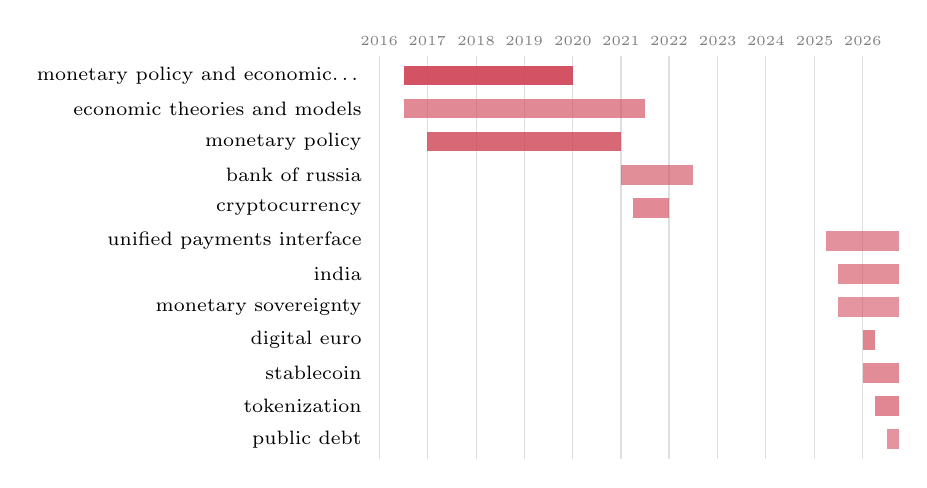
\begin{tikzpicture}[font=\scriptsize, y=-0.42cm]
\draw[gray!25] (0.00,-0.6) -- (0.00,11.60); \node[gray, above, font=\tiny] at (0.00,-0.6) {2016};
\draw[gray!25] (0.61,-0.6) -- (0.61,11.60); \node[gray, above, font=\tiny] at (0.61,-0.6) {2017};
\draw[gray!25] (1.23,-0.6) -- (1.23,11.60); \node[gray, above, font=\tiny] at (1.23,-0.6) {2018};
\draw[gray!25] (1.84,-0.6) -- (1.84,11.60); \node[gray, above, font=\tiny] at (1.84,-0.6) {2019};
\draw[gray!25] (2.46,-0.6) -- (2.46,11.60); \node[gray, above, font=\tiny] at (2.46,-0.6) {2020};
\draw[gray!25] (3.07,-0.6) -- (3.07,11.60); \node[gray, above, font=\tiny] at (3.07,-0.6) {2021};
\draw[gray!25] (3.68,-0.6) -- (3.68,11.60); \node[gray, above, font=\tiny] at (3.68,-0.6) {2022};
\draw[gray!25] (4.30,-0.6) -- (4.30,11.60); \node[gray, above, font=\tiny] at (4.30,-0.6) {2023};
\draw[gray!25] (4.91,-0.6) -- (4.91,11.60); \node[gray, above, font=\tiny] at (4.91,-0.6) {2024};
\draw[gray!25] (5.53,-0.6) -- (5.53,11.60); \node[gray, above, font=\tiny] at (5.53,-0.6) {2025};
\draw[gray!25] (6.14,-0.6) -- (6.14,11.60); \node[gray, above, font=\tiny] at (6.14,-0.6) {2026};
\node[anchor=east] at (-0.1,0) {monetary policy and economic\dots{}};
\fill[c2, opacity=0.95] (0.31,-0.3) rectangle (2.46,0.3);
\node[anchor=east] at (-0.1,1) {economic theories and models};
\fill[c2, opacity=0.65] (0.31,0.7) rectangle (3.38,1.3);
\node[anchor=east] at (-0.1,2) {monetary policy};
\fill[c2, opacity=0.83] (0.61,1.7) rectangle (3.07,2.3);
\node[anchor=east] at (-0.1,3) {bank of russia};
\fill[c2, opacity=0.62] (3.07,2.7) rectangle (3.99,3.3);
\node[anchor=east] at (-0.1,4) {cryptocurrency};
\fill[c2, opacity=0.65] (3.22,3.7) rectangle (3.68,4.3);
\node[anchor=east] at (-0.1,5) {unified payments interface};
\fill[c2, opacity=0.60] (5.68,4.7) rectangle (6.60,5.3);
\node[anchor=east] at (-0.1,6) {india};
\fill[c2, opacity=0.61] (5.83,5.7) rectangle (6.60,6.3);
\node[anchor=east] at (-0.1,7) {monetary sovereignty};
\fill[c2, opacity=0.58] (5.83,6.7) rectangle (6.60,7.3);
\node[anchor=east] at (-0.1,8) {digital euro};
\fill[c2, opacity=0.68] (6.14,7.7) rectangle (6.29,8.3);
\node[anchor=east] at (-0.1,9) {stablecoin};
\fill[c2, opacity=0.63] (6.14,8.7) rectangle (6.60,9.3);
\node[anchor=east] at (-0.1,10) {tokenization};
\fill[c2, opacity=0.66] (6.29,9.7) rectangle (6.60,10.3);
\node[anchor=east] at (-0.1,11) {public debt};
\fill[c2, opacity=0.59] (6.45,10.7) rectangle (6.60,11.3);
\end{tikzpicture}\\[2pt]
\small \alert{Reading}: early bursts on monetary policy and economic impact, economic theories and models, monetary policy; the latest on unified payments interface, india, monetary sovereignty, digital euro.
\method{m:burst}
\note{\textbf{Slide 30} \hfill \textbf{Time: 0:40} \quad clock at the end of the slide: \textbf{20:40} / 25:55\\[3pt]
\textbf{Say:} Kleinberg's algorithm finds when a keyword suddenly becomes frequent, with a cost for entering a burst so that noise is ignored.
Early bursts: monetary policy, economic impact, theory and models. Latest: India and its payment system (UPI), monetary sovereignty, the digital euro. From theory to national projects.}
\end{frame}

% EVENT STUDY ON ATTENTION. Texts dated to the day (71%; dates recorded as 1 January excluded: they
% are year-only dates in disguise), all types.
% Baseline rate lambda over days [-90, -15]: the 15-day gap excludes anticipation (leaks, announced
% dates). Expected E = 15 lambda over [0, 14]; ratio N/E; z = (N - E)/sqrt(E) (Poisson).
% PLACEBO: the same z on 500 random dates (June 2019 - June 2025, seed 7); p = share of random dates
% with a larger z. Needed because attention trends up and comes in waves: the naive test (z > 1.96)
% flags 13% of random dates instead of 2.5%.
% Chart: weekly counts, events as vertical lines numbered like the table, red if p < 0.05.
% Ratios in bold if significant against placebos.
\begin{frame}{Attention around policy events}
\slabel{r:event}
\begin{columns}[c]
\begin{column}{0.48\textwidth}
\begin{tikzpicture}
\begin{axis}[width=\textwidth, height=0.62\textheight, ymin=0, ymax=\ymaxev, xmin=2019, xmax=2026.85,
  xticklabel style={/pgf/number format/1000 sep=, font=\scriptsize}, xtick={2019,...,2026},
  yticklabel style={font=\scriptsize}, ylabel={texts per week}, ylabel style={font=\scriptsize},
  axis lines*=left, clip=false]
\addplot[c1, thin, const plot] coordinates {(2018.997,1) (2019.016,1) (2019.093,2) (2019.112,2) (2019.131,1) (2019.151,3) (2019.170,2) (2019.208,2) (2019.227,2) (2019.246,2) (2019.266,1) (2019.323,5)
  (2019.342,1) (2019.381,2) (2019.400,2) (2019.419,1) (2019.438,1) (2019.496,2) (2019.515,1) (2019.534,2) (2019.553,2) (2019.572,1) (2019.591,1) (2019.611,1)
  (2019.630,2) (2019.649,3) (2019.668,3) (2019.687,1) (2019.706,2) (2019.726,1) (2019.745,4) (2019.764,1) (2019.783,4) (2019.802,3) (2019.821,2) (2019.841,2)
  (2019.860,1) (2019.879,2) (2019.898,3) (2019.917,5) (2019.936,1) (2019.956,2) (2019.994,1) (2020.014,2) (2020.033,1) (2020.052,2) (2020.071,2) (2020.090,1)
  (2020.110,2) (2020.129,2) (2020.148,6) (2020.167,1) (2020.186,4) (2020.244,3) (2020.282,3) (2020.301,1) (2020.320,4) (2020.339,2) (2020.359,1) (2020.378,1)
  (2020.397,1) (2020.416,2) (2020.435,4) (2020.454,2) (2020.474,2) (2020.493,5) (2020.512,2) (2020.550,2) (2020.569,2) (2020.589,1) (2020.608,3) (2020.627,2)
  (2020.646,1) (2020.665,4) (2020.684,4) (2020.704,2) (2020.723,2) (2020.742,7) (2020.761,6) (2020.780,6) (2020.799,6) (2020.819,9) (2020.838,7) (2020.857,1)
  (2020.876,3) (2020.895,5) (2020.914,16) (2020.934,14) (2020.953,2) (2020.972,3) (2020.991,9) (2021.008,1) (2021.047,5) (2021.066,2) (2021.085,6) (2021.104,6)
  (2021.123,1) (2021.142,6) (2021.162,8) (2021.181,1) (2021.200,6) (2021.219,6) (2021.238,8) (2021.257,5) (2021.277,3) (2021.296,5) (2021.315,7) (2021.334,4)
  (2021.353,7) (2021.372,5) (2021.392,10) (2021.411,6) (2021.430,7) (2021.449,6) (2021.468,4) (2021.487,15) (2021.507,2) (2021.526,5) (2021.545,4) (2021.564,5)
  (2021.583,6) (2021.602,3) (2021.621,1) (2021.641,4) (2021.660,8) (2021.679,2) (2021.698,8) (2021.717,5) (2021.736,12) (2021.756,4) (2021.775,3) (2021.794,5)
  (2021.813,2) (2021.832,5) (2021.851,6) (2021.871,5) (2021.890,2) (2021.909,8) (2021.928,6) (2021.947,3) (2021.966,2) (2021.986,9) (2022.005,2) (2022.025,3)
  (2022.044,5) (2022.063,3) (2022.082,7) (2022.101,4) (2022.120,6) (2022.140,3) (2022.159,13) (2022.178,1) (2022.197,3) (2022.216,6) (2022.235,9) (2022.255,2)
  (2022.274,3) (2022.293,6) (2022.312,9) (2022.331,3) (2022.350,3) (2022.370,6) (2022.389,6) (2022.408,14) (2022.427,4) (2022.446,7) (2022.465,5) (2022.485,17)
  (2022.504,3) (2022.523,6) (2022.542,2) (2022.561,2) (2022.580,8) (2022.600,3) (2022.619,10) (2022.638,10) (2022.657,15) (2022.676,6) (2022.695,1) (2022.715,1)
  (2022.734,17) (2022.753,3) (2022.772,6) (2022.791,3) (2022.810,2) (2022.830,8) (2022.849,6) (2022.868,7) (2022.887,3) (2022.906,14) (2022.925,4) (2022.945,3)
  (2022.964,6) (2022.983,15) (2023.003,4) (2023.022,3) (2023.041,5) (2023.060,4) (2023.079,10) (2023.099,4) (2023.118,3) (2023.137,6) (2023.156,20) (2023.175,8)
  (2023.214,3) (2023.233,16) (2023.252,5) (2023.271,7) (2023.290,5) (2023.309,12) (2023.329,10) (2023.348,5) (2023.367,12) (2023.386,7) (2023.405,10) (2023.424,7)
  (2023.444,8) (2023.463,11) (2023.482,22) (2023.501,7) (2023.520,6) (2023.539,7) (2023.559,4) (2023.578,9) (2023.597,2) (2023.616,7) (2023.635,7) (2023.654,25)
  (2023.674,10) (2023.693,8) (2023.712,5) (2023.731,17) (2023.750,4) (2023.769,7) (2023.789,40) (2023.808,19) (2023.827,12) (2023.846,6) (2023.865,6) (2023.884,6)
  (2023.903,24) (2023.923,9) (2023.942,5) (2023.961,13) (2023.980,19) (2024.000,8) (2024.019,4) (2024.038,8) (2024.057,8) (2024.077,11) (2024.096,8) (2024.115,25)
  (2024.134,4) (2024.153,11) (2024.172,13) (2024.192,4) (2024.211,10) (2024.230,8) (2024.249,11) (2024.268,9) (2024.287,8) (2024.307,11) (2024.326,16) (2024.345,5)
  (2024.364,5) (2024.383,8) (2024.402,22) (2024.422,10) (2024.441,6) (2024.460,11) (2024.479,19) (2024.498,12) (2024.517,8) (2024.537,6) (2024.556,5) (2024.575,8)
  (2024.594,4) (2024.613,7) (2024.632,4) (2024.652,15) (2024.671,11) (2024.690,8) (2024.709,9) (2024.728,10) (2024.747,16) (2024.767,8) (2024.786,14) (2024.805,11)
  (2024.824,15) (2024.843,7) (2024.862,9) (2024.882,6) (2024.901,20) (2024.920,13) (2024.939,14) (2024.958,2) (2024.977,6) (2024.997,15) (2025.014,4) (2025.033,13)
  (2025.052,10) (2025.071,17) (2025.090,6) (2025.110,7) (2025.129,9) (2025.148,24) (2025.167,6) (2025.186,8) (2025.205,7) (2025.225,4) (2025.244,15) (2025.263,13)
  (2025.282,5) (2025.301,11) (2025.320,15) (2025.339,8) (2025.359,12) (2025.378,6) (2025.397,24) (2025.416,11) (2025.435,9) (2025.454,12) (2025.474,12) (2025.493,22)
  (2025.512,10) (2025.531,10) (2025.550,6) (2025.569,11) (2025.589,7) (2025.608,6) (2025.627,14) (2025.646,12) (2025.665,16) (2025.684,4) (2025.704,6) (2025.723,11)
  (2025.742,27) (2025.761,13) (2025.780,18) (2025.799,10) (2025.819,47) (2025.838,13) (2025.857,15) (2025.876,10) (2025.895,21) (2025.914,26) (2025.934,17) (2025.953,18)
  (2025.972,15) (2025.991,40) (2026.011,11) (2026.030,8) (2026.049,7) (2026.068,20) (2026.088,15) (2026.107,12) (2026.126,24) (2026.145,30) (2026.164,13) (2026.183,21)
  (2026.203,9) (2026.222,14) (2026.241,30) (2026.260,15) (2026.279,19) (2026.298,13) (2026.318,23) (2026.337,18) (2026.356,22) (2026.375,12) (2026.394,27) (2026.413,30)
  (2026.433,16) (2026.452,31) (2026.471,15) (2026.490,31) (2026.509,21) (2026.528,16) (2026.548,12) (2026.567,23) (2026.586,15) (2026.605,15) (2026.624,20) (2026.643,15)
  (2026.663,34) (2026.682,15) (2026.701,8) (2026.720,12) (2026.739,22) (2026.758,20) (2026.816,2)};
\draw[gray, thin] (axis cs:2019.460,0) -- (axis cs:2019.460,\ymaxev) node[above, font=\scriptsize, inner sep=1pt] {1};
\draw[c2, thin] (axis cs:2020.753,0) -- (axis cs:2020.753,0.9*\ymaxev) node[above, font=\scriptsize, inner sep=1pt] {2};
\draw[c2, thin] (axis cs:2020.802,0) -- (axis cs:2020.802,\ymaxev) node[above, font=\scriptsize, inner sep=1pt] {3};
\draw[gray, thin] (axis cs:2021.531,0) -- (axis cs:2021.531,0.9*\ymaxev) node[above, font=\scriptsize, inner sep=1pt] {4};
\draw[gray, thin] (axis cs:2021.813,0) -- (axis cs:2021.813,\ymaxev) node[above, font=\scriptsize, inner sep=1pt] {5};
\draw[gray, thin] (axis cs:2022.052,0) -- (axis cs:2022.052,0.9*\ymaxev) node[above, font=\scriptsize, inner sep=1pt] {6};
\draw[gray, thin] (axis cs:2022.183,0) -- (axis cs:2022.183,\ymaxev) node[above, font=\scriptsize, inner sep=1pt] {7};
\draw[gray, thin] (axis cs:2022.832,0) -- (axis cs:2022.832,0.9*\ymaxev) node[above, font=\scriptsize, inner sep=1pt] {8};
\draw[gray, thin] (axis cs:2023.101,0) -- (axis cs:2023.101,\ymaxev) node[above, font=\scriptsize, inner sep=1pt] {9};
\draw[c2, thin] (axis cs:2023.487,0) -- (axis cs:2023.487,0.9*\ymaxev) node[above, font=\scriptsize, inner sep=1pt] {10};
\draw[c2, thin] (axis cs:2023.794,0) -- (axis cs:2023.794,\ymaxev) node[above, font=\scriptsize, inner sep=1pt] {11};
\draw[gray, thin] (axis cs:2025.060,0) -- (axis cs:2025.060,0.9*\ymaxev) node[above, font=\scriptsize, inner sep=1pt] {12};
\end{axis}
\end{tikzpicture}
\end{column}
\begin{column}{0.5\textwidth}\tiny
\setlength{\tabcolsep}{2.5pt}
\begin{tabular}{@{}rlp{0.52\linewidth}rrr@{}}\toprule
 & \textbf{Date} & \textbf{Event} & \textbf{Ratio} & $z$ & $p$\\\midrule
1 & Jun 2019 & Facebook announces Libra & 0.3 & -1.3 & 0.83 \\
2 & Oct 2020 & ECB digital euro report & \textbf{2.9} & +4.0 & 0.01 \\
3 & Oct 2020 & Bahamas launches Sand Dollar & \textbf{3.0} & +4.7 & 0.01 \\
4 & Jul 2021 & ECB investigation phase & 0.5 & -1.9 & 0.93 \\
5 & Oct 2021 & Nigeria launches eNaira & 0.8 & -0.7 & 0.69 \\
6 & Jan 2022 & Fed CBDC discussion paper & 1.4 & +1.2 & 0.24 \\
7 & Mar 2022 & US order on digital assets & 0.6 & -1.3 & 0.84 \\
8 & Nov 2022 & India e-rupee pilot & 1.0 & -0.2 & 0.55 \\
9 & Feb 2023 & UK digital pound consultation & 0.7 & -1.0 & 0.76 \\
10 & Jun 2023 & EU digital euro bill & \textbf{1.7} & +2.9 & 0.05 \\
11 & Oct 2023 & ECB preparation phase & \textbf{3.3} & +10.0 & 0.00 \\
12 & Jan 2025 & US order banning a US CBDC & 1.2 & +0.9 & 0.29 \\
\bottomrule\end{tabular}\\[3pt]
\scriptsize Texts in the 15 days after the event vs.\ the rate of the 3 months before. $p$ = share of 500 random dates with a larger $z$ (the naive test flags 13\% of them).\\[2pt]
\alert{Reading}: 4 of 12 events beat 95\% of placebo dates; strongest: ECB preparation phase, Bahamas launches Sand Dollar.
\end{column}
\end{columns}
\method{m:event}
\note{\textbf{Slide 31} \hfill \textbf{Time: 0:50} \quad clock at the end of the slide: \textbf{21:30} / 25:55\\[3pt]
\textbf{Say:} Does writing on CBDCs jump after a policy event? We compare the 15 days after each event with the rate of the 3 months before, and with 500 random dates, because attention grows and comes in waves.
\textbf{4 of 12 events beat 95\% of random dates}: the ECB report and the Sand Dollar launch (October 2020), the EU digital euro bill (June 2023), and the ECB preparation phase (October 2023, three times the usual rate). Libra, the eNaira, the US orders do not.
Red lines on the chart are the significant events.}
\end{frame}

% DIFFERENCE-IN-DIFFERENCES. Treatment: texts about Russia or in Russian (regex: russia, ruble,
% rouble, CBR, Cyrillic forms), exposed to the 2022 sanctions; control: all other texts. Years
% 2020-2026, reference year 2021 (last full year before the invasion of February 2022).
% Linear probability model (OLS on a 0/1 outcome), robust HC1 SEs: chosen over a logit because the
% interaction coefficients are directly in points. Event-study form (one gamma per year, chart) and
% pooled form (one gamma for t > 2021, table).
% Checks: pre-trend (only 2020 is available: stated as a limit) and placebo outcomes: the table shows
% EVERY motivation, so the audience sees that three others also move. Hence "consistent with", not proof.
% Table sorted by effect, bold if CI excludes 0.
\begin{frame}{The 2022 sanctions: did geopolitics enter the discussion?}
\slabel{r:did}
\begin{columns}[T]
\begin{column}{0.5\textwidth}
\begin{tikzpicture}
\begin{axis}[width=\textwidth, height=0.6\textheight, xtick={2020,...,2026}, xticklabel style={/pgf/number format/1000 sep=, font=\scriptsize},
  yticklabel style={font=\scriptsize}, ylabel={gap, points}, ylabel style={font=\scriptsize}, axis lines*=left, ymajorgrids,
  extra x ticks={2021.5}, extra x tick labels={}, extra x tick style={grid=major, major grid style={c2, dashed}}]
\addplot[c1, thick, mark=*, mark size=1.5pt, error bars/.cd, y dir=both, y explicit] coordinates {(2020,5.2) +- (0,16.1) (2021,0.0) +- (0,0.0) (2022,6.5) +- (0,11.5) (2023,10.1) +- (0,9.5) (2024,12.6) +- (0,9.6) (2025,12.2) +- (0,9.7) (2026,16.5) +- (0,9.7)};
\draw[gray] (axis cs:2020,0) -- (axis cs:2026,0);
\end{axis}
\end{tikzpicture}\\
\scriptsize Gap in the share stating \emph{geopolitics and sanctions}: texts about Russia (or in Russian) minus the others, relative to 2021; 95\% CI.
\end{column}
\begin{column}{0.48\textwidth}\scriptsize
756 texts about Russia among 3,772 (2020--2026). Pooled effect after 2021, every motivation:\\[2pt]
\begin{tabular}{@{}p{0.6\linewidth}l@{}}\toprule
\textbf{Motivation} & \textbf{DiD, points}\\\midrule
Geopolitics and sanctions & \textbf{+11.6} \tiny[+5, +18] \\
Cross-border payments & +8.1 \tiny[-2, +18] \\
Payment efficiency & +7.1 \tiny[-1, +15] \\
Decline of cash & +2.8 \tiny[-2, +8] \\
Privacy and surveillance & -4.0 \tiny[-11, +3] \\
Financial inclusion & \textbf{-6.7} \tiny[-13, -0] \\
Monetary sovereignty & -8.7 \tiny[-18, +1] \\
Technology (DLT, programmability) & -10.0 \tiny[-21, +1] \\
Monetary policy & \textbf{-12.0} \tiny[-24, -0] \\
Financial stability & \textbf{-12.6} \tiny[-25, -1] \\
\bottomrule\end{tabular}\\[4pt]
\small \alert{Reading}: geopolitics rises by $+11.6$ points [+5, +18] more in texts about Russia, and the gap widens each year. But 3 other motivations shift too: \alert{consistent with} a sanctions effect, not proof.
\end{column}
\end{columns}
\method{m:did}
\note{\textbf{Slide 32} \hfill \textbf{Time: 1:00} \quad clock at the end of the slide: \textbf{22:30} / 25:55\\[3pt]
\textbf{Say:} After the 2022 sanctions, did geopolitics enter the discussion? We compare texts about Russia with the others, before and after 2021.
Geopolitics and sanctions rises by \textbf{11.6 points more} in texts about Russia [+5, +18], and the gap widens every year.
But other motivations move too (monetary policy, financial stability, inclusion), and we have only one clean year before (2020). So: \textbf{consistent with} a sanctions effect, not proof.}
\end{frame}

% =====================================================================
\section{The discussion and its environment}

% SYNTHESIS. Rows = results of the previous sections, columns = the three periods: the table answers
% the second half of the research question (alignment with the policy environment) without new
% computation. Events in bold if attention reacted. Tone: research / central banks. Stance: LLM
% shares (levels inflated, read the changes). Texts per year: mean per period.
% Tiny font is acceptable here: the bullets underneath carry the message.
\begin{frame}{Putting it together, period by period}
\slabel{r:syn}
\scriptsize
\setlength{\tabcolsep}{4pt}
\tiny
\begin{tabular}{@{}p{0.19\textwidth}p{0.25\textwidth}p{0.25\textwidth}p{0.26\textwidth}@{}}\toprule
 & \textbf{2014--2019} & \textbf{2020--2022} & \textbf{2023--2026}\\\midrule
Policy events (bold: attention reacts) & Facebook announces Libra & \textbf{ECB digital euro report}; \textbf{Bahamas launches Sand Dollar}; ECB investigation phase; Nigeria launches eNaira; Fed CBDC discussion paper; US order on digital assets; India e-rupee pilot & UK digital pound consultation; \textbf{EU digital euro bill}; \textbf{ECB preparation phase}; US order banning a US CBDC \\
Texts per year & 53 & 324 & 840 \\
Bursting keywords & monetary policy and economic impact, economic theories and models, monetary policy & bank of russia, cryptocurrency & unified payments interface, india, monetary sovereignty \\
Most frequent motivations & monetary policy, financial stability, technology & monetary policy, financial stability, technology & financial stability, technology, monetary policy \\
Net tone (research / central banks) & 0.06 / 0.10 & 0.15 / 0.22 & 0.21 / 0.24 \\
Favourable, LLM (research / central banks) & 26\% / 25\% & 38\% / 54\% & 40\% / 65\% \\
\bottomrule\end{tabular}\\[2pt]
\scriptsize
\begin{itemize}\setlength\itemsep{0pt}
\item \alert{2014--19}: a monetary-policy question, alongside Libra and the decline of cash; few texts, cautious tone.
\item \alert{2020--22}: central bank reports and pilots; the discussion grows and turns favourable.
\item \alert{2023--26}: national projects, sanctions, cross-border payments; the most favourable period.
\end{itemize}
\note{\textbf{Slide 33} \hfill \textbf{Time: 1:00} \quad clock at the end of the slide: \textbf{23:30} / 25:55\\[3pt]
\textbf{Say:} Three periods.
\begin{itemize}
\item 2014--19: a monetary-policy question, alongside Libra and the decline of cash; few texts, cautious tone.
\item 2020--22: central bank reports and pilots; the discussion grows and turns favourable.
\item 2023--26: national projects, sanctions, cross-border payments; the most favourable period.
\end{itemize}
The discussion moves with its environment: more texts, more favourable, new motivations, as projects advance.}
\end{frame}

% CAUSES. The teacher's question, answered in one table: each link, the test, the result, and a
% verdict with a colour (green = timing evidence, red = no effect, amber = consistent with). Links that
% cannot be tested are listed too, to show the limits are known.
\begin{frame}{What we can and cannot say about causes}
\slabel{r:causal}
\footnotesize
\begin{tabular}{@{}p{0.25\textwidth}p{0.27\textwidth}p{0.2\textwidth}p{0.18\textwidth}@{}}\toprule
\textbf{Link} & \textbf{Test} & \textbf{Result} & \textbf{Verdict}\\\midrule
Events $\to$ attention & event study vs.\ placebo dates & 4 of 12 events & \textcolor{c6}{\textbf{timing evidence}}\\
Events $\to$ tone & 180-day windows vs.\ placebo dates & 0 of 12 events & \textcolor{c2}{\textbf{no effect found}}\\
Sanctions $\to$ geopolitics motive & difference-in-differences & $+11.6$ points [+5, +18] & \textcolor{c3}{\textbf{consistent with}}\\
Events $\to$ stance & -- & sample too small around each date & not testable\\
Motivations $\leftrightarrow$ stance & -- & measured in the same texts & association only\\
\bottomrule\end{tabular}\\[8pt]
\small
\begin{itemize}\setlength\itemsep{2pt}
\item The paper stays \alert{descriptive}: it measures changes and shows what moves with them.
\item Explaining \emph{why} economists changed their stance would need other evidence (interviews, authors' careers): hypotheses for further work.
\end{itemize}
\note{\textbf{Slide 34} \hfill \textbf{Time: 0:50} \quad clock at the end of the slide: \textbf{24:20} / 25:55\\[3pt]
\textbf{Say:} What can we say about causes?
Events move attention (4 of 12): timing evidence. Events do not move tone (0 of 12). The sanctions are consistent with the rise of geopolitics, not proof. Events and stance: samples too small around each date. Motivations and stance are measured in the same texts: association only.
So the paper stays descriptive; explaining \emph{why} economists changed their stance would need other evidence, interviews or authors' careers.}
\end{frame}

% =====================================================================
\section{Robustness}

% ROBUSTNESS. One row per specification that removes one possible source of error; columns = the
% headline results of each W (inclusion and monetary policy for Why, tone gap and stance gap for How,
% events for When). The baseline is the first row; the last row drops the economist filter entirely.
% Reading: signs and magnitudes hold in every row.
\begin{frame}{Robustness}
\slabel{r:robust}
\scriptsize
\setlength{\tabcolsep}{4pt}
\begin{tabular}{@{}lrcccrr@{}}\toprule
 & & \multicolumn{2}{c}{\textbf{Why: change, points}} & \textbf{How: tone} & \textbf{How: stance} & \textbf{When}\\
\textbf{Specification} & \textbf{Texts} & \textbf{inclusion} & \textbf{monetary policy} & \textbf{CB -- research} & \textbf{fav.\ CB -- research} & \textbf{events}\\\midrule
Baseline: economists & 4,710 & $+12.3$ \tiny[+8, +15] & $-15.1$ \tiny[-22, -8] & $+0.03$ & $+16$ & 4/12 \\
Main theme only & 3,513 & $+14.9$ \tiny[+10, +18] & $-16.0$ \tiny[-25, -7] & $+0.01$ & $+13$ & 4/12 \\
English only & 3,721 & $+13.7$ \tiny[+9, +16] & $-16.0$ \tiny[-23, -7] & $+0.03$ & $+16$ & 4/12 \\
Journal articles only (research) & 3,171 & $+12.3$ \tiny[+6, +15] & $-16.8$ \tiny[-25, -8] & $+0.01$ & $+11$ & 4/12 \\
Without 2026 (partial year) & 3,547 & $+11.8$ \tiny[+7, +15] & $-15.3$ \tiny[-23, -8] & $+0.03$ & $+15$ & 4/12 \\
High-recall motivation coding & 4,710 & $+15.6$ \tiny[+10, +19] & $-8.8$ \tiny[-16, -2] & $+0.03$ & $+16$ & 4/12 \\
All disciplines (not only economists) & 8,213 & $+13.2$ \tiny[+10, +15] & $-15.0$ \tiny[-21, -9] & $+0.02$ & $+15$ & 4/12 \\
\bottomrule\end{tabular}\\[4pt]
Changes: 2023--26 vs 2014--19, adjusted (logit, 95\% CI). Tone: mean net tone gap. Stance: raw LLM labels, points. Events: $p < 0.05$ against placebo dates.\\[3pt]
\small Signs and orders of magnitude hold in every specification, including when research from every discipline is kept.
\method{m:robust}
\note{\textbf{Slide 35} \hfill \textbf{Time: 0:45} \quad clock at the end of the slide: \textbf{25:05} / 25:55\\[3pt]
\textbf{Say:} We re-ran the headline results seven ways: main theme only, English only, journal articles only, without the partial year 2026, with a high-recall motivation coding, and with research from every discipline.
Signs and orders of magnitude hold everywhere: inclusion $+12$ to $+16$ points, monetary policy $-9$ to $-17$, the same 4 events.}
\end{frame}

% =====================================================================
\section{Conclusion}

% TAKEAWAYS. One bullet per W, each with its number, then the limits in a separate column so they are
% visible, not hidden.
% NOTE: "recall ~ 0.5" here vs 0.41 elsewhere: say 0.4. "One coder (AI-assisted)": a second coder
% (Kenza) has since filled the coding sheet; inter-coder agreement is not on the slides yet.
\begin{frame}{Takeaways and limits}
\begin{columns}[T]
\begin{column}{0.56\textwidth}\footnotesize
\textbf{How economists' discussion of CBDCs evolved}
\begin{itemize}\setlength\itemsep{1pt}
\item \alert{Who:} 4,710 texts; central bank economists write 10\% of the papers but get 48\% of citations.
\item \alert{What:} from monetary policy and design to inclusion and national projects (digital ruble, rupee, e-CNY).
\item \alert{How:} tone and stance become more favourable; research economists stay mostly neutral, central banks advocate.
\item \alert{Why:} rising geopolitics and sanctions ($+12$\,pts), financial inclusion ($+12$\,pts), cross-border payments ($+9$\,pts); falling monetary policy ($-15$\,pts), decline of cash ($-7$\,pts).
\item \alert{When:} 4 of 12 events move attention, 0 of 12 move tone; geopolitics rises after the 2022 sanctions.
\end{itemize}
\end{column}
\begin{column}{0.41\textwidth}\footnotesize
\textbf{Limits}
\begin{itemize}\setlength\itemsep{1pt}
\item Economists identified by field and affiliation, not by training.
\item Motivations: recall $\approx$ 0.5 (lower bounds). Tone: English only. Stance: LLM for changes only.
\item One coder (AI-assisted) for the validation samples.
\item Descriptive: causes stay hypotheses.
\end{itemize}
\end{column}
\end{columns}
\note{\textbf{Slide 36} \hfill \textbf{Time: 0:50} \quad clock at the end of the slide: \textbf{25:55} / 25:55\\[3pt]
\textbf{Say:} To conclude:
\begin{itemize}
\item Who: 4,710 texts; central bank economists write 10\% of papers but get half the citations.
\item What: from monetary policy and design to inclusion and national projects.
\item How: tone and stance become more favourable; researchers stay neutral, central banks advocate.
\item Why: geopolitics, inclusion and cross-border payments rise; monetary policy and cash fall.
\item When: events move attention, not tone; geopolitics rises after the 2022 sanctions.
\end{itemize}
Limits: economists identified by field and employer, not training; motivations are lower bounds; tone in English only; descriptive.
\textbf{Thank you; we are happy to take questions.}}
\end{frame}

% =====================================================================
\appendix
\section*{Methods explained}

% APPENDIX INDEX. Every method slide has the same four parts (Idea, How, Why this tool, Used on), so a
% question can be answered by pointing at the same place on any slide. Clickable table of methods.
\begin{frame}{Methods explained: how to read this appendix}
\small
One slide per tool, each in four parts:
\begin{itemize}
\item \textbf{Idea}: what the tool does, in words.
\item \textbf{How}: the computation, step by step, with its formula.
\item \textbf{Why this tool}: what it solves, and what it was compared with.
\item \textbf{Used on}: links to the result slides.
\end{itemize}
\vspace{4pt}
\scriptsize
\begin{tabular}{@{}llll@{}}\toprule
\textbf{Tool} & \textbf{Slide} & \textbf{Tool} & \textbf{Slide}\\\midrule
Who is an economist & \usedon{m:econ} & Covariate-adjusted logit & \usedon{m:logit}\\
Networks: association strength, Louvain & \usedon{m:net} & Codebook and validation & \usedon{m:codebook}\\
Thematic map (Callon) & \usedon{m:callon} & Tone (FinBERT) & \usedon{m:finbert}\\
Bibliometric laws & \usedon{m:laws} & Stance (reading + LLM) & \usedon{m:stance}\\
Log-odds with Dirichlet prior & \usedon{m:logodds} & Bursts (Kleinberg) & \usedon{m:burst}\\
Sentence embeddings (SBERT) & \usedon{m:sbert} & Event study and placebo & \usedon{m:event}\\
Topic model (BERTopic) & \usedon{m:bertopic} & Tone around events & \usedon{m:tev}\\
Class-based TF-IDF & \usedon{m:ctfidf} & Difference-in-differences & \usedon{m:did}\\
 & & Robustness & \usedon{m:robust}\\
\bottomrule\end{tabular}
\note{\textbf{Slide 37}\\[3pt]
\textbf{Appendix: shown only if asked (0:00 in the budget).} Use this index to jump to the method a question is about.}
\end{frame}

% See step 4. Rules in order: OpenAlex primary-topic field; central bank / IMF / BIS affiliation (regex
% CB_AFFIL); economics venue (regex ECON_VENUE) for records without OpenAlex data.
\begin{frame}{Method: who counts as an economist}
\slabel{m:econ}
\begin{columns}[T]
\begin{column}{0.5\textwidth}\footnotesize
\mhead{Idea}
The course asks how \emph{economists} discuss CBDCs, so each text must be traced to an economist or an economic institution.\\[4pt]
\mhead{How}
\begin{itemize}\setlength\itemsep{1pt}
\item \textbf{Research}: kept if OpenAlex classifies it in \emph{Economics, Econometrics and Finance} (primary topic, from title, abstract, venue, citations), or an author works at a central bank, the IMF or the BIS; without OpenAlex record: an economics venue.
\item \textbf{Institutions}: central bank speeches; documents of central banks and international financial institutions.
\item \textbf{Dropped}: other fields (computer science, law\dots), governments and parliaments, the press.
\end{itemize}
\end{column}
\begin{column}{0.46\textwidth}\footnotesize
\mhead{Why this tool}
Authors' training is not recorded anywhere at scale; the field of the paper and the employer of the author are, and they are what defines a discipline in bibliometrics.\\[4pt]
Speeches are kept as \emph{institutional} voices: written with the bank's economics staff, even when the speaker is not an economist.\\[4pt]
Robustness: results with every discipline kept are on \usedon{r:robust}.\\[6pt]
\mhead{Used on}
\usedon{r:econ}, and every result after it.
\end{column}
\end{columns}
\note{\textbf{Slide 38}\\[3pt]
\textbf{Appendix: shown only if asked (0:00 in the budget).} Key line: training is not recorded at scale; field and employer are what bibliometrics uses. Speeches = institutional voice. With every discipline kept, results hold (robustness).}
\end{frame}

% Weight s_ij = c_ij/(c_i c_j); Louvain on that weight, seed 7, sorted nodes (deterministic). Node area ~
% count (radius ~ sqrt). Edge opacity ~ strength.
\begin{frame}{Method: networks (association strength, Louvain)}
\slabel{m:net}
\begin{columns}[T]
\begin{column}{0.52\textwidth}\footnotesize
\mhead{Idea}
Two items (references, authors, keywords) are linked when they appear in the same paper; groups of tightly linked items are schools, teams or themes.\\[4pt]
\mhead{How}
\begin{enumerate}\setlength\itemsep{1pt}
\item Count $c_{ij}$ = papers where $i$ and $j$ appear together; $c_i$ = papers with $i$.
\item Normalise by \alert{association strength} $s_{ij} = c_{ij} / (c_i c_j)$: the ratio of observed to expected co-occurrence.
\item Cluster with \alert{Louvain}: move nodes between groups while the modularity
$Q = \frac{1}{2m}\sum_{ij}\big[s_{ij} - \frac{k_ik_j}{2m}\big]\delta(g_i,g_j)$ rises.
\item Draw: force-directed layout; size $\propto\sqrt{c_i}$.
\end{enumerate}
\end{column}
\begin{column}{0.44\textwidth}\footnotesize
\mhead{Why this tool}
Raw counts favour popular items: two classics are co-cited often by chance. Association strength removes this (van Eck \& Waltman, 2009); it is VOSviewer's default.\\[3pt]
Louvain is fast and needs no number of clusters; $Q$ tells how clear the grouping is.\\[3pt]
\textbf{Co-citation} (references cited together) shows the intellectual base; \textbf{co-authorship} shows teams.\\[6pt]
\mhead{Used on}
\usedon{r:cocit}, \usedon{r:coauth}, \usedon{r:thematic}.
\end{column}
\end{columns}
\note{\textbf{Slide 39}\\[3pt]
\textbf{Appendix: shown only if asked (0:00 in the budget).} Why association strength: raw counts link popular items by chance. Why Louvain: fast, no number of clusters to choose; $Q$ says how clear the grouping is (0.10: weak).}
\end{frame}

% Equivalence index e_ij = c_ij^2/(c_i c_j); factors 10 and 100 are Callon's scaling conventions;
% quadrants at medians.
\begin{frame}{Method: thematic map (Callon)}
\slabel{m:callon}
\begin{columns}[T]
\begin{column}{0.52\textwidth}\footnotesize
\mhead{Idea}
Place each cluster of keywords on two axes: how much it is linked to the rest of the field, and how developed it is inside.\\[4pt]
\mhead{How}
With the equivalence index $e_{ij} = c_{ij}^2 / (c_i c_j)$:
\[ \text{centrality} = 10\!\!\sum_{i\in C,\,j\notin C}\!\! e_{ij}, \qquad \text{density} = \frac{100}{|C|}\!\sum_{i,j\in C}\! e_{ij} \]
Quadrants, split at the medians:
\begin{itemize}\setlength\itemsep{0pt}
\item \textbf{motor}: central and dense; \textbf{basic}: central, loose;
\item \textbf{niche}: dense, isolated; \textbf{emerging or declining}: neither.
\end{itemize}
\end{column}
\begin{column}{0.44\textwidth}\footnotesize
\mhead{Why this tool}
A keyword list says what is frequent; the map says what \emph{structures} the field. It is the standard tool of science mapping (Callon et al.\ 1991; Cobo et al.\ 2011; bibliometrix).\\[3pt]
Limit: keywords are partly machine-assigned, so the topic model (meaning-based) is used alongside.\\[6pt]
\mhead{Used on}
\usedon{r:thematic}.
\end{column}
\end{columns}
\note{\textbf{Slide 40}\\[3pt]
\textbf{Appendix: shown only if asked (0:00 in the budget).} Motor = central and dense; basic = central, loose; niche = dense, isolated; emerging or declining = neither. Limit: keywords are partly machine-assigned, hence the topic model alongside.}
\end{frame}

% Growth: compound annual rate. Lotka beta by least squares on log-log. Bradford: three zones of 1/3.
\begin{frame}{Method: bibliometric laws}
\slabel{m:laws}
\begin{columns}[T]
\begin{column}{0.52\textwidth}\footnotesize
\mhead{Idea}
Three regularities describe the shape of any scientific field: how fast it grows, how output is spread among authors, and among journals.\\[4pt]
\mhead{How}
\begin{itemize}\setlength\itemsep{1pt}
\item \textbf{Growth}: compound annual rate $g = (N_{y_1}/N_{y_0})^{1/(y_1-y_0)} - 1$.
\item \textbf{Lotka}: share of authors with $n$ papers $f(n) \propto n^{-\beta}$; $\beta$ fitted on the log-log counts ($\beta \approx 2$ in mature fields).
\item \textbf{Bradford}: sort sources by output, cut in three zones holding $\nicefrac{1}{3}$ of papers each; the first zone is the core.
\end{itemize}
\end{column}
\begin{column}{0.44\textwidth}\footnotesize
\mhead{Why this tool}
They situate the field: a high growth rate and a large $\beta$ (most authors write once) mean a young, open field around a small core of outlets.\\[3pt]
They are the descriptive baseline of every bibliometric review, so our numbers can be compared with the earlier reviews.\\[6pt]
\mhead{Used on}
\usedon{r:growth}, \usedon{r:research}.
\end{column}
\end{columns}
\note{\textbf{Slide 41}\\[3pt]
\textbf{Appendix: shown only if asked (0:00 in the budget).} Growth 60\%/year; Lotka exponent 3.3 (most authors write once); Bradford zones 21 : 310 : 1,148 (dispersed field).}
\end{frame}

% alpha_0 = 500, alpha_w proportional to corpus frequency; vocabulary >= 20 occurrences.
\begin{frame}{Method: distinctive words (log-odds with Dirichlet prior)}
\slabel{m:logodds}
\begin{columns}[T]
\begin{column}{0.54\textwidth}\footnotesize
\mhead{Idea}
Which words does one group use \emph{more} than the other, once chance is accounted for?\\[4pt]
\mhead{How}
For word $w$, group $i$ vs.\ the other group $j$, with counts $y$, totals $n$, and a prior $\alpha_w = \alpha_0 \times$ (corpus frequency of $w$):
\[\delta_w = \log\frac{y_{iw}+\alpha_w}{n_i+\alpha_0-y_{iw}-\alpha_w} - \log\frac{y_{jw}+\alpha_w}{n_j+\alpha_0-y_{jw}-\alpha_w}\]
\[ z_w = \delta_w \Big/ \sqrt{\tfrac{1}{y_{iw}+\alpha_w}+\tfrac{1}{y_{jw}+\alpha_w}} \]
Words are ranked by $z_w$.
\end{column}
\begin{column}{0.42\textwidth}\footnotesize
\mhead{Why this tool}
Plain frequencies list words everyone uses; TF-IDF or raw log-ratios are dominated by rare words (a word used twice by one group gets an infinite ratio). The prior \alert{shrinks} rare words towards zero and the $z$-score accounts for uncertainty (Monroe, Colaresi \& Quinn, 2008).\\[6pt]
\mhead{Used on}
\usedon{r:logodds}.
\end{column}
\end{columns}
\note{\textbf{Slide 42}\\[3pt]
\textbf{Appendix: shown only if asked (0:00 in the budget).} The prior adds pseudo-counts proportional to each word's overall frequency: rare words are pulled to zero; the $z$-score accounts for uncertainty.}
\end{frame}

% Model paraphrase-multilingual-MiniLM-L12-v2, 384 dimensions, normalised vectors (cosine).
\begin{frame}{Method: sentence embeddings (SBERT)}
\slabel{m:sbert}
\begin{columns}[T]
\begin{column}{0.52\textwidth}\footnotesize
\mhead{Idea}
Turn each text into a vector of 384 numbers such that texts with similar \emph{meaning} get close vectors, whatever their words or language.\\[4pt]
\mhead{How}
\begin{itemize}\setlength\itemsep{1pt}
\item A transformer network reads title + abstract (or opening) and averages its word representations into one vector $\mathbf{e}_t$.
\item Model: \texttt{paraphrase-multilingual-MiniLM-L12-v2}, trained so that translations and paraphrases land together (50+ languages).
\item Similarity: cosine $\cos(\mathbf{e}_s,\mathbf{e}_t) = \frac{\mathbf{e}_s\cdot\mathbf{e}_t}{\|\mathbf{e}_s\|\|\mathbf{e}_t\|}$.
\end{itemize}
\end{column}
\begin{column}{0.44\textwidth}\footnotesize
\mhead{Why this tool}
Keywords and word counts treat ``digital ruble'' and its Russian original (\emph{tsifrovoy rubl'}) as unrelated; embeddings do not. With 79\% English and many Russian texts, this is what makes a single topic model possible.\\[3pt]
Tested also as a motivation coder (similarity to prototypes): it lost to the codebook (\usedon{r:coders}).\\[6pt]
\mhead{Used on}
\usedon{r:topics}.
\end{column}
\end{columns}
\note{\textbf{Slide 43}\\[3pt]
\textbf{Appendix: shown only if asked (0:00 in the budget).} Why: keywords treat ``digital ruble'' and \emph{tsifrovoy rubl'} as unrelated; embeddings do not. Tested as a motivation coder too: lost to the codebook.}
\end{frame}

% UMAP 15 neighbours / 5 dims / min_dist 0 / cosine / seed 42; HDBSCAN min size 40, min_samples 10,
% leaf; outliers reassigned by embedding similarity.
\begin{frame}{Method: topic model (BERTopic)}
\slabel{m:bertopic}
\begin{columns}[T]
\begin{column}{0.52\textwidth}\footnotesize
\mhead{Idea}
Find groups of texts about the same subject, without fixing the subjects in advance.\\[4pt]
\mhead{How}
\begin{enumerate}\setlength\itemsep{1pt}
\item \textbf{Embed} each text (SBERT).
\item \textbf{Reduce} 384 dimensions to 5 with \alert{UMAP}, which keeps neighbours together.
\item \textbf{Cluster} with \alert{HDBSCAN}: dense regions become topics (at least 40 texts; leaf selection, which favours fine topics over one large blob); texts in no dense region are outliers, then assigned to the nearest topic.
\item \textbf{Label} each topic by its c-TF-IDF terms (\usedon{m:ctfidf}).
\end{enumerate}
\end{column}
\begin{column}{0.44\textwidth}\footnotesize
\mhead{Why this tool}
LDA and STM count words, one language at a time, and need the number of topics. BERTopic works on meaning, across languages, and finds the number itself (Grootendorst, 2022).\\[3pt]
The covariate part of STM is kept: topic shares are adjusted for period, actor and language (\usedon{m:logit}).\\[6pt]
\mhead{Used on}
\usedon{r:topics}.
\end{column}
\end{columns}
\note{\textbf{Slide 44}\\[3pt]
\textbf{Appendix: shown only if asked (0:00 in the budget).} Why leaf selection: the default merged half the corpus into one topic. Why 40: smallest topic still large enough to compute shares by period.}
\end{frame}

% Words in more than 15% of texts removed (max_df 0.15: money, policy, financial...), min_df 5
% (10 for periods); 5-6 terms per class.
\begin{frame}{Method: class-based TF-IDF (c-TF-IDF)}
\slabel{m:ctfidf}
\begin{columns}[T]
\begin{column}{0.52\textwidth}\footnotesize
\mhead{Idea}
Which words characterise a class of texts (a topic, or a period) compared with all the others?\\[4pt]
\mhead{How}
Merge the texts of each class $c$ into one document; for term $t$:
\[ W_{t,c} = \frac{\text{tf}_{t,c}}{|c|}\;\log\!\Big(1 + \frac{A}{f_t}\Big) \]
$\text{tf}_{t,c}$ = count of $t$ in class $c$, $|c|$ = words in $c$, $A$ = average words per class, $f_t$ = count of $t$ in all classes. Words in more than 15\% of texts and generic words are removed.
\end{column}
\begin{column}{0.44\textwidth}\footnotesize
\mhead{Why this tool}
Ordinary TF-IDF scores words within one document; here the unit is a whole class. A frequent word in one class but rare elsewhere scores high: it is what is \emph{new} or \emph{specific}.\\[3pt]
Periods as classes answer ``when'': which vocabulary appears in each period.\\[6pt]
\mhead{Used on}
\usedon{r:topics} (topic labels), \usedon{r:evo} (periods).
\end{column}
\end{columns}
\note{\textbf{Slide 45}\\[3pt]
\textbf{Appendix: shown only if asked (0:00 in the budget).} Whole topic (or period) treated as one document: a word frequent in one class and rare elsewhere scores high.}
\end{frame}

% Covariates: period (reference 2014-19), actor (reference research), English. AME by predicting every
% text in both periods. 400 coefficient draws for the CI.
\begin{frame}{Method: covariate-adjusted logit}
\slabel{m:logit}
\begin{columns}[T]
\begin{column}{0.52\textwidth}\footnotesize
\mhead{Idea}
A raw change between periods can come from a change in \emph{who} writes (more central banks, more Russian texts). Compare like with like.\\[4pt]
\mhead{How}
For each outcome $y_t \in\{0,1\}$ (a motivation, a topic):
\[ P(y_t=1) = \Lambda\big(a + b_{\text{period}} + c_{\text{actor}} + e\cdot\text{English}\big) \]
\begin{itemize}\setlength\itemsep{1pt}
\item \textbf{Average marginal effect}: predict every text in 2023--26, then in 2014--19, average the difference (points).
\item 95\% CI: robust (HC1) standard errors; coefficients drawn 400 times from their estimated distribution.
\end{itemize}
\end{column}
\begin{column}{0.44\textwidth}\footnotesize
\mhead{Why this tool}
It is the ``prevalence'' model of a structural topic model (Roberts et al., 2014), applied to any coded outcome. Marginal effects are read in percentage points, unlike log-odds coefficients.\\[6pt]
\mhead{Used on}
\usedon{r:motives}, \usedon{r:topics}, \usedon{r:robust}.
\end{column}
\end{columns}
\note{\textbf{Slide 46}\\[3pt]
\textbf{Appendix: shown only if asked (0:00 in the budget).} Why: the mix of authors changes over time; the marginal effect compares the same texts in two periods, in points.}
\end{frame}

% Development 100 texts, test 74 (50 by economists), unit = text x motivation (500 pairs).
\begin{frame}{Method: codebook and validation}
\slabel{m:codebook}
\begin{columns}[T]
\begin{column}{0.52\textwidth}\footnotesize
\mhead{Idea}
Write down, for each of 10 motivations, the phrases authors use to state it; flag a text when its introduction contains one.\\[4pt]
\mhead{How}
\begin{enumerate}\setlength\itemsep{1pt}
\item Read 100 introductions (\textbf{development set}); write regular expressions in 7 languages.
\item Code 74 \emph{other} texts by reading (\textbf{test set}), never used for tuning; scores on the 50 written by economists.
\item Compare: precision $=\frac{TP}{TP+FP}$, recall $=\frac{TP}{TP+FN}$, Cohen's
$\kappa = \frac{p_o-p_e}{1-p_e}$ (agreement beyond chance).
\end{enumerate}
\end{column}
\begin{column}{0.44\textwidth}\footnotesize
\mhead{Why this tool}
Motivations need reading; a codebook makes the reading explicit, reproducible and checkable.\\[3pt]
Five machine coders were tested on the same texts (SBERT $\times$ 2, NLI mDeBERTa, Qwen2.5 3B and 7B): see \usedon{r:coders}.\\[3pt]
High precision, recall $\approx 0.5$: shares are lower bounds; changes are robust (\usedon{r:coders}).\\[6pt]
\mhead{Used on}
\usedon{r:codebook}, \usedon{r:motives}, \usedon{r:coders}.
\end{column}
\end{columns}
\note{\textbf{Slide 47}\\[3pt]
\textbf{Appendix: shown only if asked (0:00 in the budget).} Precision = share of codebook flags that are right; recall = share of read motivations found; kappa = agreement beyond chance.}
\end{frame}

% ProsusAI/finbert; up to 30 CBDC sentences per text; text-level averaging gives each text equal weight.
\begin{frame}{Method: tone (FinBERT)}
\slabel{m:finbert}
\begin{columns}[T]
\begin{column}{0.52\textwidth}\footnotesize
\mhead{Idea}
Measure how positive or negative the sentences \emph{about CBDCs} are.\\[4pt]
\mhead{How}
\begin{enumerate}\setlength\itemsep{1pt}
\item Keep the English sentences that name a CBDC (same term list as the filter).
\item FinBERT (a BERT model trained on financial news) gives $P(+), P(0), P(-)$ for each sentence.
\item Sentence tone $= P(+) - P(-) \in[-1,1]$; averaged per text, then per group and year.
\item Validation: 90 sentences from economists' texts read blind; $\kappa = 0.52$ (all 0.53).
\end{enumerate}
\end{column}
\begin{column}{0.44\textwidth}\footnotesize
\mhead{Why this tool}
Dictionary methods (Loughran--McDonald) miss context (``not risky''); general sentiment models misread finance (``liability'' is not negative). FinBERT is the standard for economic text (Araci, 2019).\\[3pt]
Scoring only CBDC sentences isolates the tone \emph{about CBDCs}, not about the economy.\\[3pt]
Limit: it sees tone in neutral sentences, so compare groups and years, not levels.\\[6pt]
\mhead{Used on}
\usedon{r:tone}, \usedon{r:tev}.
\end{column}
\end{columns}
\note{\textbf{Slide 48}\\[3pt]
\textbf{Appendix: shown only if asked (0:00 in the budget).} Why FinBERT: dictionaries miss context (``not risky''); general sentiment models misread finance (``liability'' is not negative). Limit: sees tone in neutral sentences, so compare, do not read levels.}
\end{frame}

% Qwen2.5-7B-Instruct 4-bit via mlx, one-word answer; up to 100 texts per actor x period.
\begin{frame}{Method: stance (reading + local language model)}
\slabel{m:stance}
\begin{columns}[T]
\begin{column}{0.52\textwidth}\footnotesize
\mhead{Idea}
Tone is about words; stance is about the \emph{author's position}: favourable, neutral or critical towards issuing a CBDC.\\[4pt]
\mhead{How}
\begin{itemize}\setlength\itemsep{1pt}
\item \textbf{Levels}: texts read by hand per actor; share with a \alert{Wilson} interval $\frac{\hat p + \frac{z^2}{2n} \pm z\sqrt{\frac{\hat p(1-\hat p)}{n}+\frac{z^2}{4n^2}}}{1+z^2/n}$.
\item \textbf{Changes}: Qwen2.5 7B, run locally, labels a random sample of up to 100 texts per actor $\times$ period; change $= \hat p_{\text{late}} - \hat p_{\text{early}}$, CI $\pm 1.96\sqrt{\sum \hat p(1-\hat p)/n}$.
\end{itemize}
\end{column}
\begin{column}{0.44\textwidth}\footnotesize
\mhead{Why this tool}
Stance needs understanding of the argument: only a language model can do it at scale. Four coders were tested (\usedon{b:stance}); the LLM is best ($\kappa = 0.45$) but over-calls ``favourable''.\\[3pt]
A constant bias cancels in a difference: so the LLM gives \emph{changes}, reading gives \emph{levels}.\\[6pt]
\mhead{Used on}
\usedon{r:stance}, \usedon{r:syn}.
\end{column}
\end{columns}
\note{\textbf{Slide 49}\\[3pt]
\textbf{Appendix: shown only if asked (0:00 in the budget).} Levels from reading (Wilson CI); changes from the LLM, because a constant bias cancels in a difference.}
\end{frame}

% s = 2 (burst rate twice the base rate), gamma = 1 (entry cost ln T), top 300 keywords, quarters.
\begin{frame}{Method: bursts (Kleinberg)}
\slabel{m:burst}
\begin{columns}[T]
\begin{column}{0.52\textwidth}\footnotesize
\mhead{Idea}
Let the data say when a keyword suddenly becomes frequent, instead of choosing dates.\\[4pt]
\mhead{How}
For keyword $w$, quarter $t$: $r_t$ of $d_t$ papers use it.
\begin{itemize}\setlength\itemsep{1pt}
\item Two states: normal rate $p_0 = R/D$ (overall), burst rate $p_1 = 2p_0$.
\item Cost of a quarter in state $i$: $\sigma_i(t) = -\ln\big[\binom{d_t}{r_t} p_i^{r_t}(1-p_i)^{d_t-r_t}\big]$; entering a burst costs $\ln T$.
\item The cheapest sequence of states (Viterbi algorithm) gives the bursts; weight = cost saved.
\end{itemize}
\end{column}
\begin{column}{0.44\textwidth}\footnotesize
\mhead{Why this tool}
A simple growth rate reacts to noise; the entry cost means only sustained rises count. It is the standard ``burst detection'' of CiteSpace and science-of-science work (Kleinberg, 2002).\\[6pt]
\mhead{Used on}
\usedon{r:burst}, \usedon{r:syn}.
\end{column}
\end{columns}
\note{\textbf{Slide 50}\\[3pt]
\textbf{Appendix: shown only if asked (0:00 in the budget).} The entry cost means only sustained rises count; a simple growth rate would react to noise.}
\end{frame}

% Windows [-90,-15] and [0,14]; 500 placebo dates, seed 7.
\begin{frame}{Method: event study with placebo dates}
\slabel{m:event}
\begin{columns}[T]
\begin{column}{0.52\textwidth}\footnotesize
\mhead{Idea}
Does writing on CBDCs jump right after a policy event, more than on an ordinary day?\\[4pt]
\mhead{How}
\begin{itemize}\setlength\itemsep{1pt}
\item Baseline rate $\lambda$ = texts per day over days $[-90,-15]$ before the event.
\item Expected over $[0,14]$: $E = 15\lambda$; ratio $= N/E$; $z = (N-E)/\sqrt{E}$.
\item \alert{Placebo}: the same $z$ on 500 random dates; $p$ = share of random dates with a larger $z$.
\end{itemize}
\end{column}
\begin{column}{0.44\textwidth}\footnotesize
\mhead{Why this tool}
The usual Poisson test assumes a stable rate; attention trends upward and comes in waves, so 13\% of random dates look ``significant''. Comparing with random dates gives the right yardstick (as in finance event studies, MacKinlay 1997).\\[3pt]
It is causal only in a narrow sense: timing of attention.\\[6pt]
\mhead{Used on}
\usedon{r:event}, \usedon{r:causal}.
\end{column}
\end{columns}
\note{\textbf{Slide 51}\\[3pt]
\textbf{Appendix: shown only if asked (0:00 in the budget).} The naive Poisson test flags 13\% of random dates: placebo dates give the right yardstick. Causal only for the timing of attention.}
\end{frame}

% 180-day windows, two-sided placebo p-value.
\begin{frame}{Method: do events move the tone?}
\slabel{m:tev}
\begin{columns}[T]
\begin{column}{0.52\textwidth}\footnotesize
\mhead{Idea}
Same logic as the event study, applied to the tone of the texts rather than their number.\\[4pt]
\mhead{How}
\begin{itemize}\setlength\itemsep{1pt}
\item Texts dated to the day, with a tone score.
\item $\Delta = $ mean tone over $[t_0, t_0+180)$ minus mean tone over $[t_0-180, t_0)$.
\item Same $\Delta$ on 500 random dates; $p$ = share with $|\Delta|$ at least as large (two-sided).
\end{itemize}
\end{column}
\begin{column}{0.44\textwidth}\footnotesize
\mhead{Why this tool}
Tone rises over time anyway; a before/after difference alone would credit every event with that trend. Random dates carry the same trend, so only a jump beyond it counts.\\[3pt]
180 days: enough texts on each side (100+).\\[6pt]
\mhead{Used on}
\usedon{r:tev}, \usedon{r:causal}.
\end{column}
\end{columns}
\note{\textbf{Slide 52}\\[3pt]
\textbf{Appendix: shown only if asked (0:00 in the budget).} Random dates carry the same upward trend in tone, so only a jump beyond the trend counts.}
\end{frame}

% LPM, HC1, reference 2021, years 2020-2026; pooled gamma for t > 2021.
\begin{frame}{Method: difference-in-differences}
\slabel{m:did}
\begin{columns}[T]
\begin{column}{0.52\textwidth}\footnotesize
\mhead{Idea}
If the 2022 sanctions pushed economists to discuss geopolitics, texts about Russia should change \emph{more} than the others after 2022.\\[4pt]
\mhead{How}
Linear probability model, robust SEs; $y$ = motivation stated, $T$ = text about Russia or in Russian:
\[ y_{it} = a_T + b_t + \sum_{k\neq 2021} \gamma_k\, T_i\,\mathbf{1}[t=k] + \varepsilon_{it} \]
$\gamma_k$ = gap in year $k$ relative to 2021. Pooled: one $\gamma$ for $t > 2021$.
\end{column}
\begin{column}{0.44\textwidth}\footnotesize
\mhead{Why this tool}
A simple before/after mixes the sanctions with everything else that happened in 2022; the other texts serve as the control.\\[3pt]
Two checks: \textbf{pre-trends} ($\gamma_k \approx 0$ before 2022: only 2020 is usable) and \textbf{placebo outcomes} (other motivations should not move: some do). Hence ``consistent with'', not proof.\\[6pt]
\mhead{Used on}
\usedon{r:did}, \usedon{r:causal}.
\end{column}
\end{columns}
\note{\textbf{Slide 53}\\[3pt]
\textbf{Appendix: shown only if asked (0:00 in the budget).} Checks: pre-trend (only 2020 usable) and placebo outcomes (other motivations should not move; some do). Hence ``consistent with''.}
\end{frame}

% One source of error removed per row.
\begin{frame}{Method: robustness}
\slabel{m:robust}
\begin{columns}[T]
\begin{column}{0.52\textwidth}\footnotesize
\mhead{Idea}
Re-run the headline results on samples that remove one possible source of error at a time.\\[4pt]
\mhead{How}
\begin{itemize}\setlength\itemsep{1pt}
\item \textbf{Main theme only}: the secondary theme label is noisy.
\item \textbf{English only}: language mix changes over time.
\item \textbf{Journal articles only}: working papers and chapters differ.
\item \textbf{Without the current year}: partial year.
\item \textbf{High-recall coding}: codebook + SBERT matches.
\item \textbf{All disciplines}: the economist filter itself.
\end{itemize}
\end{column}
\begin{column}{0.44\textwidth}\footnotesize
\mhead{Why this tool}
Each measure has a known weakness; a result that holds whichever way the sample is cut does not depend on it. It answers a referee's ``what if'' in one table.\\[6pt]
\mhead{Used on}
\usedon{r:robust}.
\end{column}
\end{columns}
\note{\textbf{Slide 54}\\[3pt]
\textbf{Appendix: shown only if asked (0:00 in the budget).} A result that holds however the sample is cut does not depend on that choice.}
\end{frame}

\section*{Backup}

% Per-motivation scores: kappa from 0.79 (privacy) to 0.12 (payment efficiency, many paraphrases).
\begin{frame}{Backup: validation of the motivation coding}
\footnotesize
Codebook tuned on 100 texts (development set), then evaluated on the 50 \alert{held-out} texts written by economists (of 74); unit = first 1{,}500 characters of the introduction / abstract.\\[3pt]
\begin{tabular}{@{}lrrrrr@{}}\toprule
\textbf{Motivation} & \textbf{Read} & \textbf{Coded} & \textbf{Precision} & \textbf{Recall} & $\kappa$\\\midrule
Privacy and surveillance & 3 & 2 & 1.00 & 0.67 & 0.79 \\
Geopolitics and sanctions & 7 & 4 & 1.00 & 0.57 & 0.70 \\
Technology (DLT, programmability) & 11 & 11 & 0.73 & 0.73 & 0.65 \\
Financial inclusion & 7 & 3 & 1.00 & 0.43 & 0.56 \\
Monetary policy & 7 & 9 & 0.56 & 0.71 & 0.55 \\
Cross-border payments & 1 & 3 & 0.33 & 1.00 & 0.48 \\
Financial stability & 10 & 7 & 0.57 & 0.40 & 0.37 \\
Monetary sovereignty & 6 & 1 & 1.00 & 0.17 & 0.26 \\
Decline of cash & 7 & 1 & 1.00 & 0.14 & 0.22 \\
Payment efficiency & 16 & 3 & 0.67 & 0.12 & 0.12 \\
\midrule
\textbf{All} & 75 & 44 & 0.70 & 0.41 & 0.46 \\
\bottomrule\end{tabular}\\[3pt]
\scriptsize Read = texts where the reading found the motivation; Coded = texts flagged by the codebook. Files: \texttt{presentation/validation\_motivations\_dev.csv}, \texttt{\_test.csv}.
\note{\textbf{Slide 55}\\[3pt]
\textbf{Appendix: shown only if asked (0:00 in the budget).} Weakest: payment efficiency (said in many different ways) and decline of cash; strongest: privacy, geopolitics, technology.}
\end{frame}

% 5-fold cross-validation for thresholds and classifiers.
\begin{frame}{Backup: validation of the stance coders}
\slabel{b:stance}
\footnotesize
Each coder against the stance read by hand (favourable / neutral / critical); thresholds and classifiers by 5-fold cross-validation.\\[4pt]
\begin{tabular}{@{}lrrr@{}}\toprule
\textbf{Coder} & \textbf{Accuracy} & $\kappa$ & $\kappa$\textbf{, all}\\\midrule
\rowcolor{c4!12}Local LLM, Qwen2.5 7B & 0.70 & 0.45 & 0.41 \\
FinBERT tone & 0.65 & 0.31 & 0.20 \\
NLI zero-shot (mDeBERTa) & 0.63 & 0.29 & 0.18 \\
SBERT classifier & 0.61 & 0.21 & 0.17 \\
\bottomrule\end{tabular}\\[4pt]
Scores on the 100 texts written by economists; last column: all 177 hand-coded texts (including the press).\\[3pt]
\scriptsize Files: \texttt{presentation/validation\_stance.csv}, \texttt{validation\_predictions\_stance.csv}.
\note{\textbf{Slide 56}\\[3pt]
\textbf{Appendix: shown only if asked (0:00 in the budget).} The LLM is best (kappa 0.45 on economists' texts); FinBERT tone is a poor proxy for stance (0.31).}
\end{frame}

% Sampled 30 sentences per FinBERT label (stratified), read blind.
\begin{frame}{Backup: validation of the tone measure}
\footnotesize
Sentences sampled per FinBERT label, read blind to the label; table: the 90 from economists' texts (30 per label).\\[4pt]
\begin{tabular}{@{}lrrrr@{}}\toprule
\textbf{FinBERT $\downarrow$ / reading $\rightarrow$} & \textbf{negative} & \textbf{neutral} & \textbf{positive} & \textbf{Precision}\\\midrule
negative & 17 & 11 & 2 & 0.57 \\
neutral & 2 & 25 & 3 & 0.83 \\
positive & 1 & 10 & 19 & 0.63 \\
\bottomrule\end{tabular}\\[4pt]
90 sentences from economists' texts read blind (of 136): agreement 68\%, $\kappa = 0.52$; positive and negative confused 3 times.\\[3pt]
\scriptsize File: \texttt{presentation/validation\_tone.csv}.
\note{\textbf{Slide 57}\\[3pt]
\textbf{Appendix: shown only if asked (0:00 in the budget).} Most errors are neutral sentences called positive or negative; positive vs negative confused only 3 times in 90.}
\end{frame}

% Worked examples of the 0.6 max + 0.4 mean score.
\begin{frame}{Backup: how the relevance score behaves}
\footnotesize
\begin{tabular}{@{}lrl@{}}\toprule
\textbf{Example} & \textbf{Score} & \textbf{Label}\\\midrule
Paper, CBDC in title & 87 & main theme \\
Paper, generic title, CBDC abstract & 80 & main theme \\
Paper, one passing mention & 11 & mentioned only \\
Speech, one paragraph on it & 18 & mentioned only \\
Speech devoted to it & 80 & main theme \\
Medical case report & 0 & off-topic \\
\bottomrule\end{tabular}
\note{\textbf{Slide 58}\\[3pt]
\textbf{Appendix: shown only if asked (0:00 in the budget).} CBDC in title: 87; generic title but CBDC abstract: 80; one passing mention: 11; medical case report: 0.}
\end{frame}

% News search caps results at 100: windows split in two until below the cap.
\begin{frame}[fragile]{Backup: press, recursive bisection of time windows}
\begin{columns}[T]
\begin{column}{0.53\textwidth}
\begin{lstlisting}
stack = monthly_windows("2000-01-01", today)
while stack:
    a, b = stack.pop()
    items = fetch(query, after=a, before=b)
    if len(items) >= CAP and (b - a).days > 1:
        m = a + (b - a) / 2
        stack += [(m, b), (a, m)]
        continue
    save(items)
    checkpoint(query, a, b, len(items))
\end{lstlisting}
\end{column}
\begin{column}{0.43\textwidth}\small
A news search returns at most $C=100$ items. A window holding more is cut in two until each holds fewer, down to one day: depth $\leq 5$ per month, $2L-1$ requests for $L$ windows. The press was collected, then left out of the economists' corpus.
\end{column}
\end{columns}
\note{\textbf{Slide 59}\\[3pt]
\textbf{Appendix: shown only if asked (0:00 in the budget).} The press was collected this way, then left out of the economists' corpus.}
\end{frame}

% Cursor pagination, throttle, back-off min(60 j, 900) s on HTTP 429.
\begin{frame}[fragile]{Backup: academic sources, cursor pagination under a rate limit}
\begin{columns}[T]
\begin{column}{0.55\textwidth}
\begin{lstlisting}
def iter_phrase(phrase):
    cursor = "*"
    while cursor:
        d = get(f'{API}?filter=title_and_abstract'
                f'.search:"{phrase}"&per-page=200'
                f'&cursor={cursor}')
        yield from d["results"]
        cursor = d["meta"].get("next_cursor")

class Throttle:
    def wait(self):
        dt = self.interval - (now() - self.last)
        if dt > 0: sleep(dt)
        self.last = now()
\end{lstlisting}
\end{column}
\begin{column}{0.41\textwidth}\small
\begin{itemize}
\item Each phrase searched in titles and abstracts; results merged on the source id.
\item Requests spaced by $t_{k+1}-t_k \geq \Delta$.
\item On HTTP 429: back-off $w_j = \min(60j,\,900)$\,s.
\item Reference lists resolved into citations (for co-citation).
\end{itemize}
\end{column}
\end{columns}
\note{\textbf{Slide 60}\\[3pt]
\textbf{Appendix: shown only if asked (0:00 in the budget).} Each phrase searched in titles and abstracts; requests spaced to respect rate limits.}
\end{frame}

% Duplicate key: DOI, else normalised title + year; speeches by date + title; else URL.
\begin{frame}[fragile]{Backup: full text and de-duplication}
\begin{columns}[T]
\begin{column}{0.46\textwidth}\small
\textbf{Full text}
\begin{itemize}
\item PDFs (PyMuPDF) and web pages (trafilatura).
\item Split into introduction / conclusion / section headings.
\end{itemize}
\end{column}
\begin{column}{0.51\textwidth}
\begin{lstlisting}
def key(r):
    if r.source_type == "academic":
        if r.doi: return "doi:" + r.doi.lower()
        return f"t:{norm(r.title)[:120]}:{r.year}"
    if r.source_type == "speech":
        return f"s:{r.date}:{norm(r.title)[:50]}"
    return "u:" + r.url
\end{lstlisting}
\small Merge: most precise date, longest abstract, union of keywords.
\end{column}
\end{columns}
\note{\textbf{Slide 61}\\[3pt]
\textbf{Appendix: shown only if asked (0:00 in the budget).} Duplicates merged keeping the most precise date, the longest abstract and all keywords.}
\end{frame}

% Method references only; the CBDC literature is in the paper's bibliography.
\begin{frame}{References}
\fontsize{6.2}{7.2}\selectfont
\begin{itemize}\setlength\itemsep{0pt}
\item Araci, D. (2019). FinBERT: Financial sentiment analysis with pre-trained language models. arXiv:1908.10063.
\item Aria, M., \& Cuccurullo, C. (2017). bibliometrix: An R-tool for comprehensive science mapping analysis. \emph{Journal of Informetrics}, 11(4).
\item Blondel, V. D., Guillaume, J.-L., Lambiotte, R., \& Lefebvre, E. (2008). Fast unfolding of communities in large networks. \emph{J.\ Stat.\ Mech.}
\item Callon, M., Courtial, J.-P., \& Laville, F. (1991). Co-word analysis as a tool for describing the network of interactions between basic and technological research. \emph{Scientometrics}, 22(1).
\item Campello, R., Moulavi, D., \& Sander, J. (2013). Density-based clustering based on hierarchical density estimates. \emph{PAKDD}.
\item Cobo, M. J., López-Herrera, A. G., Herrera-Viedma, E., \& Herrera, F. (2011). An approach for detecting, quantifying, and visualizing the evolution of a research field. \emph{Journal of Informetrics}, 5(1).
\item Cohen, J. (1960). A coefficient of agreement for nominal scales. \emph{Educational and Psychological Measurement}, 20(1).
\item Grootendorst, M. (2022). BERTopic: Neural topic modeling with a class-based TF-IDF procedure. arXiv:2203.05794.
\item Kleinberg, J. (2002). Bursty and hierarchical structure in streams. \emph{KDD}.
\item MacKinlay, A. C. (1997). Event studies in economics and finance. \emph{Journal of Economic Literature}, 35(1).
\item McInnes, L., Healy, J., \& Melville, J. (2018). UMAP: Uniform manifold approximation and projection. arXiv:1802.03426.
\item Monroe, B. L., Colaresi, M. P., \& Quinn, K. M. (2008). Fightin' words. \emph{Political Analysis}, 16(4).
\item Reimers, N., \& Gurevych, I. (2019). Sentence-BERT. \emph{EMNLP}.
\item Roberts, M. E., Stewart, B. M., Tingley, D., et al.\ (2014). Structural topic models for open-ended survey responses. \emph{AJPS}, 58(4).
\item van Eck, N. J., \& Waltman, L. (2009). How to normalize cooccurrence data? \emph{JASIST}, 60(8).
\item van Eck, N. J., \& Waltman, L. (2010). Software survey: VOSviewer. \emph{Scientometrics}, 84(2).
\item Wilson, E. B. (1927). Probable inference, the law of succession, and statistical inference. \emph{JASA}, 22(158).
\item Reviews cited: Bapat \& Sharma (2025); Fahad \& Bulut (2024); Hoang, Ngo \& Vu (2023); Kvedaravi\v{c}i\={u}t\.{e} \& \v{S}apkauskien\.{e} (2024); Paulovici (2026); Prodan et al.\ (2024): full records in the corpus.
\end{itemize}
\note{\textbf{Slide 62}\\[3pt]
\textbf{Appendix: shown only if asked (0:00 in the budget).}}
\end{frame}
\end{document}
